\documentclass[12pt,a4paper]{report}

\usepackage[utf8]{inputenc}
\usepackage[T1]{fontenc}
\usepackage[spanish,es-tabla]{babel}
\usepackage{lmodern}
\usepackage{graphicx}
\usepackage{amsmath,amssymb,amsthm}
\usepackage{booktabs}
\usepackage{longtable}
\usepackage{array}
\usepackage{subcaption}
\usepackage{float}
\usepackage{siunitx}
\usepackage[hidelinks]{hyperref}

\graphicspath{{../figures/}}

\theoremstyle{definition}
\newtheorem{definicion}{Definición}

% Ancho estándar para las figuras de una columna.
\newcommand{\figw}{0.82\textwidth}

\title{Detección de alucinaciones en sistemas RAG mediante \\ aprendizaje automático clásico \\[0.3cm]
\large Capítulo de resultados (caso de estudio)}
\author{Raquel García Hernández}
\date{}

\begin{document}
\maketitle

\chapter{Resultados}

El propósito de este capítulo es reconstruir, paso a paso, el camino que lleva desde
la definición del problema hasta un detector de alucinaciones válido y honesto. No
presentamos solo el modelo final: mostramos primero cada exploración con sus cifras,
incluidas las que fracasaron, y para cada decisión justificamos la opción con la que
nos quedamos. El orden reproduce la forma en que un problema de aprendizaje automático
se ataca en la práctica. Empezamos por entender los datos y su desbalance, seguimos
por la ingeniería y la selección de características, tratamos después el desbalance de
clases como un problema de decisión, comparamos los cinco clasificadores clásicos bajo
una evaluación sin fugas y cerramos situando el resultado frente al estado del arte.
Todas las cifras salen de la librería del proyecto con semilla fija, y cada tabla
tiene su fuente única en los informes de \texttt{outputs/reports/}.

\section{Definición del problema y protocolo}

Un sistema de generación aumentada por recuperación (RAG) responde a una consulta
apoyándose en un documento fuente recuperado \cite{lewis2020rag}. La respuesta alucina
cuando afirma algo que la fuente no respalda \cite{ji2023survey}. Nuestro objetivo es
construir un clasificador que, dado el par (respuesta, fuente), decida si la respuesta
contiene alguna alucinación, usando exclusivamente aprendizaje automático clásico y
características léxicas y estadísticas, sin redes neuronales ni llamadas a ningún modelo
de lenguaje. La motivación es reproducir, a coste mil veces menor, lo que hoy hace un
evaluador tipo \emph{LLM como juez}, con un modelo interpretable y determinista.

La hipótesis falsable que fijamos al inicio es que un clasificador clásico sobre estas
características alcanza un AUC-ROC de al menos 0,80 sobre RAGTruth con evaluación
honesta. El AUC-ROC \cite{fawcett2006roc} es nuestra métrica interna porque no depende
del umbral de decisión y mide la separación pura entre clases. Ahora bien, el estado
del arte sobre RAGTruth no publica AUC, sino F1 a nivel de respuesta y accuracy. La
comparación externa, por tanto, se hace en F1 y accuracy, y siempre sobre el mismo
conjunto de test oficial que usa la literatura.

El protocolo de evaluación es la parte más delicada. Para seleccionar modelos, umbrales
y características validamos con \texttt{GroupKFold} agrupando por documento fuente, de
modo que ninguna fuente aparece a la vez en entrenamiento y validación; un
\texttt{KFold} aleatorio filtraría información entre particiones e inflaría el resultado.
Para reportar la cifra que compite con la literatura evaluamos sobre el split oficial de
test de RAGTruth, que permanece intacto durante todo el desarrollo. Cualquier
transformación con parámetros, como la vectorización TF-IDF, se ajusta solo con
entrenamiento. La semilla es 42 en todo el flujo.

\section{La base de datos: RAGTruth}

RAGTruth \cite{niu2024ragtruth} es un corpus de salidas de modelos de lenguaje anotadas
por humanos, tramo a tramo, según contengan o no alucinaciones. Reúne alrededor de
17\,790 respuestas sobre 2\,965 prompts, generadas por varios modelos y repartidas en
tres tareas: respuesta a preguntas (QA), generación a partir de datos estructurados
(Data2txt) y resumen de documentos (Summary, con fuente en CNN/DailyMail). A partir de
las anotaciones \texttt{hallucination\_labels} construimos una etiqueta binaria por
respuesta: positiva si existe al menos un tramo alucinado. El corpus distingue además
cuatro tipos de alucinación, cruzando dos ejes: evidente frente a sutil, e información
inventada frente a conflicto directo con la fuente.

Trabajamos con la partición oficial: 15\,090 respuestas de entrenamiento y 2\,700 de
test. La prevalencia global de alucinación es del 44,5\,\% en entrenamiento y del
34,9\,\% en test. Esta diferencia no es un detalle: adelanta que la proporción de
positivos se desplaza entre las dos particiones, un fenómeno que gobierna buena parte
de los resultados posteriores.

\section{Descriptivo de los datos}

\subsection{Desbalance de clases: global y por tarea}

El desbalance global es moderado, pero engaña. Al abrir la prevalencia por tarea aparece
la estructura real del problema, que resumimos en el Cuadro~\ref{tab:prev} y en la
Figura~\ref{fig:prev}. Data2txt es mayoritariamente positiva, con casi dos de cada tres
respuestas alucinadas; QA y Summary son minoritariamente positivas, y su prevalencia
cae aún más en el test.

\begin{table}[H]
\centering
\begin{tabular}{lcc}
\toprule
Tarea & prevalencia (train) & prevalencia (test) \\
\midrule
Data2txt & 0,694 & 0,643 \\
QA       & 0,311 & 0,178 \\
Summary  & 0,311 & 0,227 \\
\midrule
Global   & 0,445 & 0,349 \\
\bottomrule
\end{tabular}
\caption{Prevalencia de alucinación por tarea. La proporción de positivos difiere entre
tareas y se desplaza entre entrenamiento y test, de forma desigual en cada una.}
\label{tab:prev}
\end{table}

\begin{figure}[H]
\centering
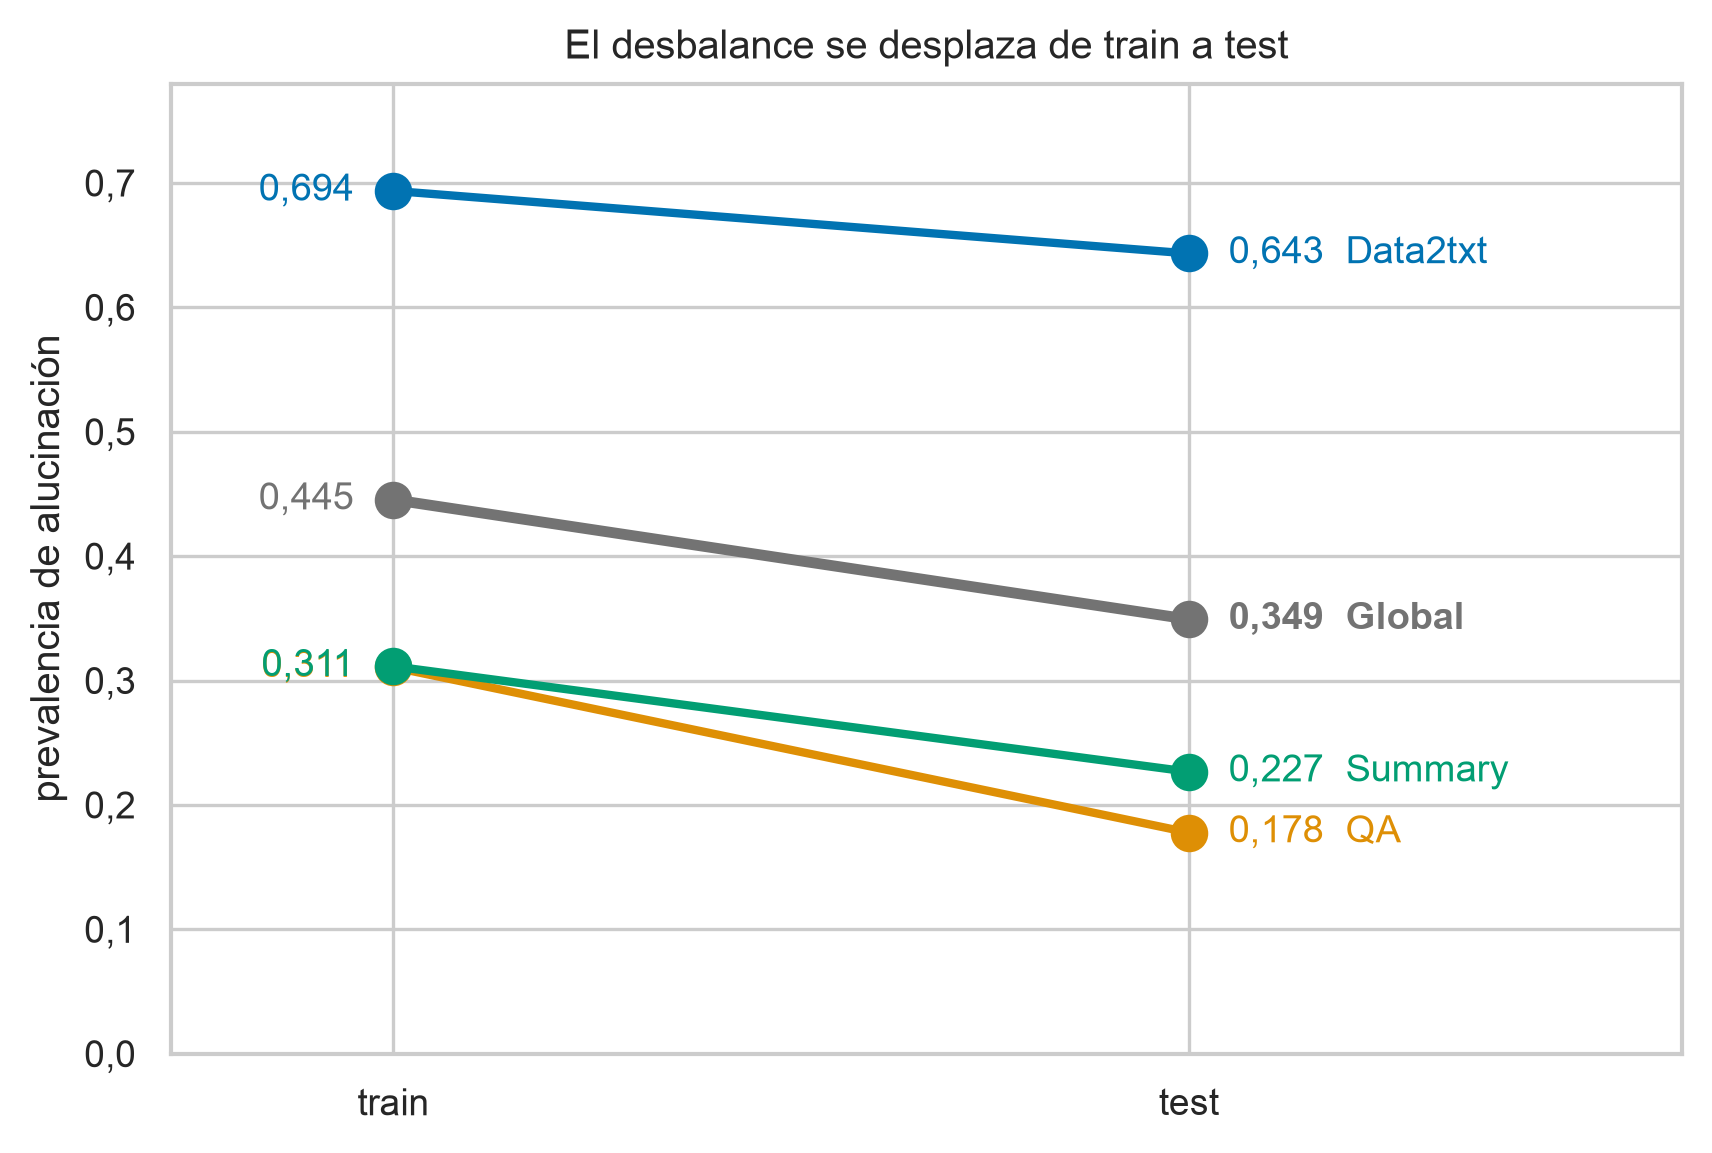
\includegraphics[width=\figw]{desb_prevalencia_tarea}
\caption{Prevalencia por tarea en entrenamiento y test. El desplazamiento del prior es
mayor en QA (0,311 a 0,178), lo que dejará un umbral global demasiado alto para esa tarea.}
\label{fig:prev}
\end{figure}

Estamos ante un desbalance heterogéneo por subgrupo y con desplazamiento de prior. La
consecuencia práctica se anticipa aquí: un único umbral de decisión no puede ser óptimo
para prevalencias tan dispares, y el tratamiento del desbalance no será un ajuste global
sino una decisión por tarea. La distribución de longitudes por clase
(Figura~\ref{fig:eda}) y el reúso de documentos, que motiva el \texttt{GroupKFold},
completan el retrato del conjunto.

\begin{figure}[H]
\centering
\begin{subfigure}{0.48\textwidth}
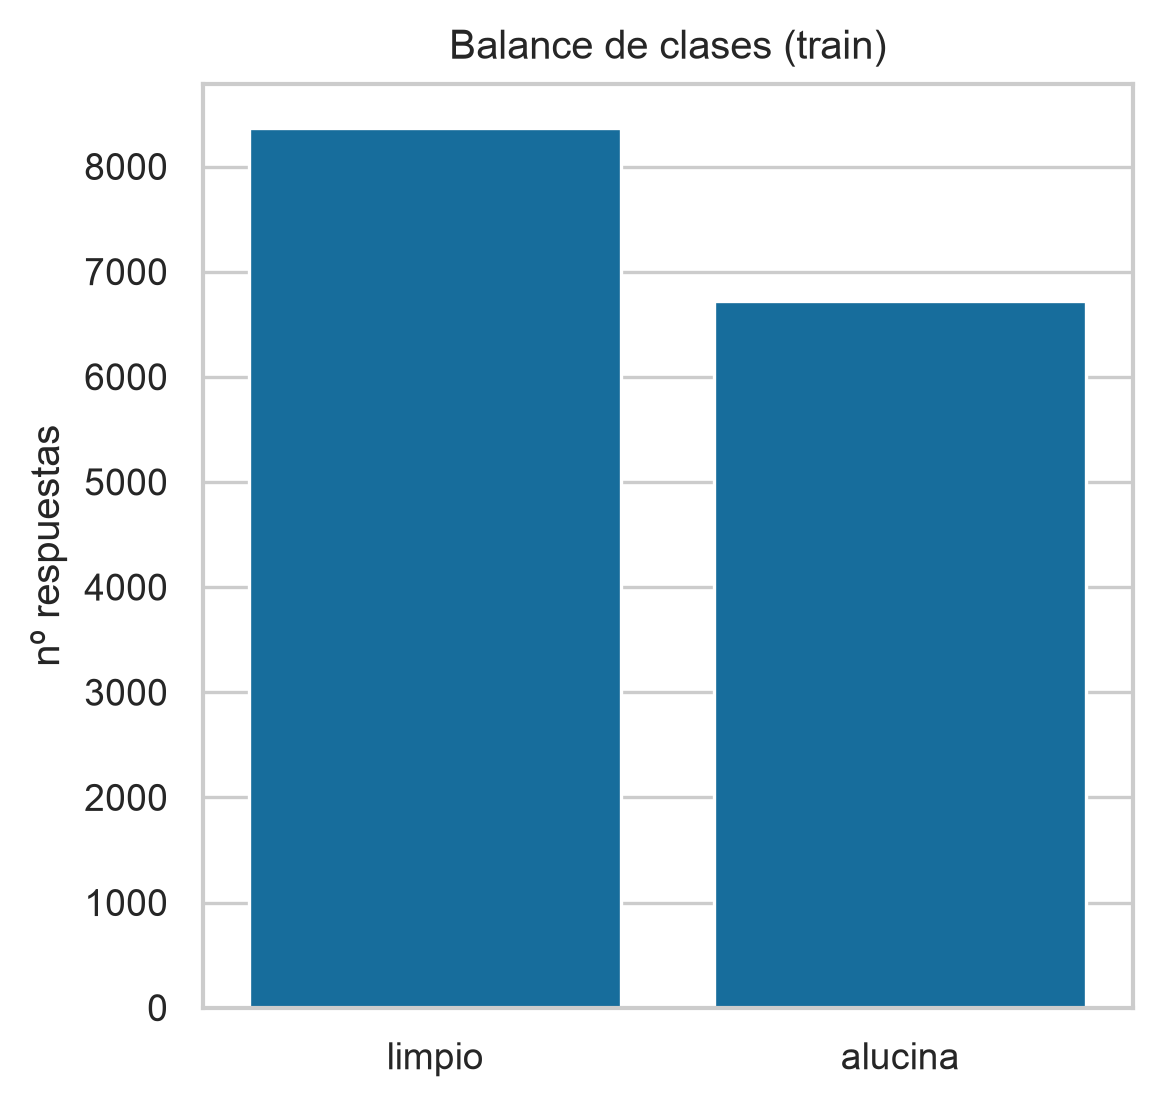
\includegraphics[width=\textwidth]{eda_balance_clases}
\caption{Balance global de clases (train).}
\end{subfigure}\hfill
\begin{subfigure}{0.48\textwidth}
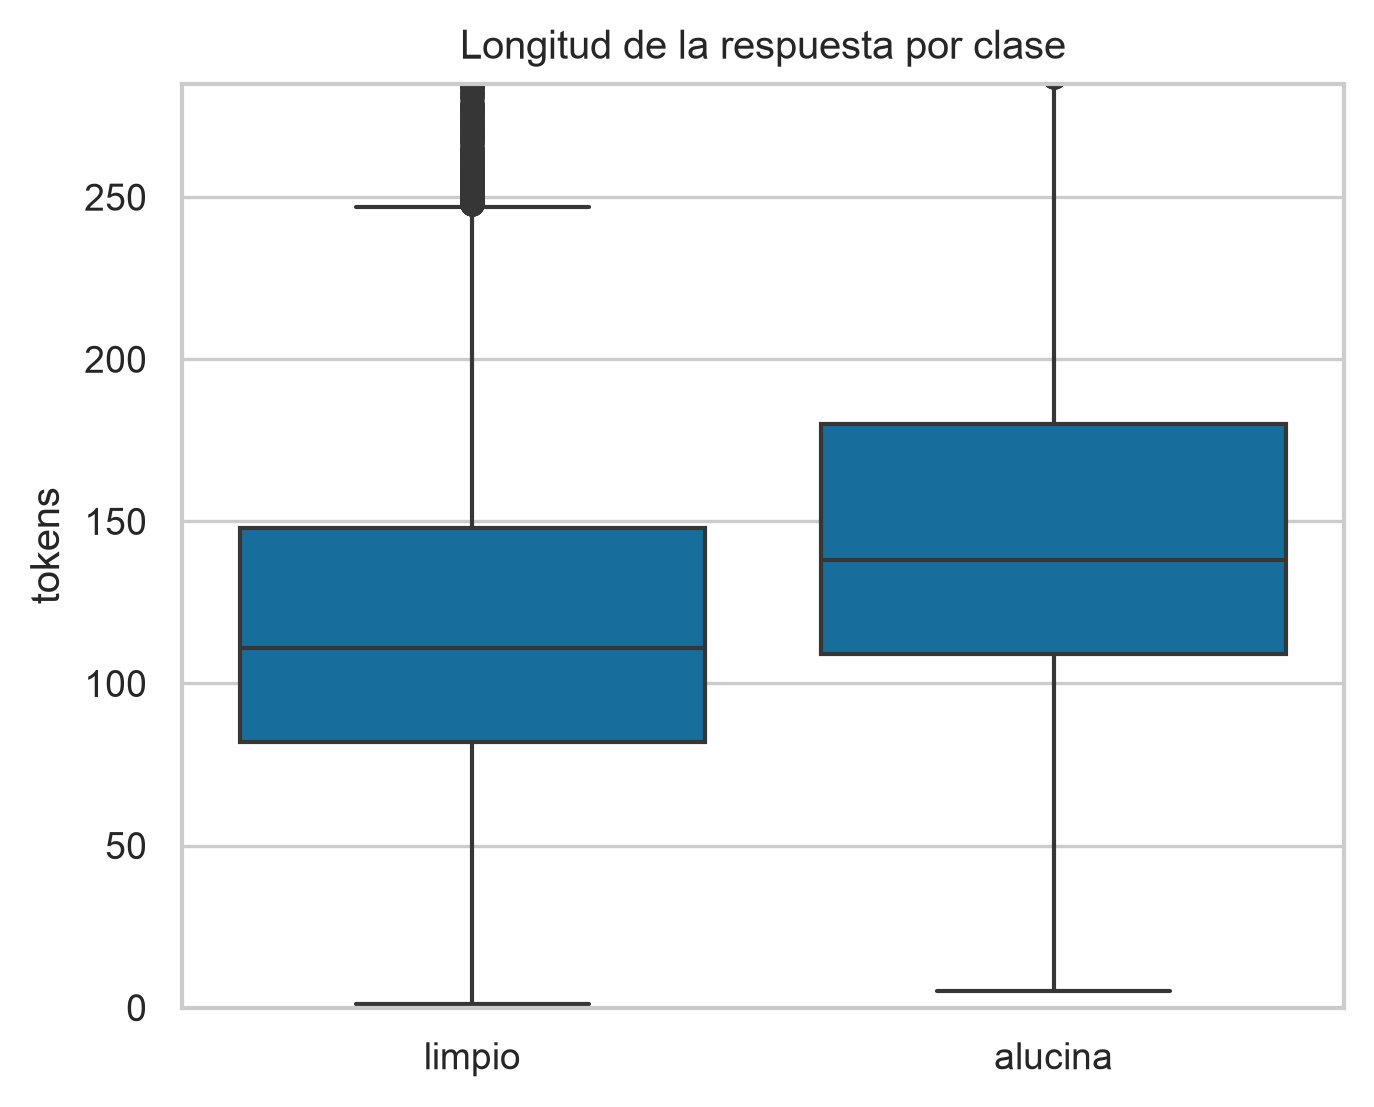
\includegraphics[width=\textwidth]{eda_longitud_por_clase}
\caption{Longitud de la respuesta por clase.}
\end{subfigure}
\caption{Descriptivo global del conjunto de entrenamiento.}
\label{fig:eda}
\end{figure}

\subsection{Caracterización del fenómeno: los tramos alucinados}

Antes de modelar conviene entender qué aspecto tiene una alucinación. Analizamos los
tramos anotados en su posición dentro de la respuesta, su longitud, su categoría
gramatical, el tipo de entidad que contienen y el tipo de alucinación
(Figura~\ref{fig:spans}). Dominan las alucinaciones de números, fechas y nombres
propios, lo que justifica de forma natural las características de solape numérico y de
entidades. La composición por tipo revela un dato que gobierna el capítulo de error:
Summary es en un 86\,\% de tipo evidente, y sin embargo, como veremos, es la tarea más
difícil. El tipo anotado no explica la dificultad.

\begin{figure}[H]
\centering
\begin{subfigure}{0.32\textwidth}
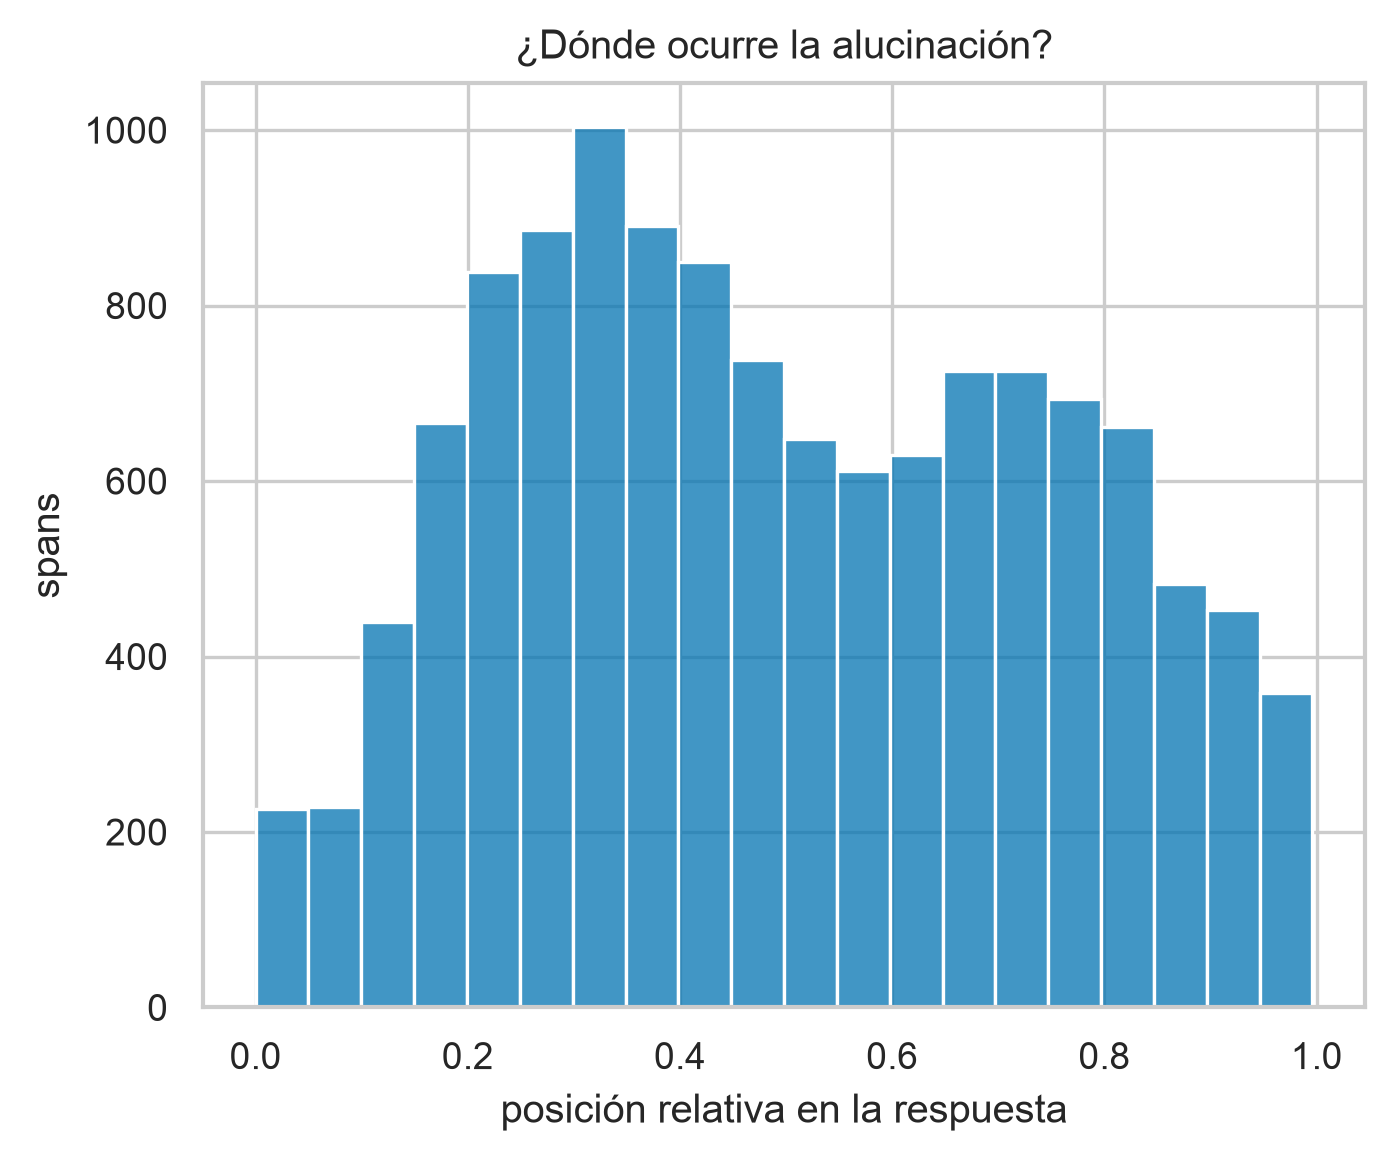
\includegraphics[width=\textwidth]{spans_posicion}
\caption{Posición relativa.}
\end{subfigure}\hfill
\begin{subfigure}{0.32\textwidth}
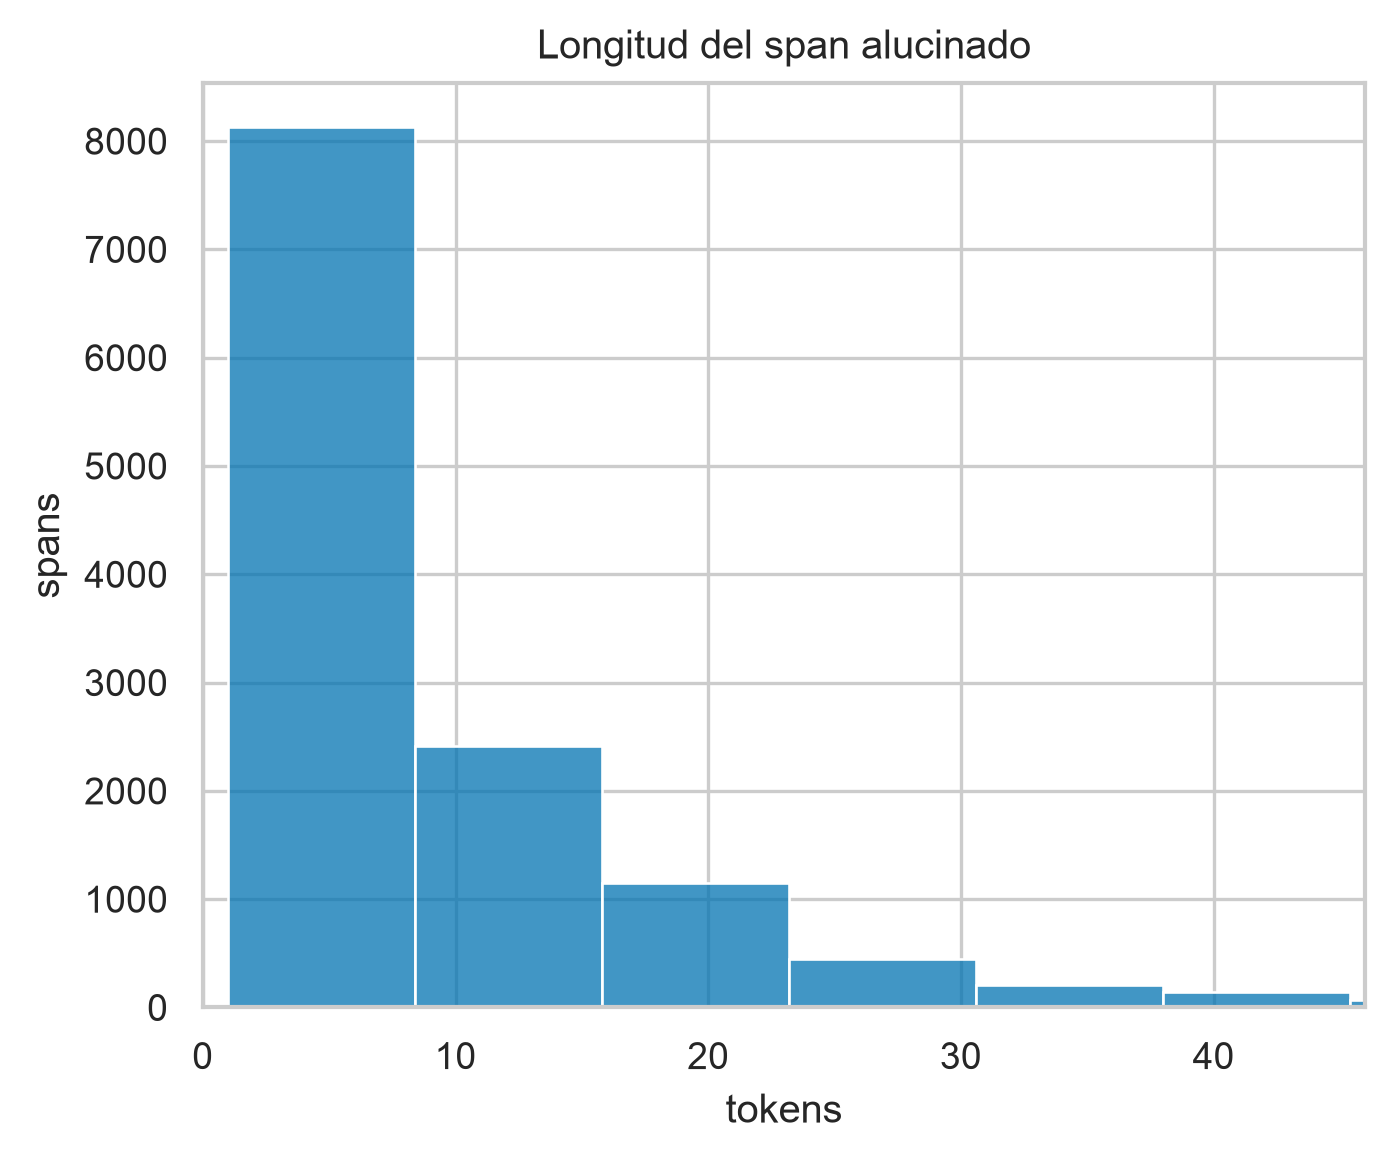
\includegraphics[width=\textwidth]{spans_longitud}
\caption{Longitud (tokens).}
\end{subfigure}\hfill
\begin{subfigure}{0.32\textwidth}
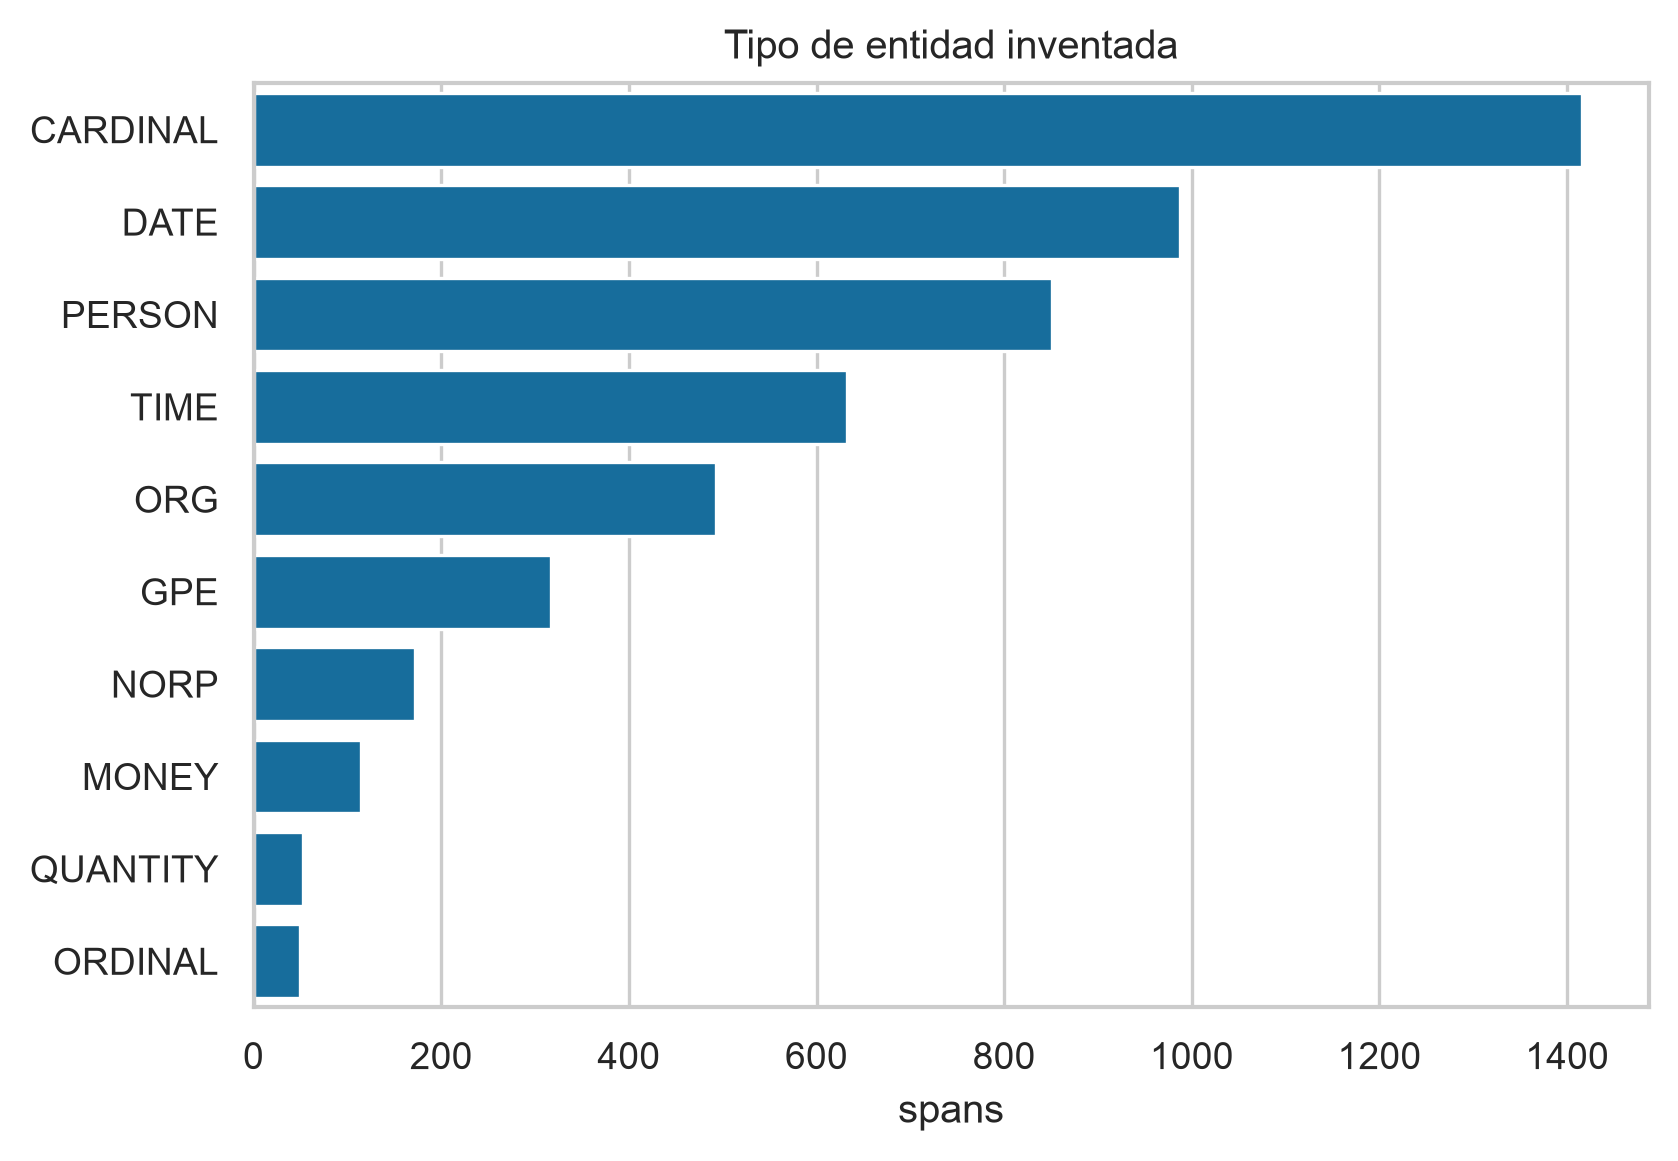
\includegraphics[width=\textwidth]{spans_entidad}
\caption{Tipo de entidad.}
\end{subfigure}

\vspace{0.3cm}
\begin{subfigure}{0.32\textwidth}
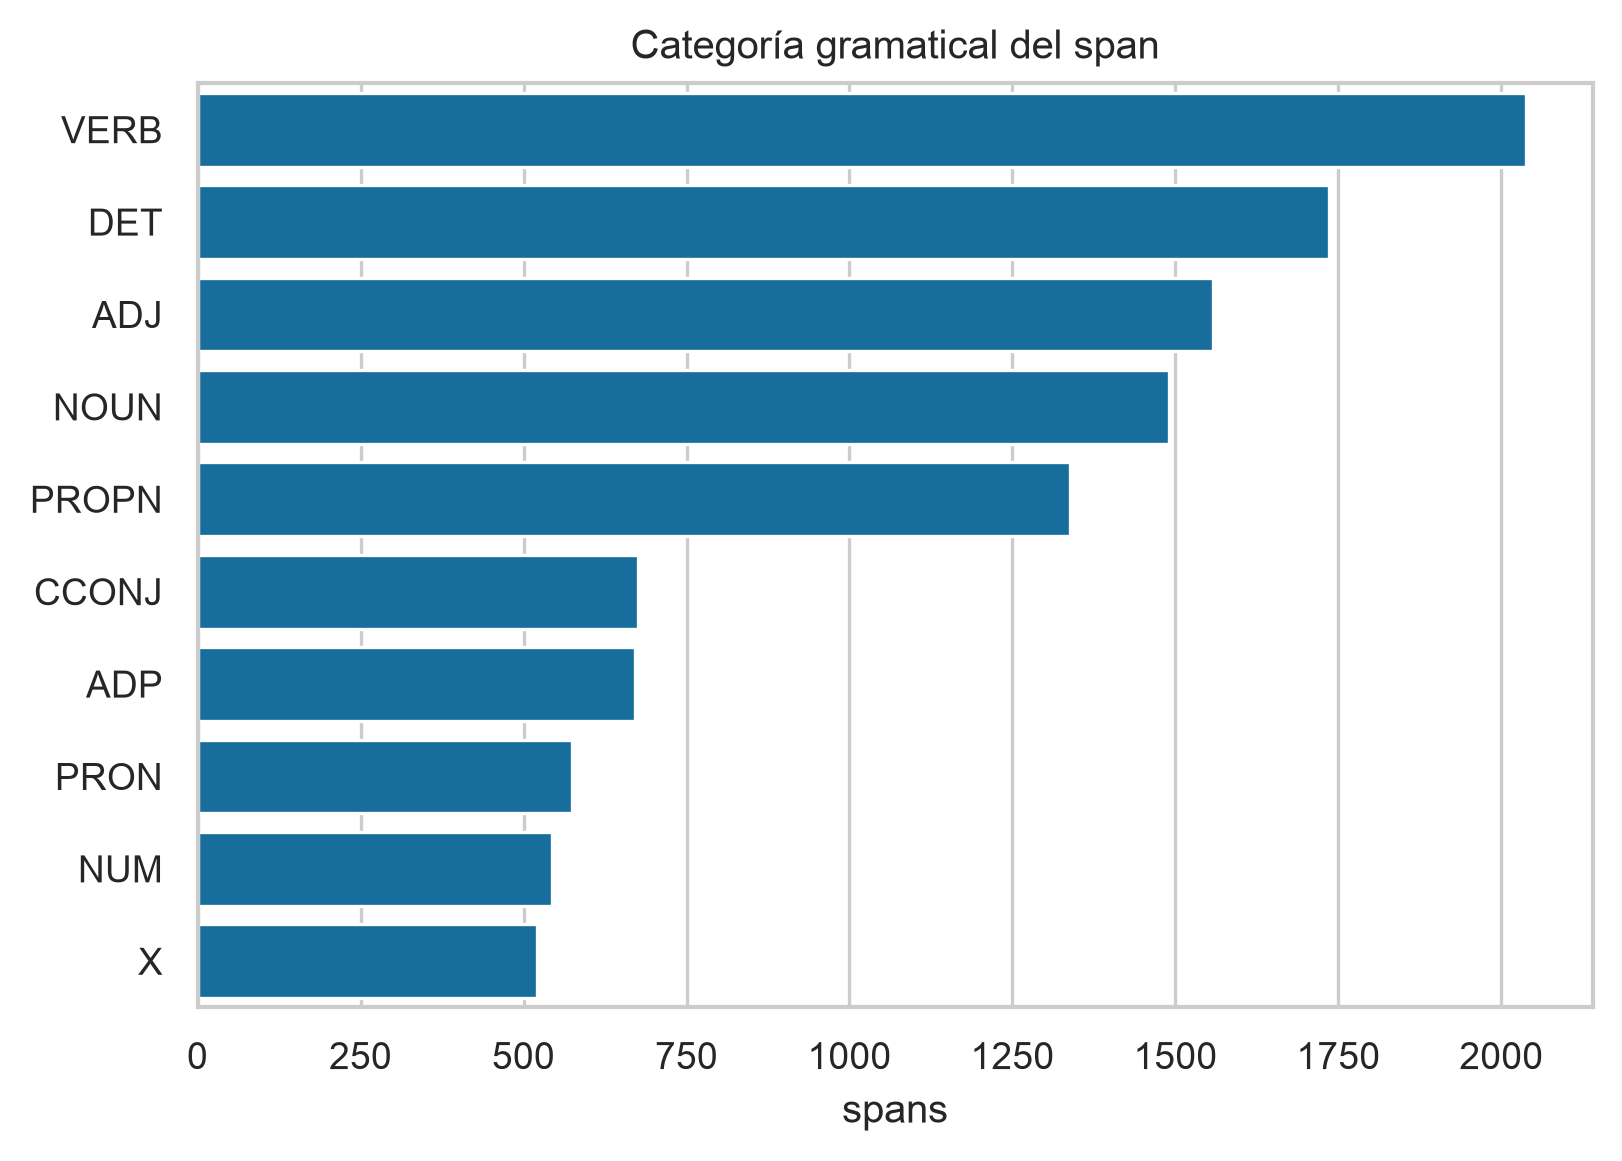
\includegraphics[width=\textwidth]{spans_pos}
\caption{Categoría gramatical.}
\end{subfigure}\hfill
\begin{subfigure}{0.32\textwidth}
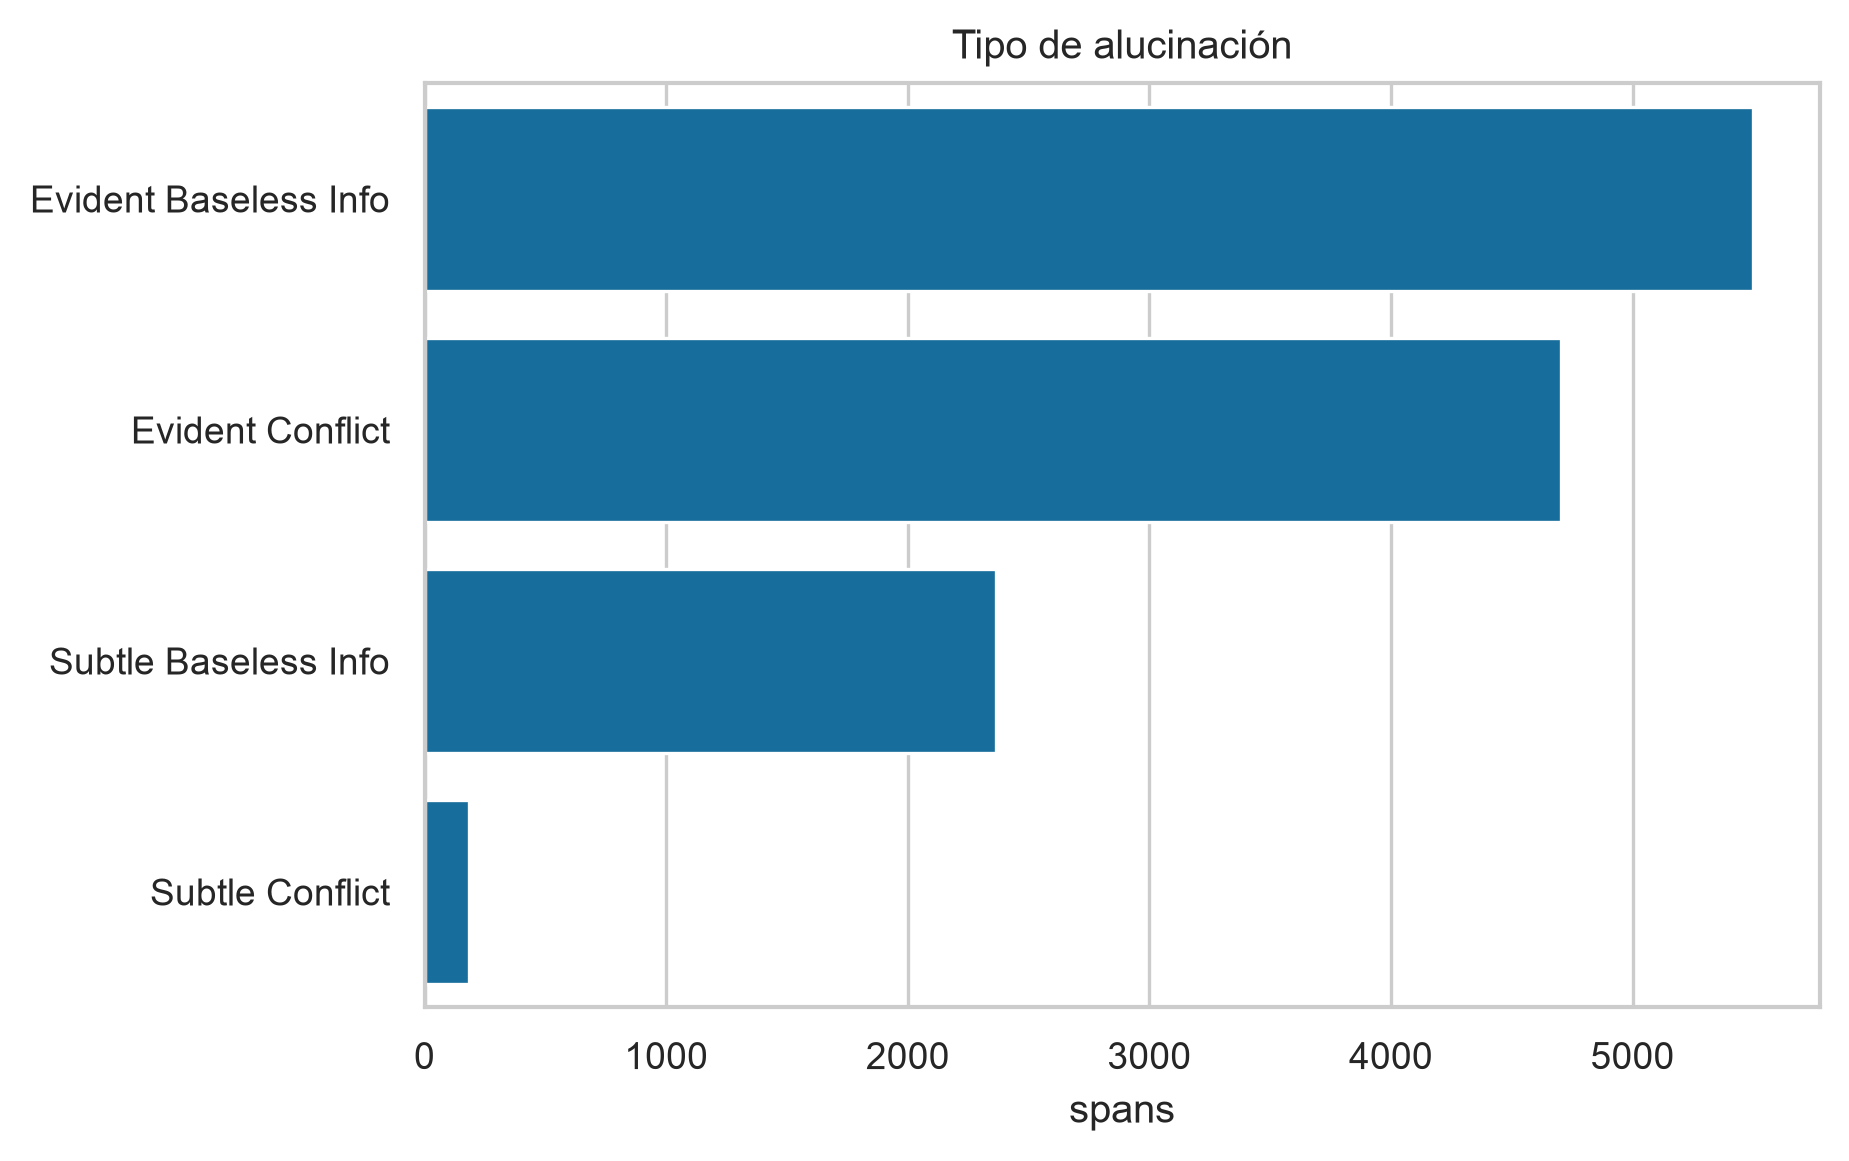
\includegraphics[width=\textwidth]{spans_tipo}
\caption{Tipo de alucinación.}
\end{subfigure}\hfill
\begin{subfigure}{0.32\textwidth}
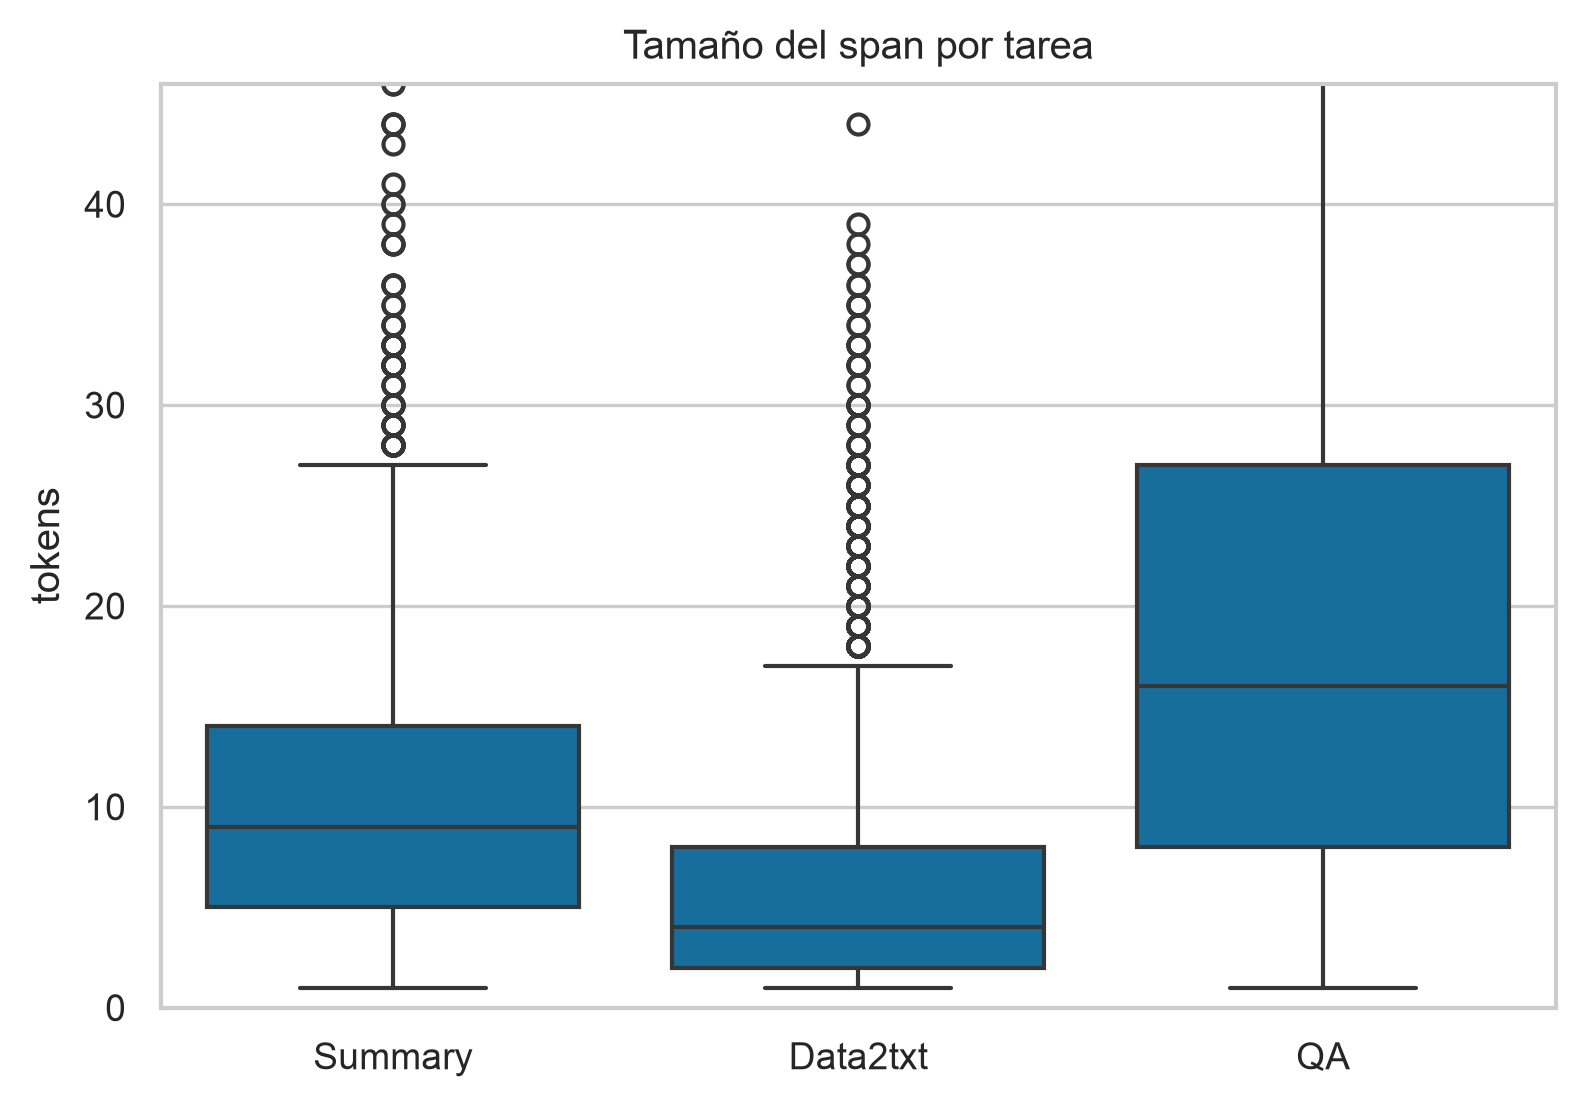
\includegraphics[width=\textwidth]{spans_longitud_por_tarea}
\caption{Longitud por tarea.}
\end{subfigure}
\caption{Descriptivo de los tramos alucinados. Predominan números y entidades; Summary
es mayoritariamente de tipo evidente pese a ser la tarea difícil.}
\label{fig:spans}
\end{figure}

\section{Exploración de características}

\subsection{Catálogo de características}

Construimos la matriz de diseño con tres bloques. El primero son nueve características
escalares sobre el par (respuesta, fuente), que capturan solape léxico, consistencia
numérica y recombinación. El segundo agrega el soporte por frase, con la intuición de
que una alucinación suele ser una frase sin respaldo dentro de una respuesta por lo
demás correcta, y que un promedio sobre toda la respuesta la diluye; por eso agregamos
con el mínimo, que delata la frase peor sostenida. El tercero es la codificación
\emph{one-hot} de la tarea, que permite al modelo especializar su respuesta por tipo de
tarea. El Cuadro~\ref{tab:feats} recoge las dieciocho características.

\begin{table}[H]
\centering
\small
\begin{tabular}{p{3cm}p{10.5cm}}
\toprule
Bloque & Características \\
\midrule
Escalares (9) & \texttt{containment} (precisión léxica $|R\cap F|/|R|$), \texttt{jaccard},
\texttt{tfidf\_cos} (coseno TF-IDF ajustado por par), \texttt{num\_overlap} (números de la
respuesta presentes en la fuente), \texttt{novel\_bigram}, \texttt{novel\_trigram}
(recombinación de $n$-gramas), \texttt{num\_context} (consistencia número-unidad),
\texttt{neg\_diff} (diferencia de negación), \texttt{answer\_len} \\
\midrule
Nivel frase (6) & \texttt{sent\_cont\_min}, \texttt{sent\_cont\_mean}, \texttt{sent\_cont\_std},
\texttt{sent\_frac\_low}, \texttt{sent\_sim\_min}, \texttt{sent\_sim\_mean} \\
\midrule
One-hot tarea (3) & \texttt{task\_QA}, \texttt{task\_Summary}, \texttt{task\_Data2txt} \\
\bottomrule
\end{tabular}
\caption{Las dieciocho características. $R$ y $F$ son los conjuntos de palabras únicas de
respuesta y fuente. El coseno TF-IDF sigue el modelo de espacio vectorial
\cite{salton1988tfidf}.}
\label{tab:feats}
\end{table}

La característica \texttt{containment}, la fracción de palabras de la respuesta que
aparecen en la fuente, es la señal dominante, y su signo es el esperado: más solape
léxico implica menos probabilidad de alucinación. La codificación de tarea y el coseno
TF-IDF se mantienen en el modelo por su papel funcional, la primera para especializar
por tarea y la segunda como medida semántica clásica, aunque su aporte marginal sea
pequeño una vez presente \texttt{containment}, como cuantificamos más abajo. La
separabilidad univariada de cada característica por clase aparece en la
Figura~\ref{fig:sep}.

\begin{figure}[H]
\centering
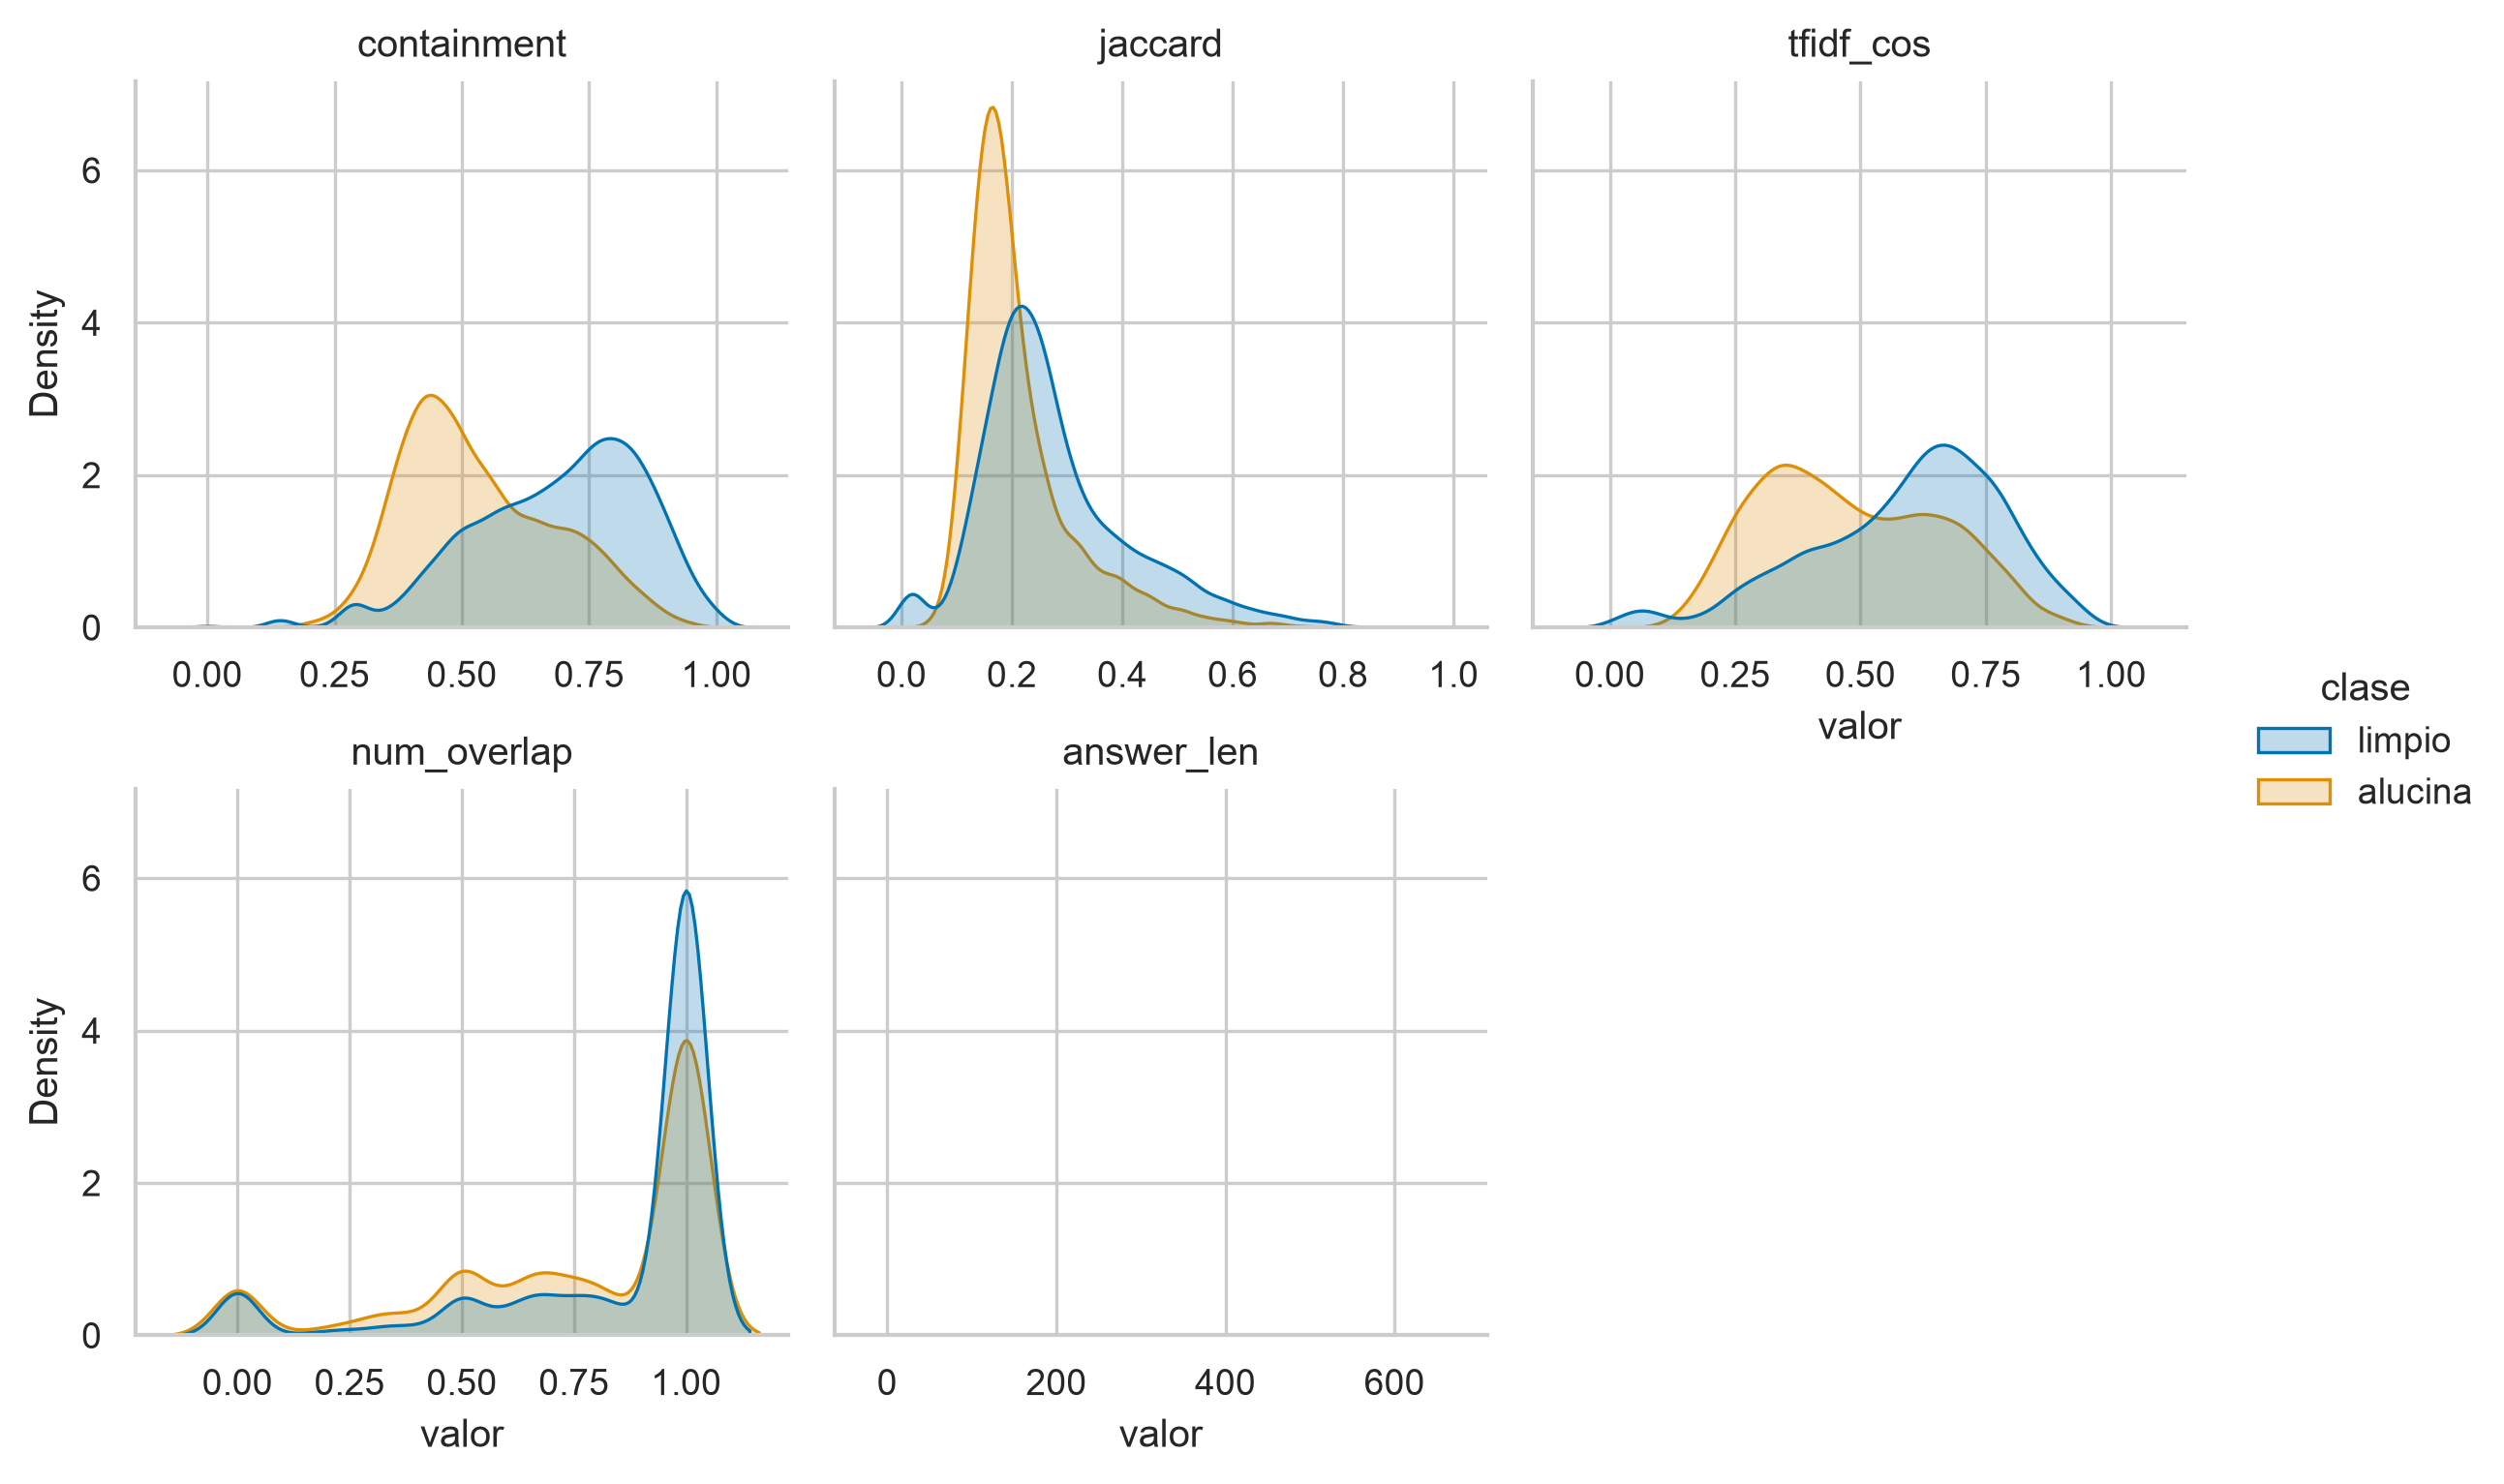
\includegraphics[width=\figw]{eda_separabilidad_features}
\caption{Distribución de cada característica separada por clase. \texttt{containment} y
las medidas de solape muestran el mayor desplazamiento entre limpio y alucinado.}
\label{fig:sep}
\end{figure}

\subsection{Características probadas y descartadas}

La exploración de características incluye varias vías que no funcionaron. Las
documentamos porque forman parte de la caracterización del techo del problema: no es que
no se intentara. El Cuadro~\ref{tab:descartadas} recoge cada vía y la cifra que la
descartó, siempre medida con el protocolo honesto.

\begin{table}[H]
\centering
\small
\begin{tabular}{p{3.2cm}p{6.3cm}p{3.8cm}}
\toprule
Vía & Qué es & Resultado \\
\midrule
LSA & TF-IDF con descomposición en valores singulares truncada
\cite{deerwester1990lsa,halko2011svd}, ajustada por partición & $+0,001$ de AUC global;
redundante con \texttt{containment} \\
\texttt{sent\_novel} & Novedad de $n$-gramas agregada por frase & $+0,001$ global; el
resumen fiel recombina igual que el alucinado \\
Estructura sintáctica & Arcos de dependencia, sujeto-verbo-objeto y enlace
entidad-número con spaCy & Summary $0{,}701 \to 0{,}700$ \\
\bottomrule
\end{tabular}
\caption{Vías de características exploradas y descartadas. Cuatro familias distintas,
solape léxico, similitud por frase, recombinación de $n$-gramas y estructura sintáctica,
fracasan por el mismo motivo en Summary: resumir es recombinar, y el texto fiel comparte
la firma de superficie con el alucinado.}
\label{tab:descartadas}
\end{table}

\subsection{Redundancia y selección de variables}

Con dieciocho características cabe preguntarse si sobran. Tres análisis convergen en que
sí hay redundancia, pero no sobreajuste peligroso. La correlación de Spearman
(Figura~\ref{fig:featcorr}) muestra que el bloque de solape está muy correlacionado,
con pares como \texttt{novel\_bigram} y \texttt{novel\_trigram} en 0,98; hay del orden de
dos o tres señales independientes en trece características. Una selección hacia delante
por modelo aplana la curva de F1 pronto, con una rodilla alrededor de ocho
características (Figura~\ref{fig:fsel}). Y al comparar el modelo podado con el completo
en el test oficial, pasar de siete a dieciocho características aporta 0,006 de AUC y
0,004 de F1, dentro del ruido.

\begin{figure}[H]
\centering
\begin{subfigure}{0.48\textwidth}
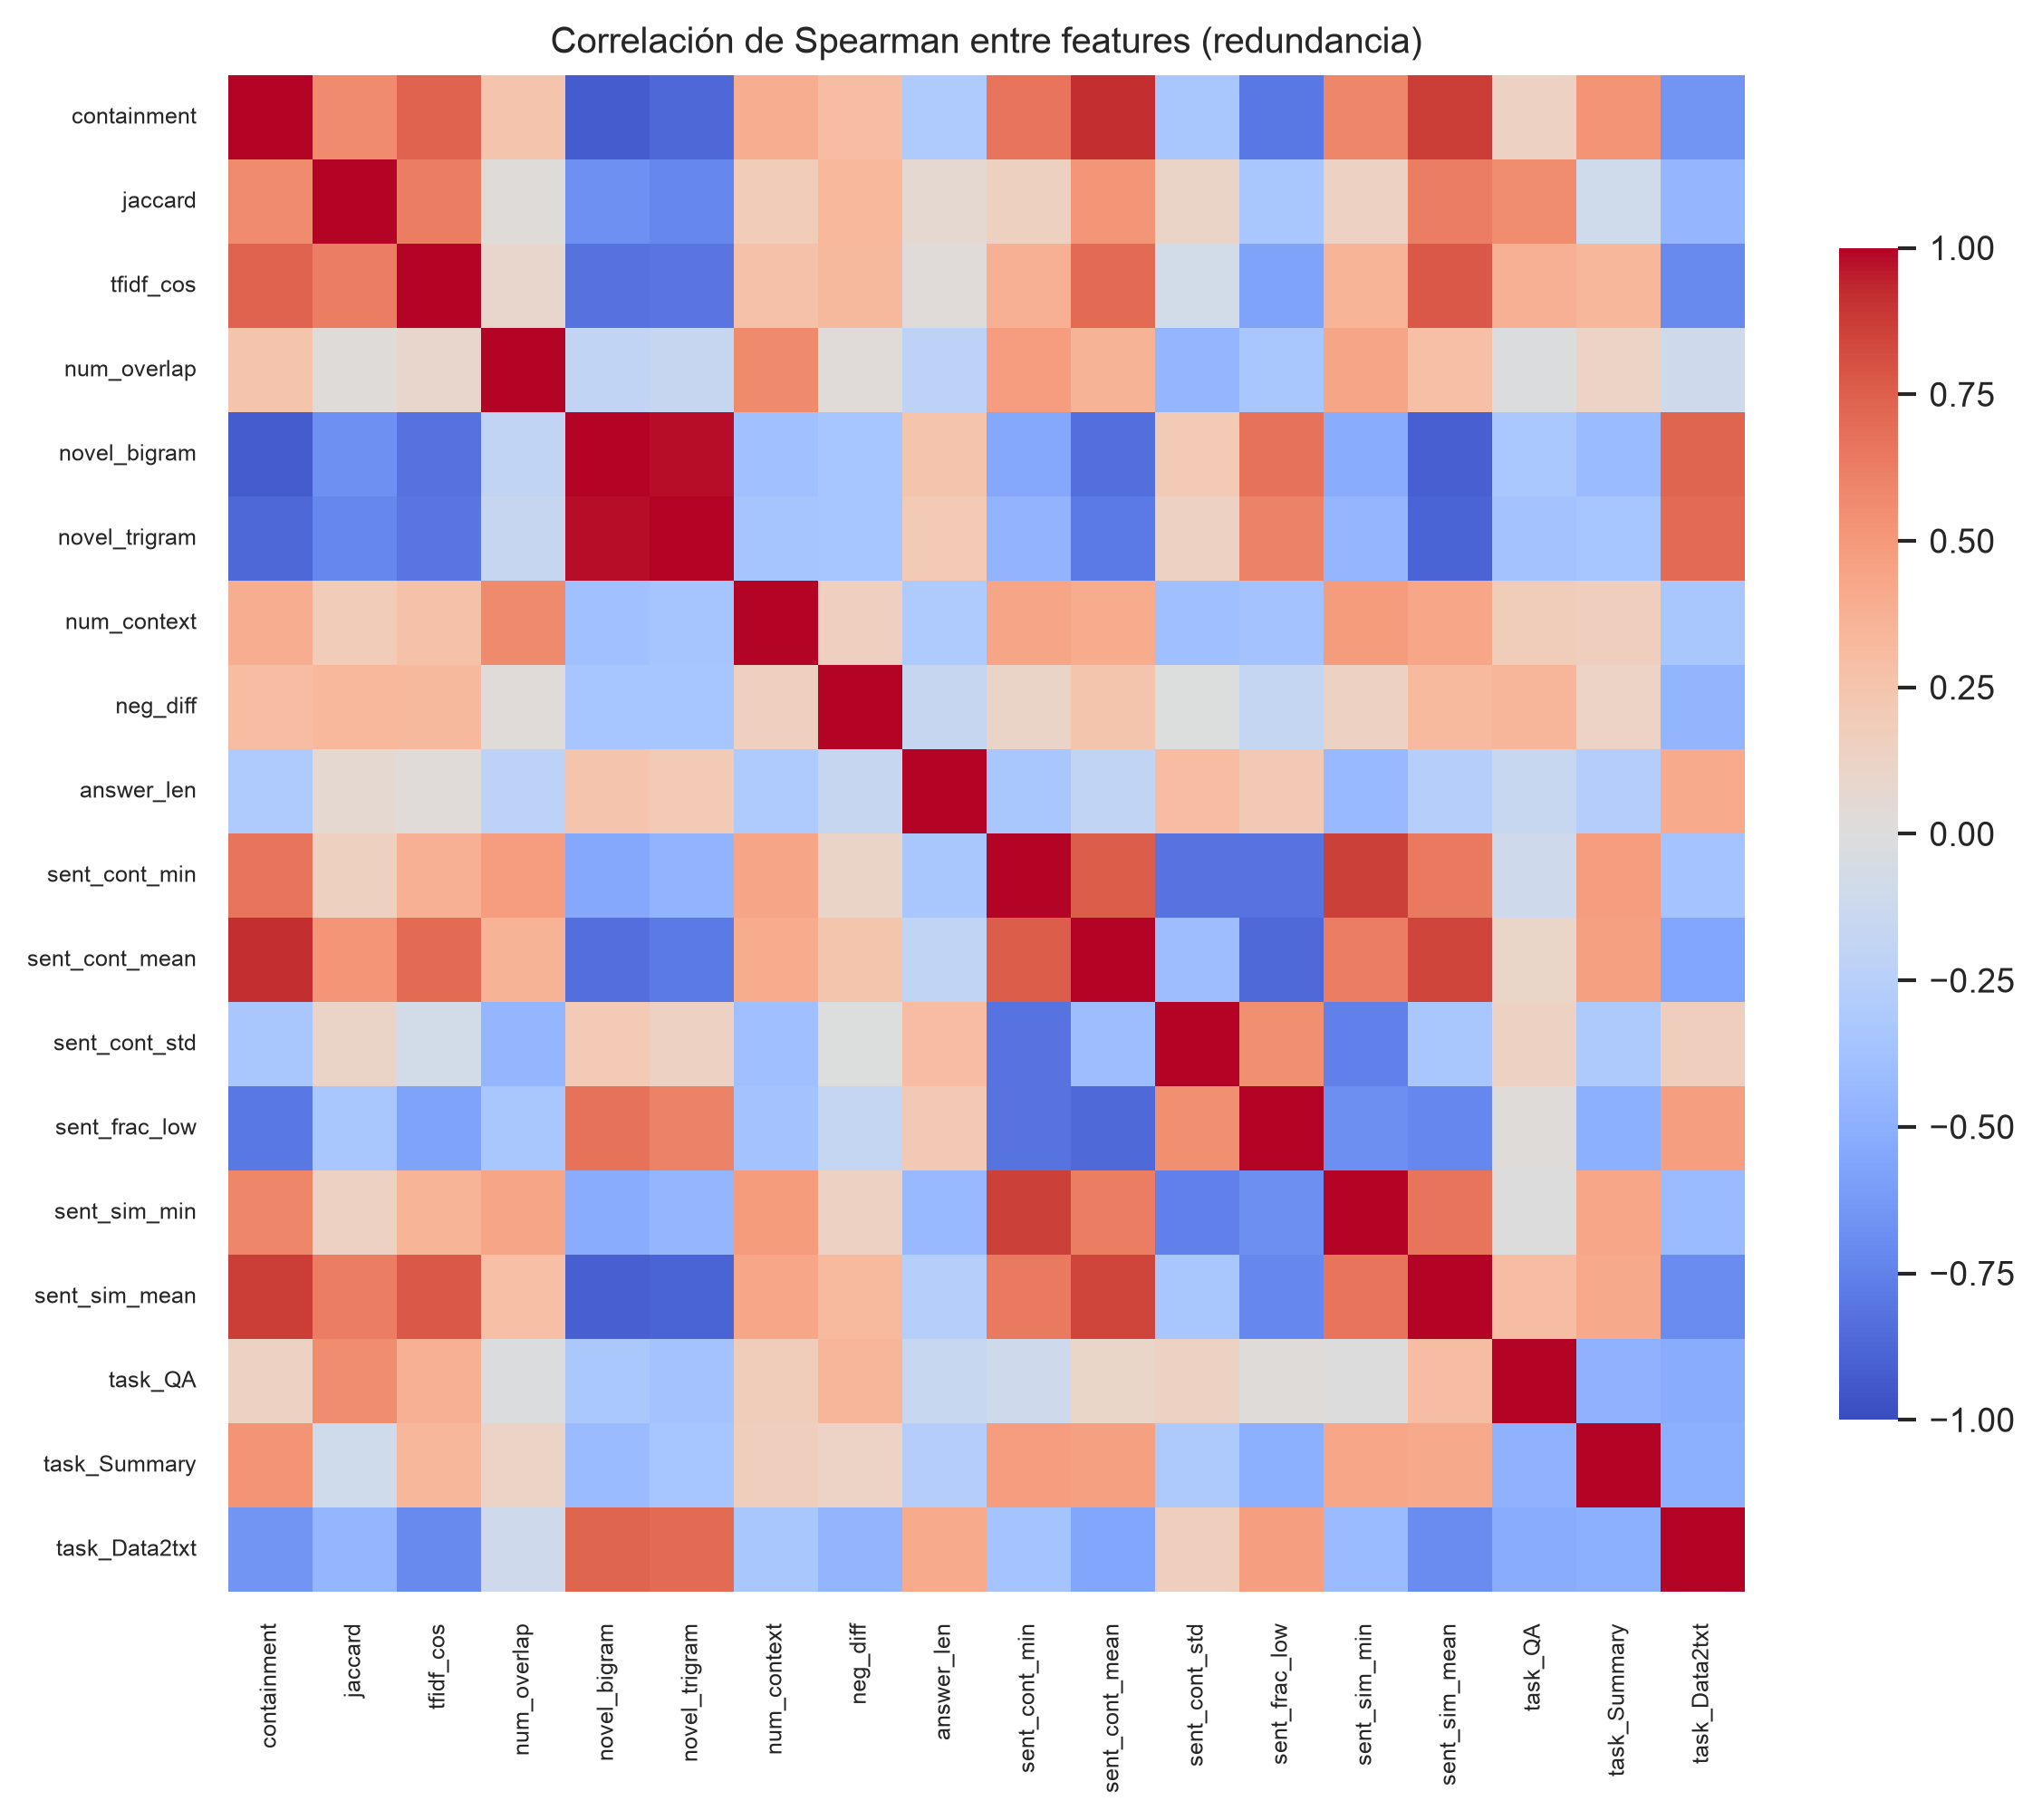
\includegraphics[width=\textwidth]{feat_correlacion}
\caption{Correlación de Spearman entre características.}
\label{fig:featcorr}
\end{subfigure}\hfill
\begin{subfigure}{0.48\textwidth}
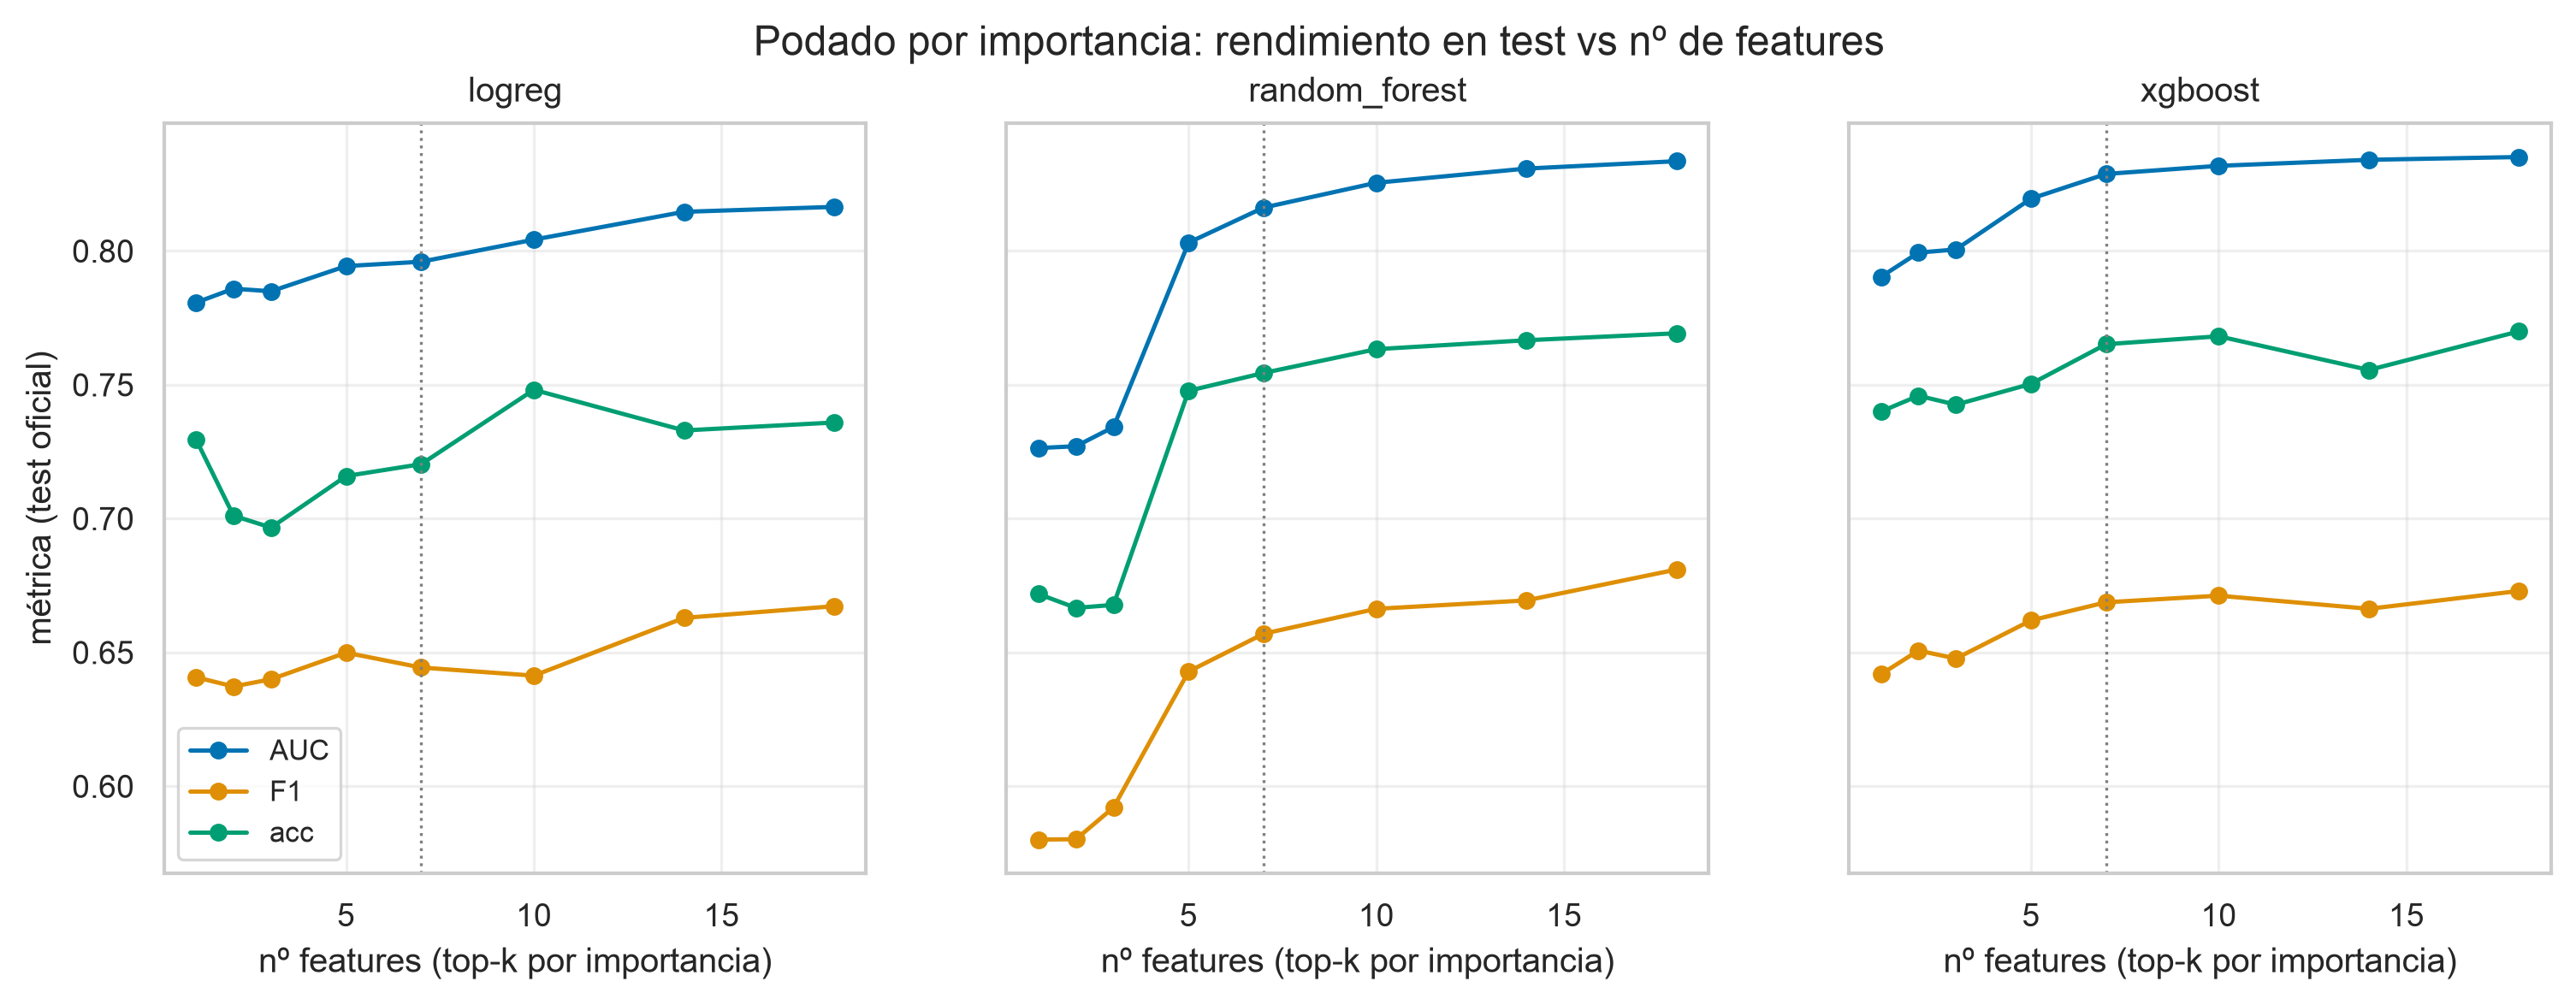
\includegraphics[width=\textwidth]{feat_podado_test}
\caption{Rendimiento frente a número de características (test).}
\end{subfigure}
\caption{Redundancia y parsimonia. Siete características igualan a las dieciocho.}
\end{figure}

\begin{figure}[H]
\centering
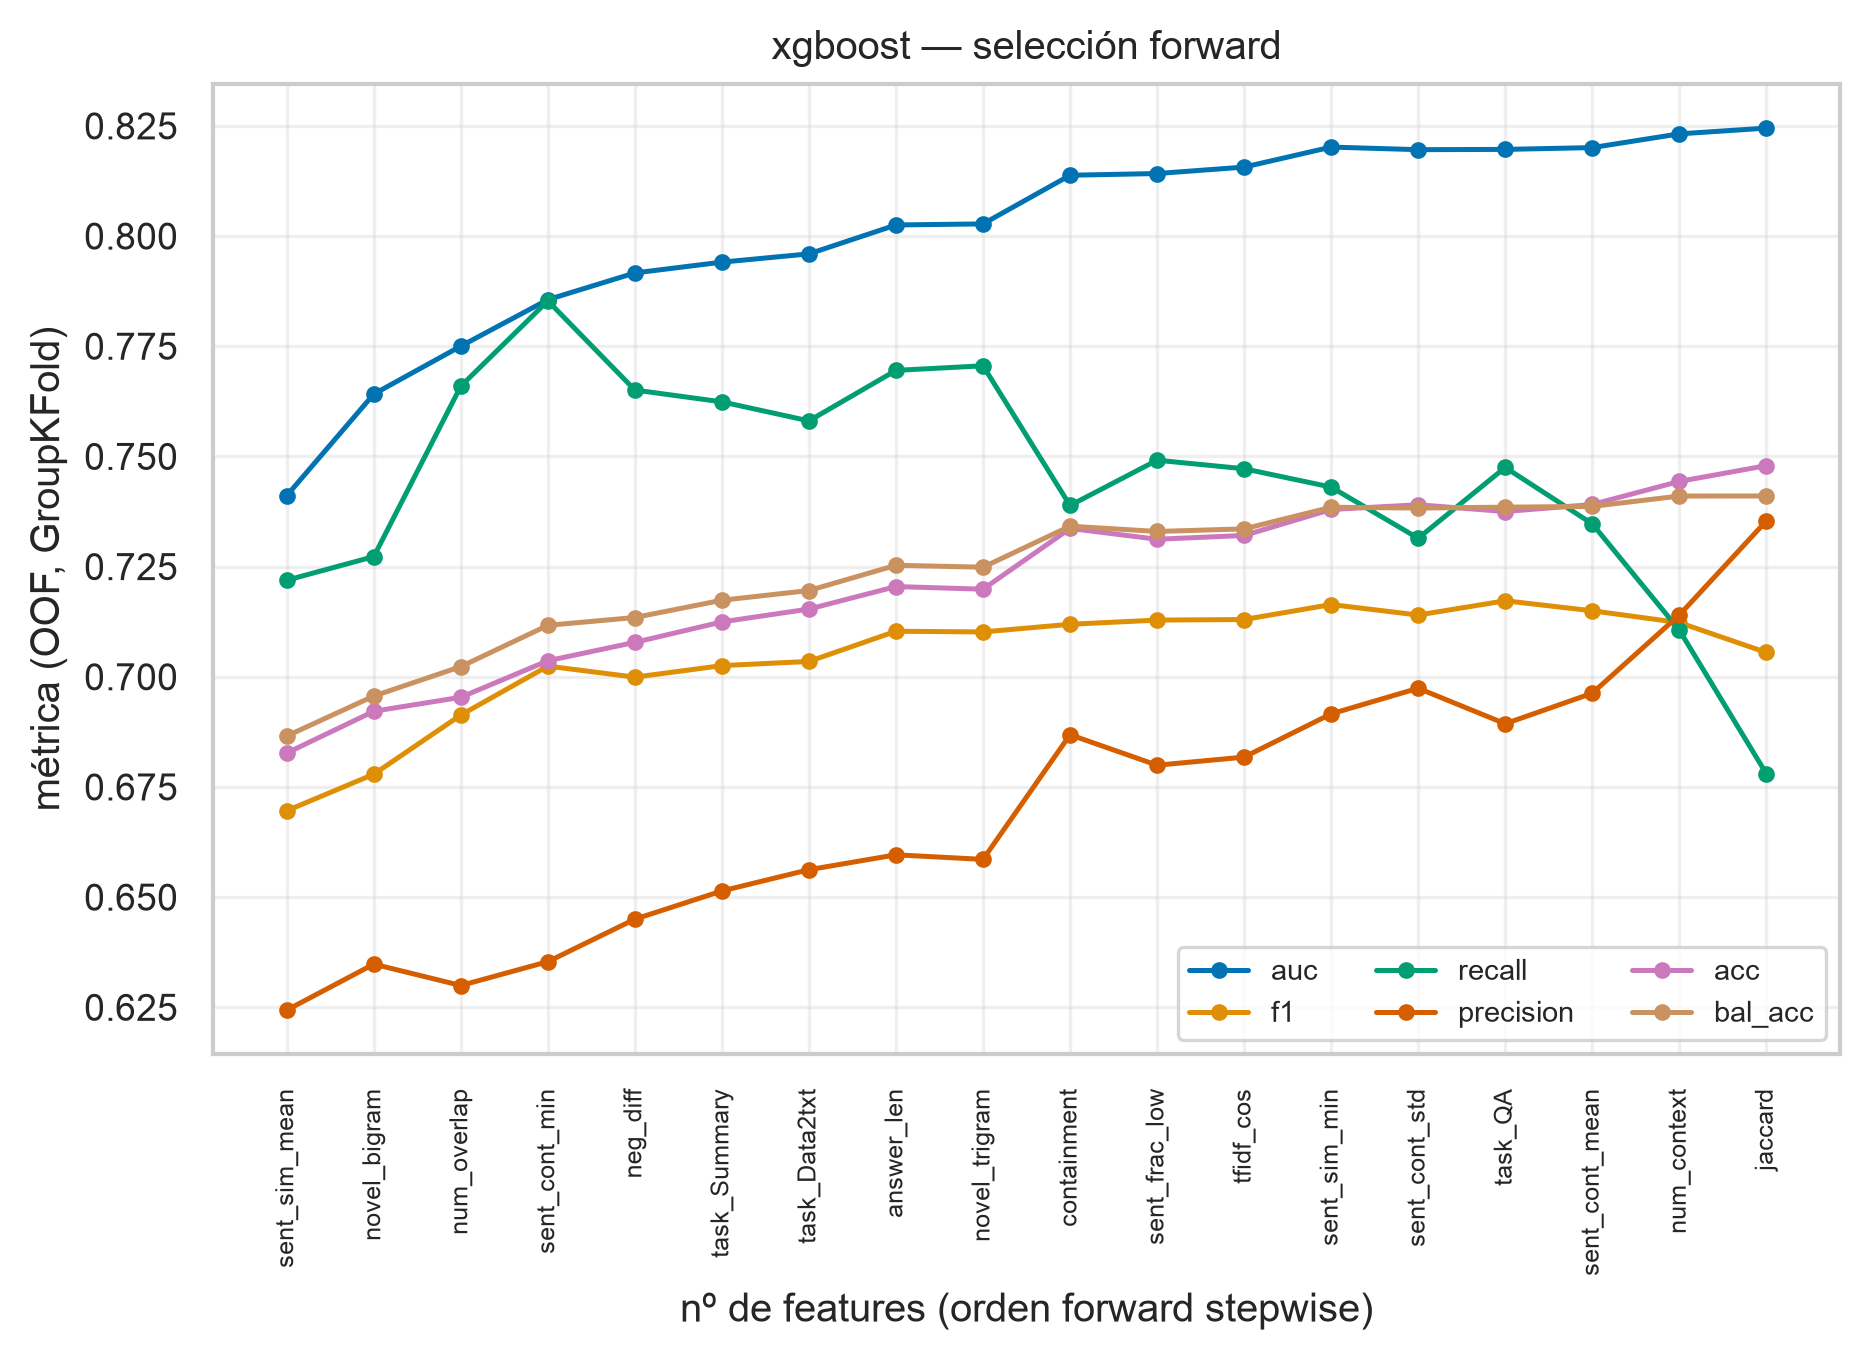
\includegraphics[width=\figw]{fsel_xgboost}
\caption{Selección hacia delante (XGBoost). Cada métrica frente a la incorporación
ordenada de características. La curva se satura pronto: \texttt{containment} carga con
casi toda la señal.}
\label{fig:fsel}
\end{figure}

\subsection{Qué características explican el rendimiento}

La importancia por permutación mide cuánto cae el AUC real al romper cada característica.
El resultado es contundente: \texttt{containment} explica unas ocho veces más que la
siguiente (Figura~\ref{fig:imp}). Rompiéndola, el AUC cae dieciséis puntos; rompiendo
cualquier otra, menos de dos. La importancia acumulada cruza el 80\,\% con muy pocas
características. Al desglosar por tarea aparece un matiz valioso: en Data2txt la
característica relacional \texttt{num\_context} es la primera, por encima de
\texttt{containment}, porque la consistencia número-unidad es lo que caza las cifras
fabricadas; en QA y Summary casi todo depende del solape léxico.

\begin{figure}[H]
\centering
\begin{subfigure}{0.48\textwidth}
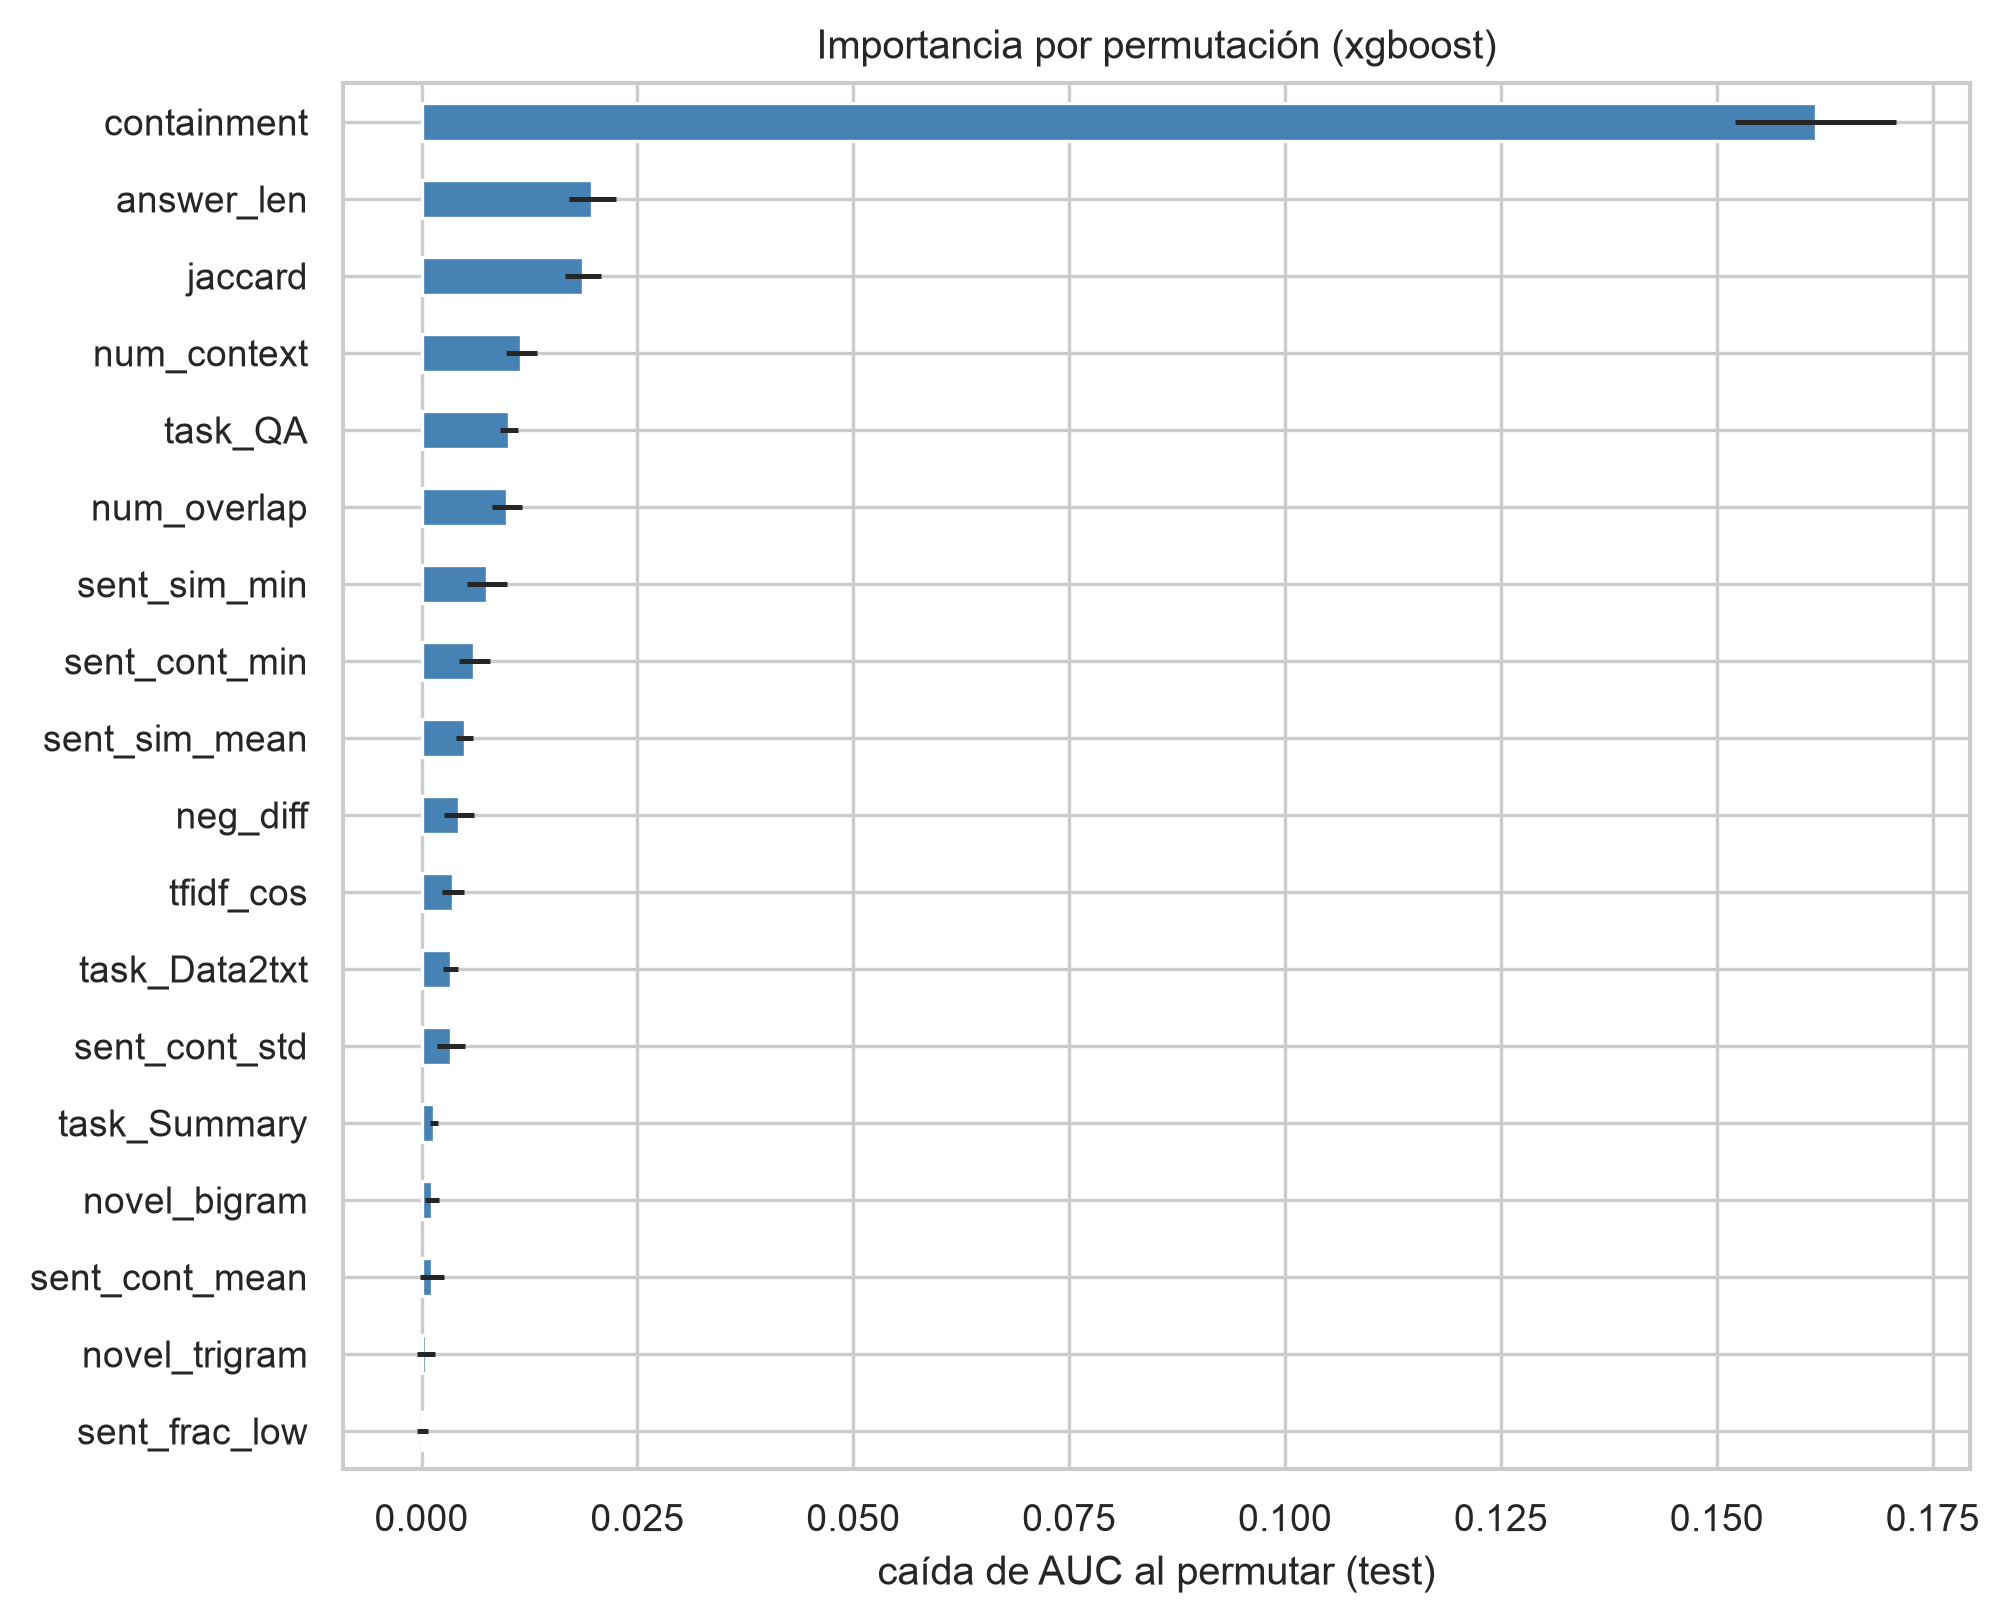
\includegraphics[width=\textwidth]{feat_importancia_perm}
\caption{Importancia por permutación (caída de AUC).}
\end{subfigure}\hfill
\begin{subfigure}{0.48\textwidth}
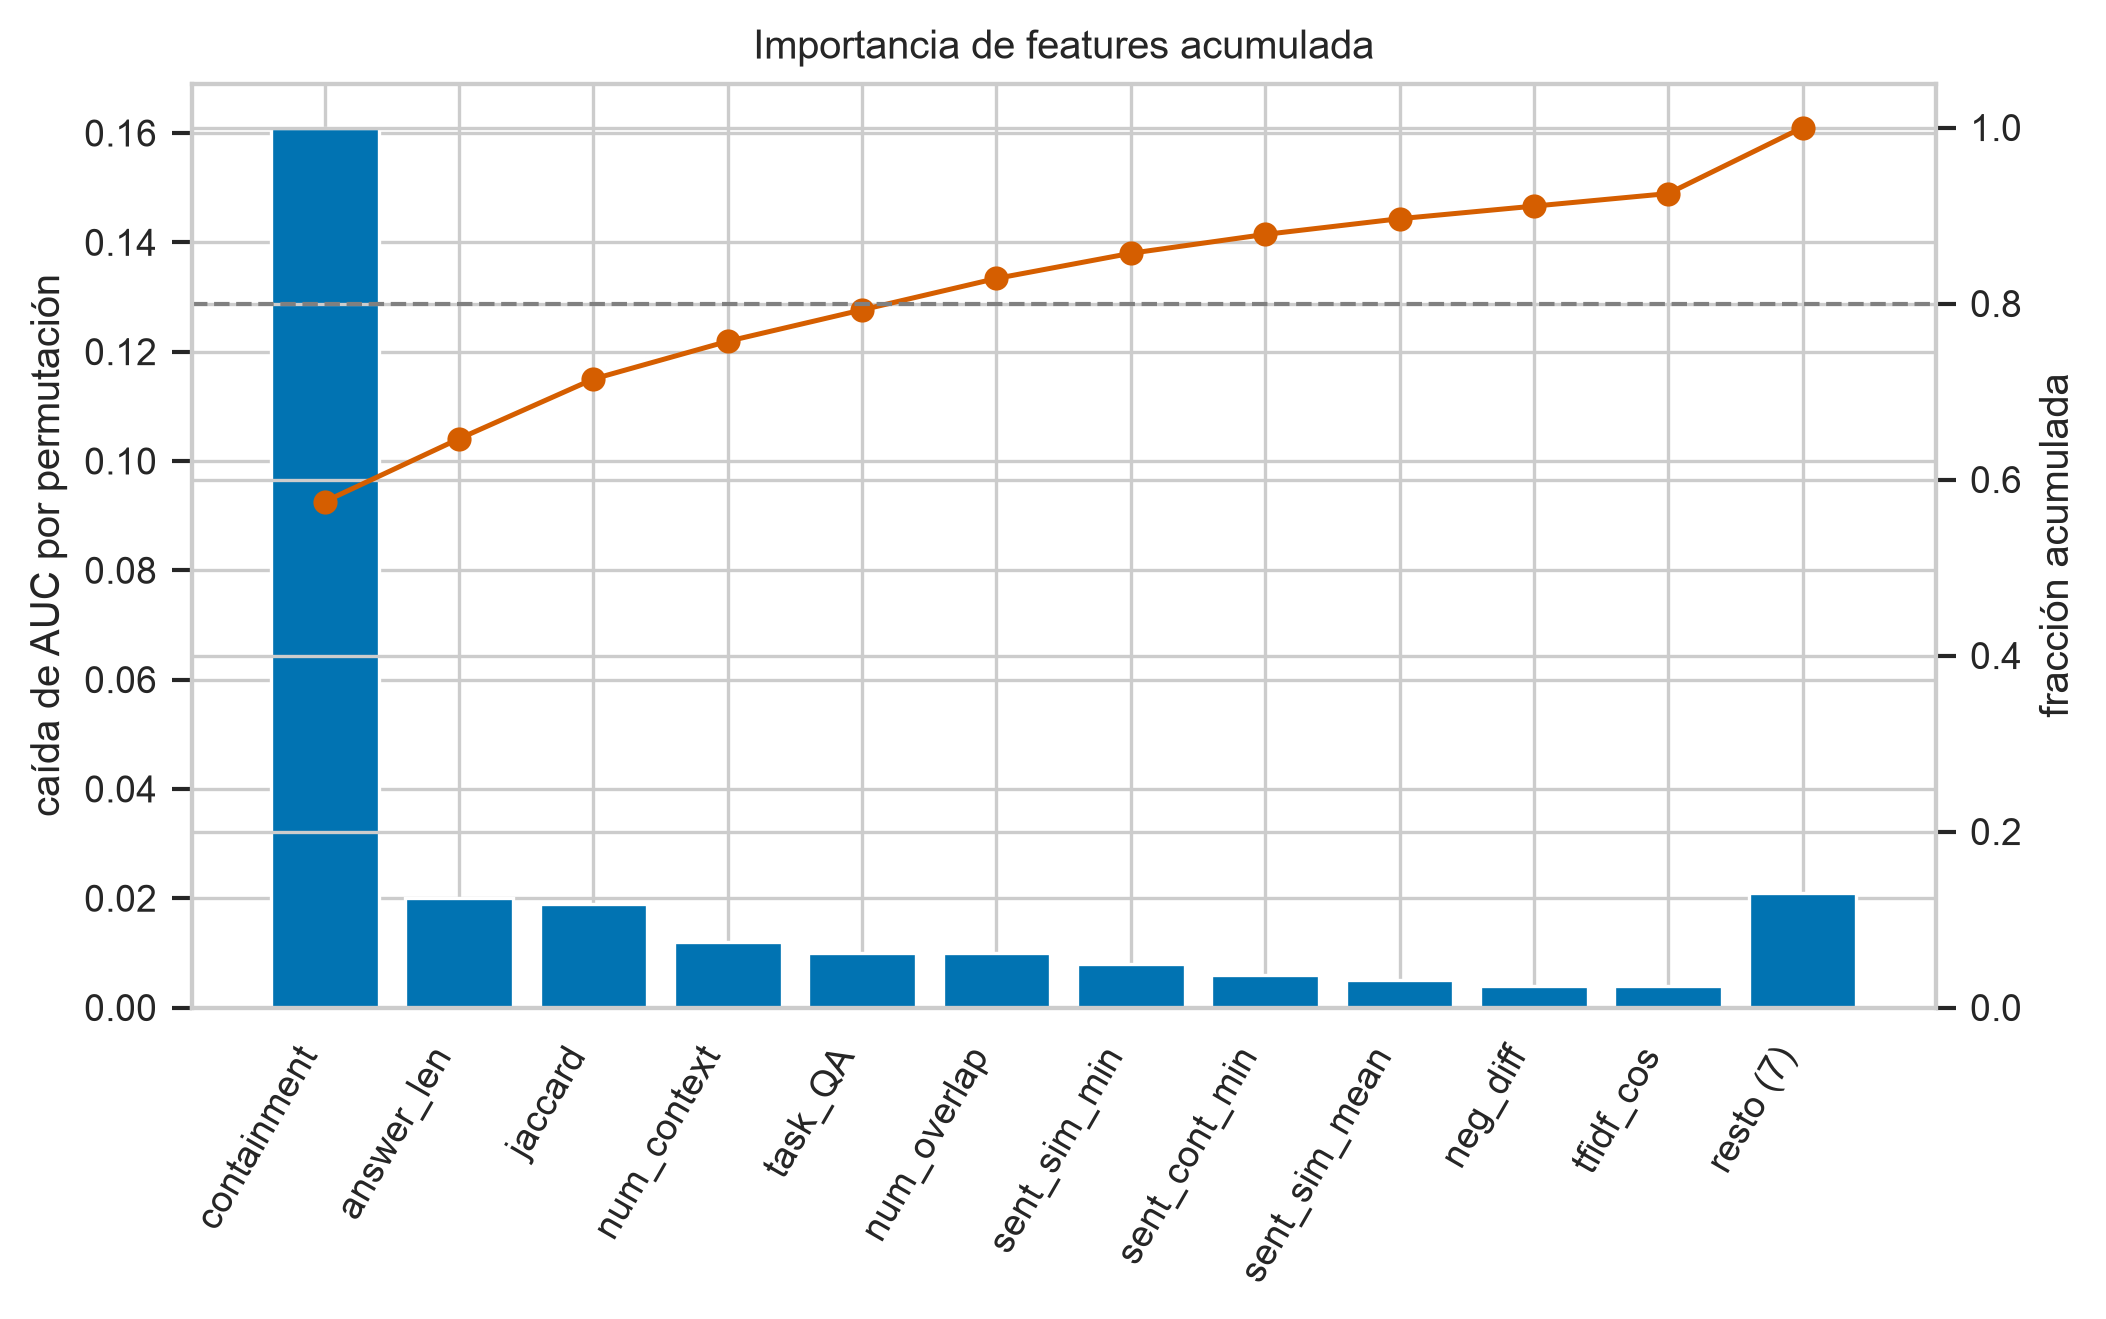
\includegraphics[width=\textwidth]{feat_importancia_acumulada}
\caption{Importancia acumulada.}
\end{subfigure}
\caption{Una única característica léxica trivial carga con casi toda la señal, lo que da
al detector su carácter interpretable.}
\label{fig:imp}
\end{figure}

\paragraph{Decisión.} Mantenemos el conjunto completo de dieciocho características como
base del detector, con la codificación de tarea y el coseno TF-IDF incluidos por su papel
funcional. La redundancia está caracterizada y, si se busca parsimonia, siete
características reproducen el rendimiento; conservamos las demás porque en el test no
penalizan y aportan interpretabilidad por tarea.

\section{Tratamiento del desbalance de clases}

\subsection{Diagnóstico: dos poblaciones de falsos negativos}

El detector deja pasar demasiadas alucinaciones, y esta es la preocupación central del
capítulo. Antes de tratar el desbalance, distinguimos dos causas de falso negativo que
exigen remedios distintos. El análisis de error por tarea (Figura~\ref{fig:err}) lo
separa con claridad.

La primera población vive en QA. Su AUC es 0,822, el mejor de las tres tareas, de modo
que el modelo ordena las alucinaciones casi a la perfección; sin embargo, con un umbral
global solo recupera el 54\,\% de ellas. Esto no es un problema de señal, sino de
decisión: el umbral, calibrado para una prevalencia media, es demasiado alto para una
tarea con solo un 18\,\% de positivos.

La segunda población vive en Summary, y sí es un problema de señal. El texto alucinado de
un resumen reutiliza el vocabulario del documento, así que comparte palabras con la
fuente aunque el error sea evidente. Lo confirmamos midiendo el solape del propio tramo
alucinado contra la fuente: en Summary es 0,62 de mediana, frente a 0,43 en Data2txt, y
dentro de Summary los falsos negativos tienen más solape (0,641) que los aciertos
(0,555). El modelo falla justo en los tramos camuflados, y ninguna característica de
superficie los distingue del texto fiel.

\begin{figure}[H]
\centering
\begin{subfigure}{0.32\textwidth}
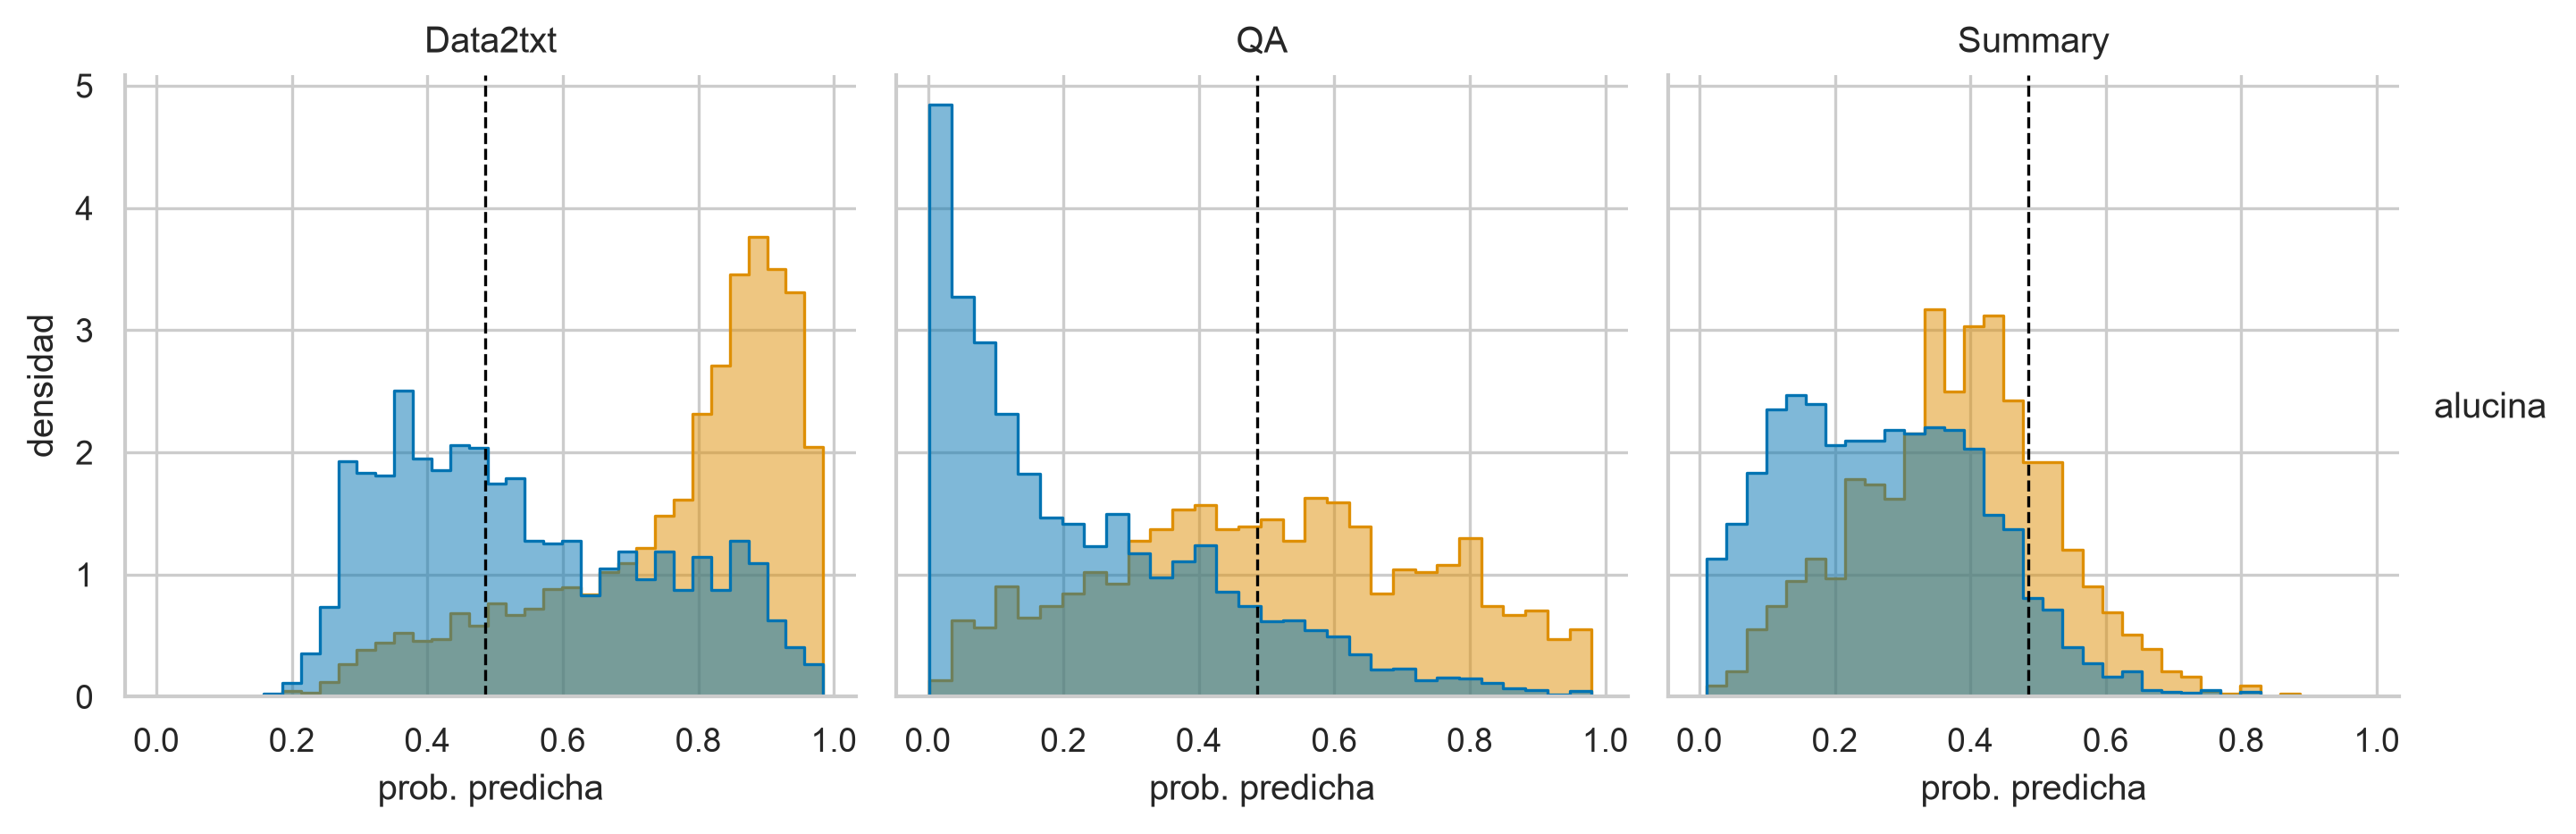
\includegraphics[width=\textwidth]{err_prob_por_tarea}
\caption{Probabilidad predicha por clase y tarea.}
\end{subfigure}\hfill
\begin{subfigure}{0.32\textwidth}
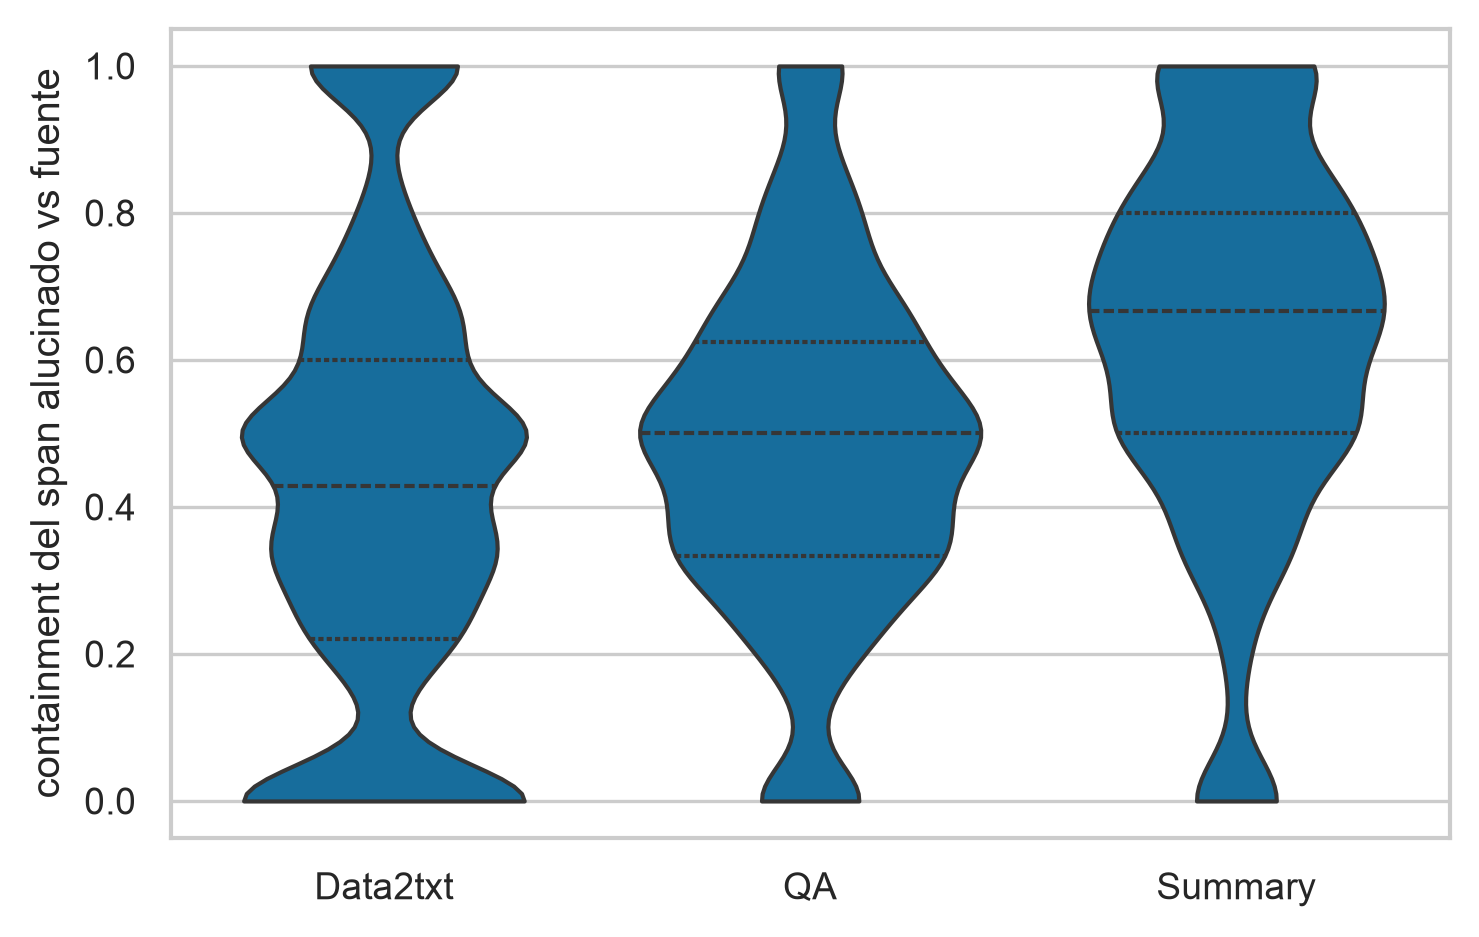
\includegraphics[width=\textwidth]{err_span_containment}
\caption{Solape del tramo alucinado por tarea.}
\end{subfigure}\hfill
\begin{subfigure}{0.32\textwidth}
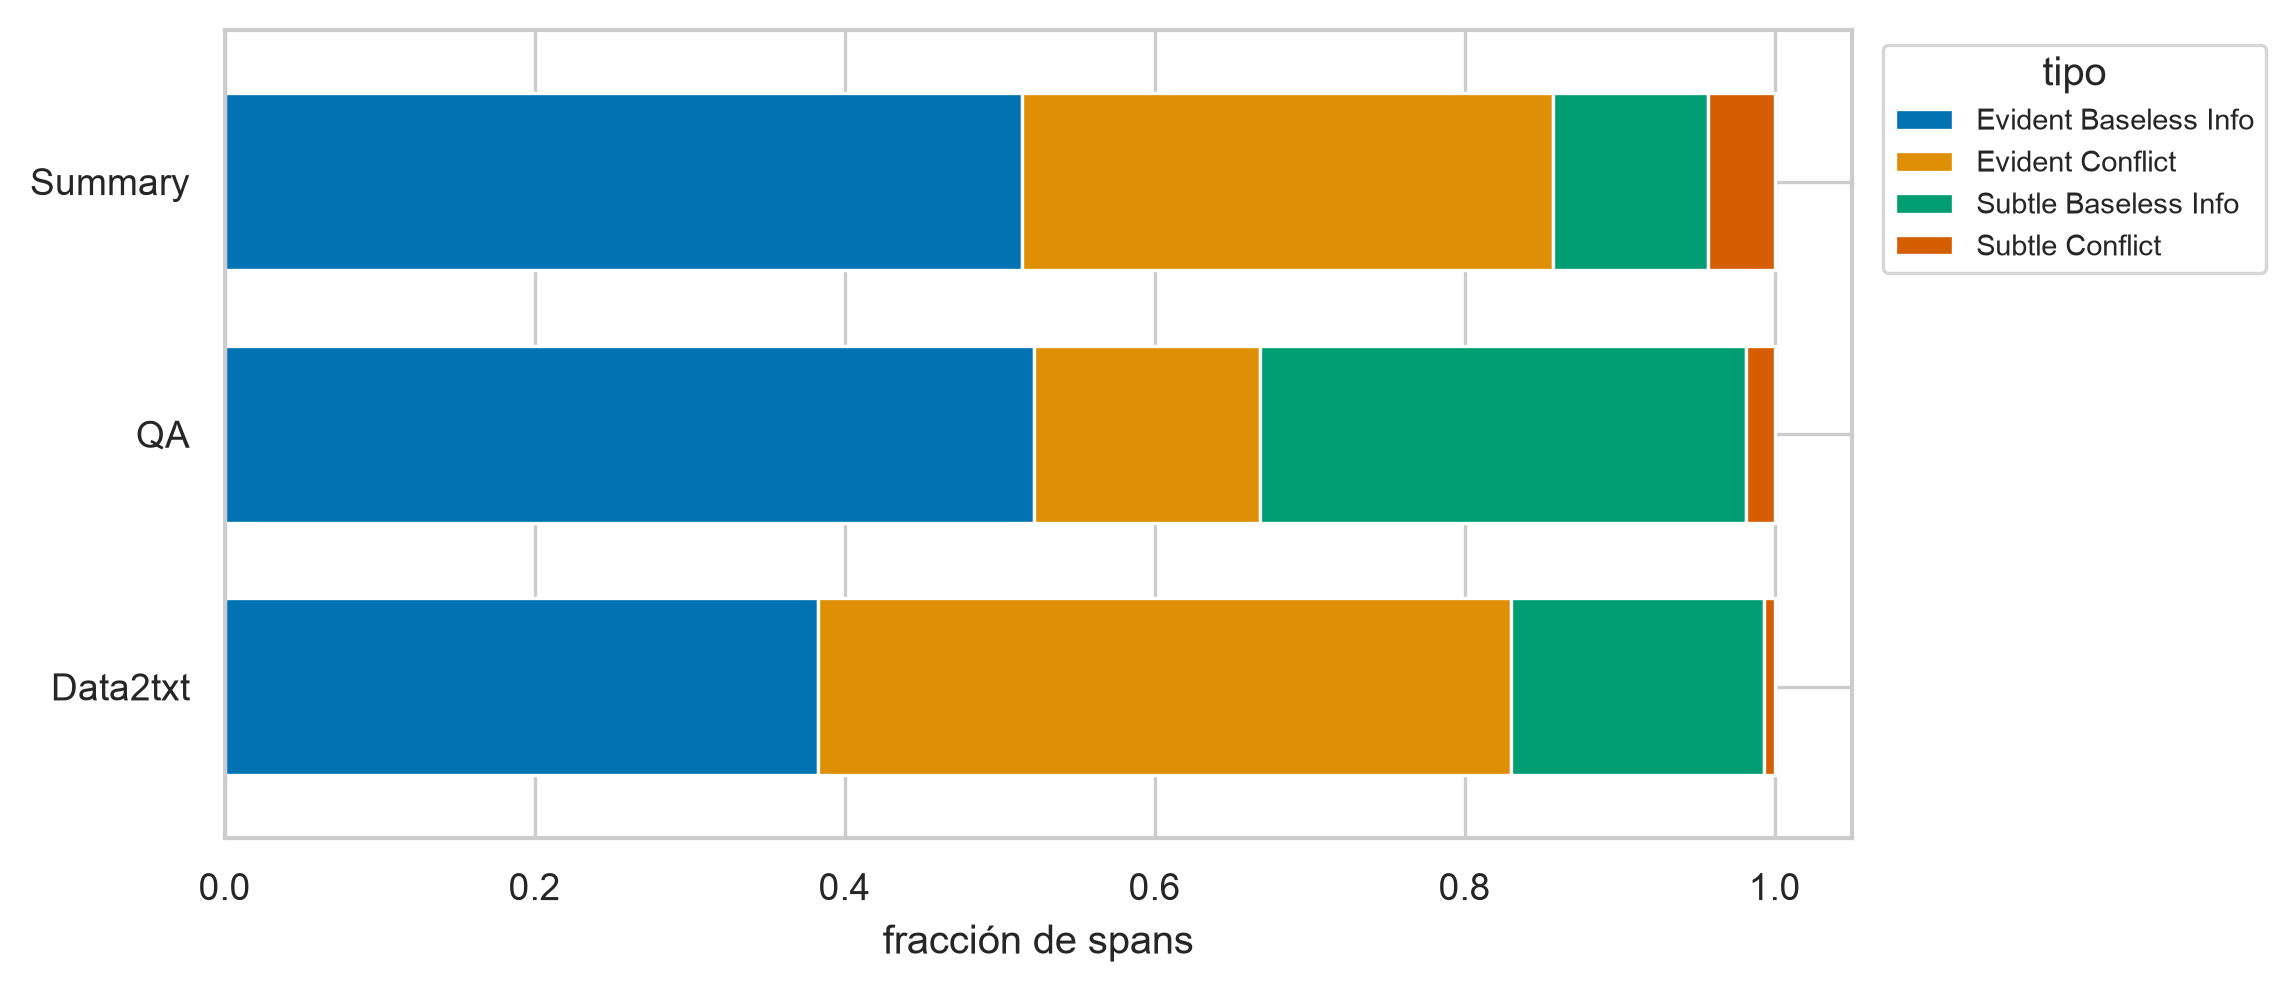
\includegraphics[width=\textwidth]{err_tipo_por_tarea}
\caption{Composición de tipos por tarea.}
\end{subfigure}
\caption{El cuello de botella de Summary es el camuflaje léxico, no el tipo de
alucinación. El tramo alucinado de un resumen comparte firma léxica con el texto fiel.}
\label{fig:err}
\end{figure}

\subsection{El umbral de decisión}

Si una parte de los falsos negativos es cuestión de umbral, la primera palanca es el
umbral mismo. Comparamos tres criterios, todos con los umbrales fijados en el
entrenamiento y aplicados al test: el índice de Youden global, que es el criterio de
partida; el máximo de F1 por tarea; y el máximo de F2 por tarea, que pondera el recall
cuatro veces más que la precisión y penaliza el falso negativo. El
Cuadro~\ref{tab:umbral} recoge el efecto por tarea, y la Figura~\ref{fig:barrido}
muestra cómo cada métrica cambia al mover el umbral.

\begin{table}[H]
\centering
\small
\begin{tabular}{llccccc}
\toprule
Estrategia & ámbito & F1 & precisión & recall & accuracy & FN \\
\midrule
Youden global & Global (pooled) & 0,682 & 0,684 & 0,680 & 0,779 & 302 \\
 & Data2txt & 0,821 & 0,765 & 0,884 & 0,751 & 67 \\
 & QA & 0,513 & 0,486 & 0,544 & 0,817 & 73 \\
 & Summary & 0,287 & 0,472 & 0,206 & 0,768 & 162 \\
\midrule
Por tarea (max-F1) & Global (pooled) & 0,656 & 0,547 & 0,821 & 0,700 & \textbf{169} \\
 & Data2txt & 0,821 & 0,766 & 0,884 & 0,752 & 67 \\
 & QA & 0,492 & 0,357 & 0,794 & 0,709 & \textbf{33} \\
 & Summary & \textbf{0,453} & 0,344 & 0,662 & 0,638 & \textbf{69} \\
\midrule
Por tarea (max-F2) & Global (pooled) & 0,577 & 0,409 & 0,982 & 0,497 & 17 \\
 & Data2txt & 0,786 & 0,648 & 1,000 & 0,650 & 0 \\
 & QA & 0,391 & 0,244 & 0,981 & 0,457 & 3 \\
 & Summary & 0,407 & 0,261 & 0,931 & 0,386 & 14 \\
\bottomrule
\end{tabular}
\caption{Estrategias de umbral sobre el test oficial. El umbral por tarea recupera el
44\,\% de los falsos negativos (de 302 a 169) y triplica el recall de Summary, a costa
de precisión. F2 lleva el recall casi a uno pero hunde la accuracy.}
\label{tab:umbral}
\end{table}

\begin{figure}[H]
\centering
\begin{subfigure}{0.48\textwidth}
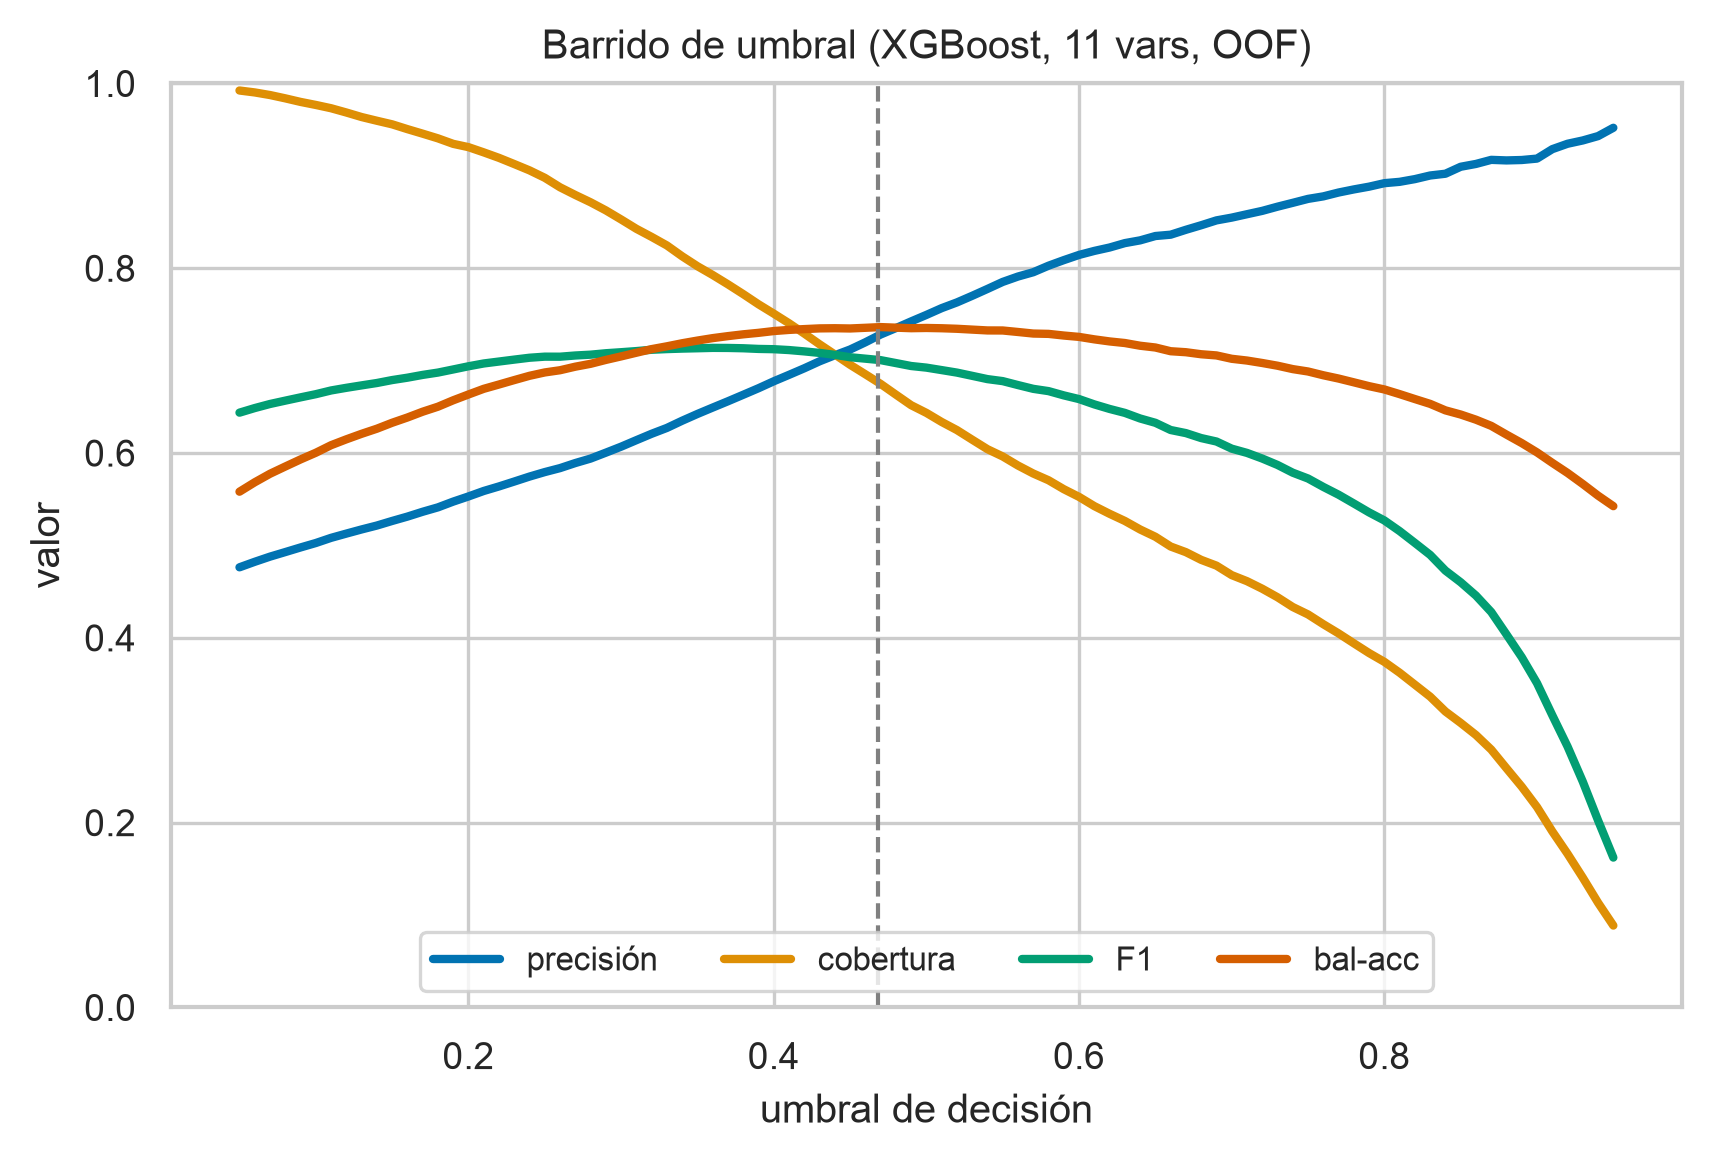
\includegraphics[width=\textwidth]{desb_barrido_umbral}
\caption{Barrido de umbral (OOF de train).}
\label{fig:barrido}
\end{subfigure}\hfill
\begin{subfigure}{0.48\textwidth}
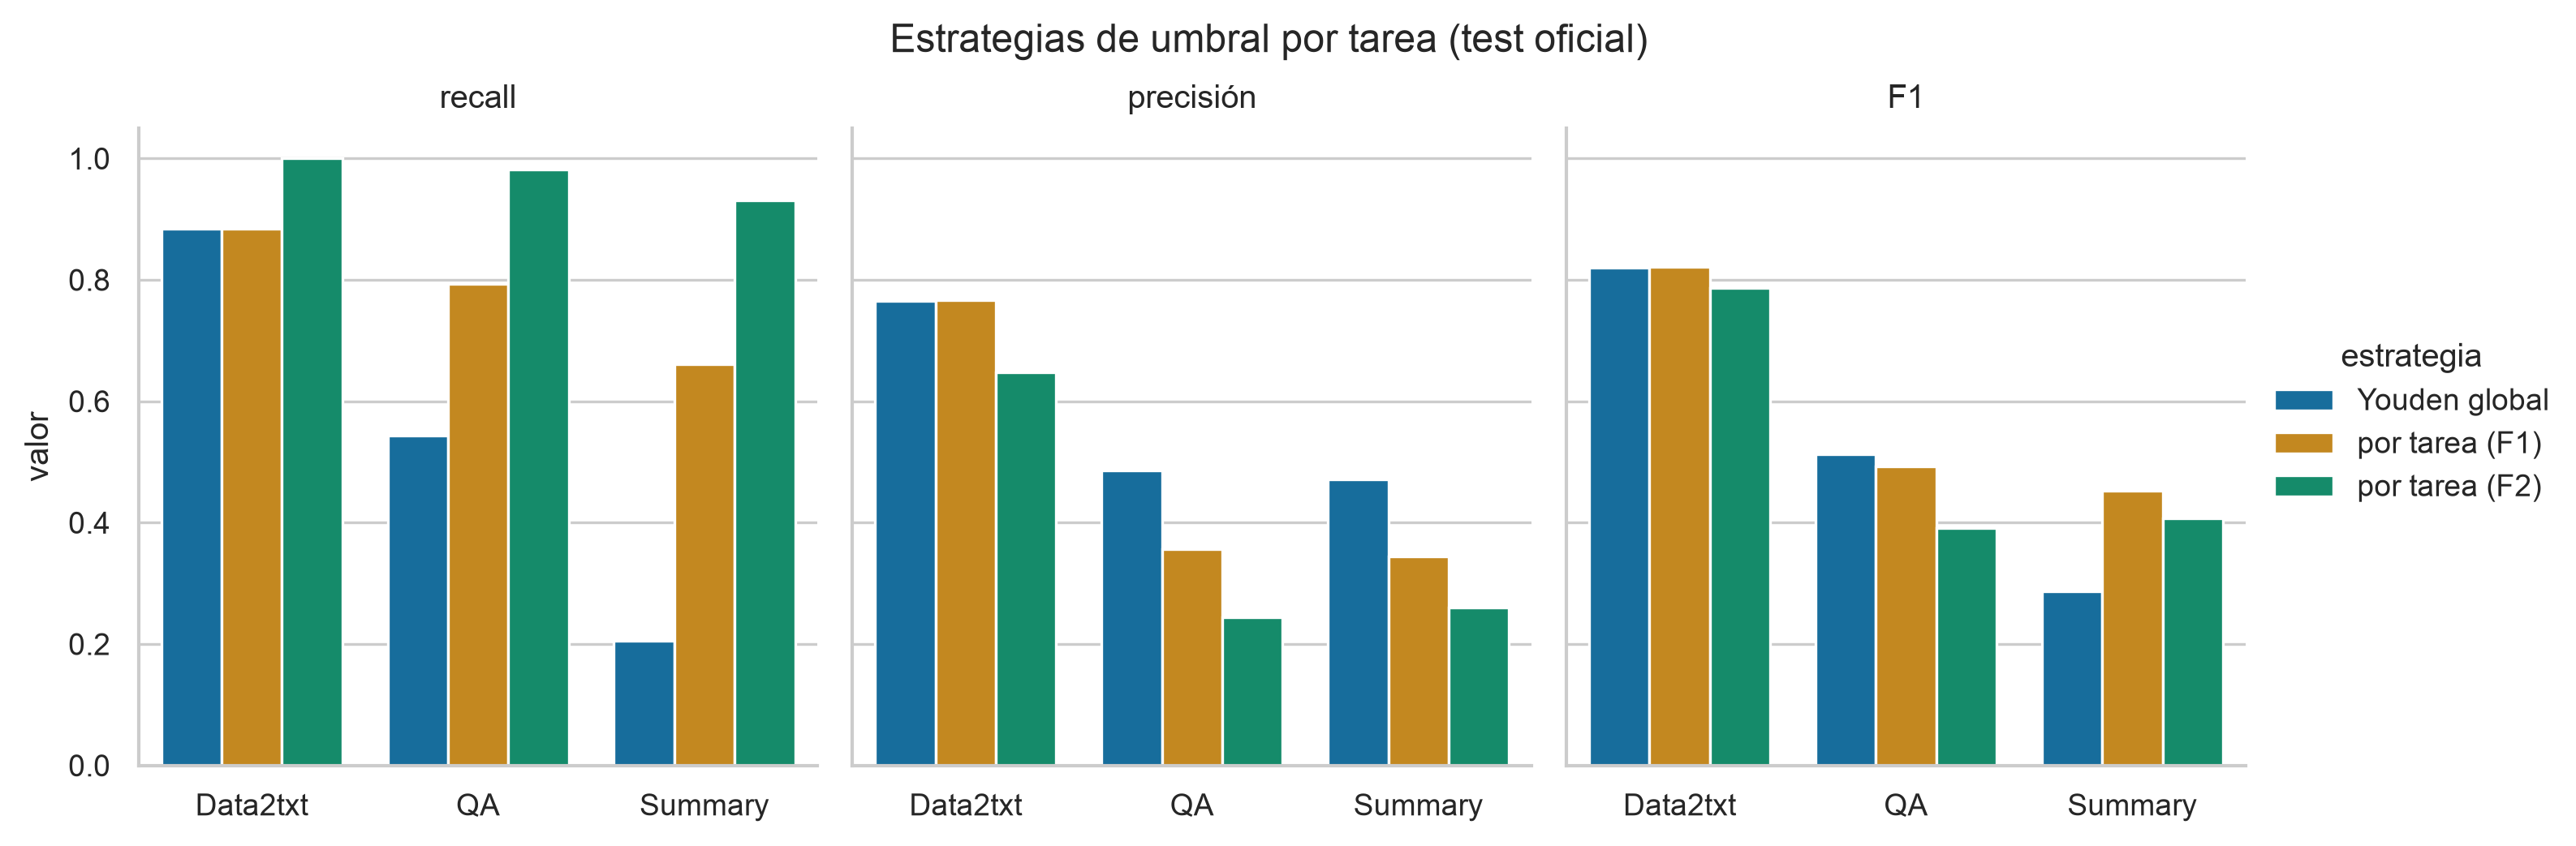
\includegraphics[width=\textwidth]{desb_estrategias_umbral}
\caption{Estrategias por tarea (test).}
\end{subfigure}
\caption{El umbral desliza el punto de operación entre precisión y recall. Un umbral por
tarea reconoce que cada tarea tiene una prevalencia distinta.}
\end{figure}

El F1 global admite dos lecturas que conviene separar. El F1 \emph{pooled}, calculado
sobre todas las respuestas juntas, baja con el umbral por tarea, de 0,682 a 0,656, porque
la caída de precisión pesa en el agregado. El F1 \emph{macro}, media de los tres F1 por
tarea, sube de 0,540 a 0,589, porque recompensa la mejora en Summary. Reportamos los dos:
el pooled es el que suele dar la literatura, y el macro refleja mejor la mejora donde
importa.

Aquí surge una tentación que conviene desmentir. Fijar el umbral por máximo de F1 no da
un premio gratis en el agregado: el máximo de F1 global fijado en entrenamiento
generaliza peor al test que Youden, porque la prevalencia de entrenamiento (0,445) no es
la del test (0,349), y el umbral bajo que maximiza F1 en entrenamiento resulta demasiado
agresivo fuera. La ganancia real del umbral por tarea no es en F1 pooled, sino en recall
y en el F1 de la tarea difícil.

\subsection{Corrección de prior de Saerens}

Si el problema de QA es que la prevalencia del test difiere de la del entrenamiento, un
remedio más principiado que mover el umbral a mano es corregir el prior. El método de
Saerens \cite{saerens2002} estima la prevalencia del test sin usar sus etiquetas, por un
procedimiento de esperanza-maximización sobre los propios scores, y reajusta el posterior
del clasificador a esa prevalencia. Lo probamos sobre probabilidades ya calibradas por
regresión isotónica.

El método colapsa. La estimación por esperanza-maximización converge a priores
degenerados: 1,000 en Data2txt, 0,000 en QA y 0,000 en Summary, frente a los reales
0,643, 0,178 y 0,227 (Figura~\ref{fig:saerens}). Con priores 0 y 1 la decisión se vuelve
trivial, todo alucinado en Data2txt y nada en QA ni Summary. La causa es que las
distribuciones de score de las dos clases se solapan demasiado, sobre todo en Summary,
para que el procedimiento identifique la proporción de mezcla. La vía queda descartada
con evidencia.

\begin{figure}[H]
\centering
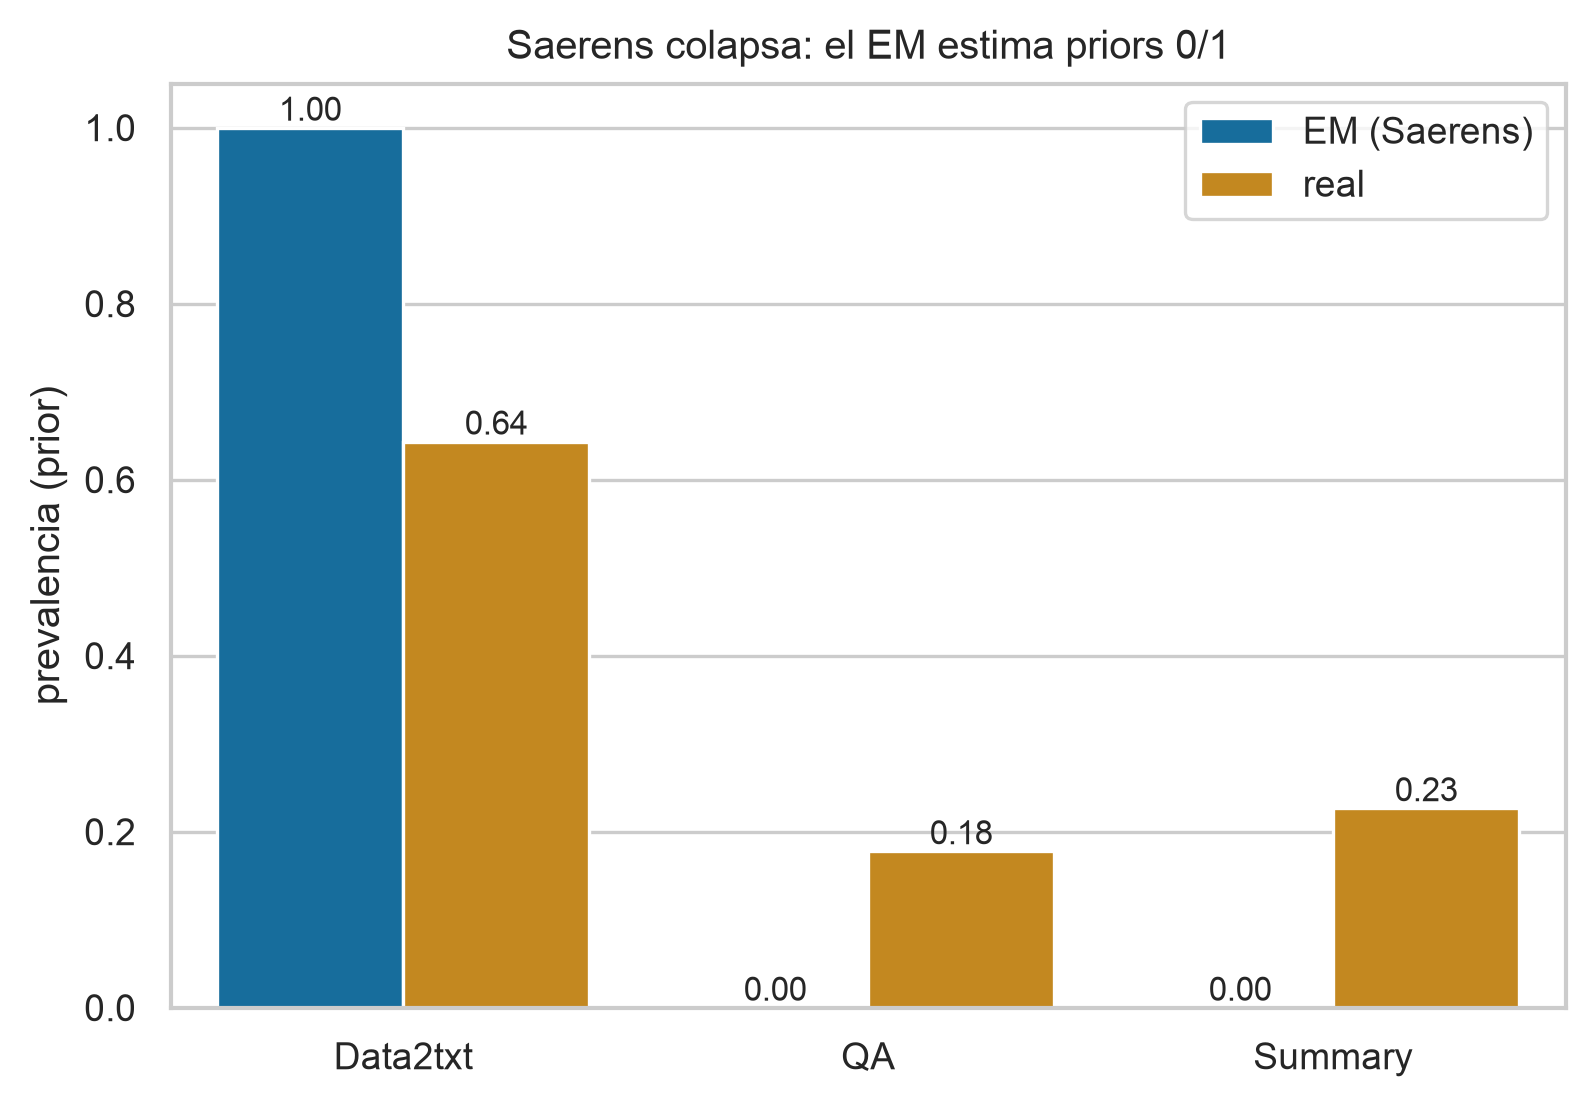
\includegraphics[width=0.7\textwidth]{desb_saerens_colapso}
\caption{Corrección de prior de Saerens. El prior estimado por esperanza-maximización
colapsa a 0 o 1 y no recupera la prevalencia real. Resultado negativo.}
\label{fig:saerens}
\end{figure}

\subsection{Remuestreo y aprendizaje sensible al coste}

Queda la idea más intuitiva: reequilibrar las clases antes de entrenar, igualando las
alucinaciones por tarea. Probamos sobremuestreo aleatorio, submuestreo aleatorio y
SMOTE \cite{chawla2002smote}, siempre por tarea y solo en entrenamiento, y también el
aprendizaje sensible al coste, que penaliza el falso negativo con un peso de clase. La
pregunta correcta no es qué le pasa al F1 a un umbral fijo, sino si el tratamiento mueve
la frontera, es decir, la separación real entre clases medida por el AUC-PR, que no
depende del umbral.

\begin{table}[H]
\centering
\begin{tabular}{lccc}
\toprule
Estrategia & Data2txt & QA & Summary \\
\midrule
Base (sin tratar) & 0,858 & 0,528 & 0,410 \\
Sobremuestreo por tarea & 0,853 & 0,532 & 0,390 \\
Submuestreo por tarea & 0,854 & 0,543 & 0,409 \\
SMOTE por tarea & 0,855 & 0,533 & 0,357 \\
Sensible al coste & 0,857 & 0,528 & 0,403 \\
\bottomrule
\end{tabular}
\caption{AUC-PR por tarea según el tratamiento del desbalance en el entrenamiento.
Ninguna variante mueve la frontera; SMOTE la empeora en Summary. Reequilibrar clases no
crea señal.}
\label{tab:frontera}
\end{table}

El Cuadro~\ref{tab:frontera} y la Figura~\ref{fig:frontera} lo muestran sin ambigüedad:
la frontera por tarea no se mueve, y SMOTE la empeora en Summary. El AUC-PR global cae
con el remuestreo por tarea porque distorsiona la ordenación entre tareas. Lo que SMOTE
parece ganar a un umbral fijo, subir el recall de Summary, es un espejismo: entrena a
50/50, infla los scores y hace que el mismo umbral actúe como uno más bajo. El modelo
limpio con umbral por tarea lo domina, con mejor F1 de Summary (0,453 frente a 0,429),
menos falsos negativos y mejor frontera. La Figura~\ref{fig:fn} resume la comparación en
la moneda que nos importa, los falsos negativos totales.

\begin{figure}[H]
\centering
\begin{subfigure}{0.55\textwidth}
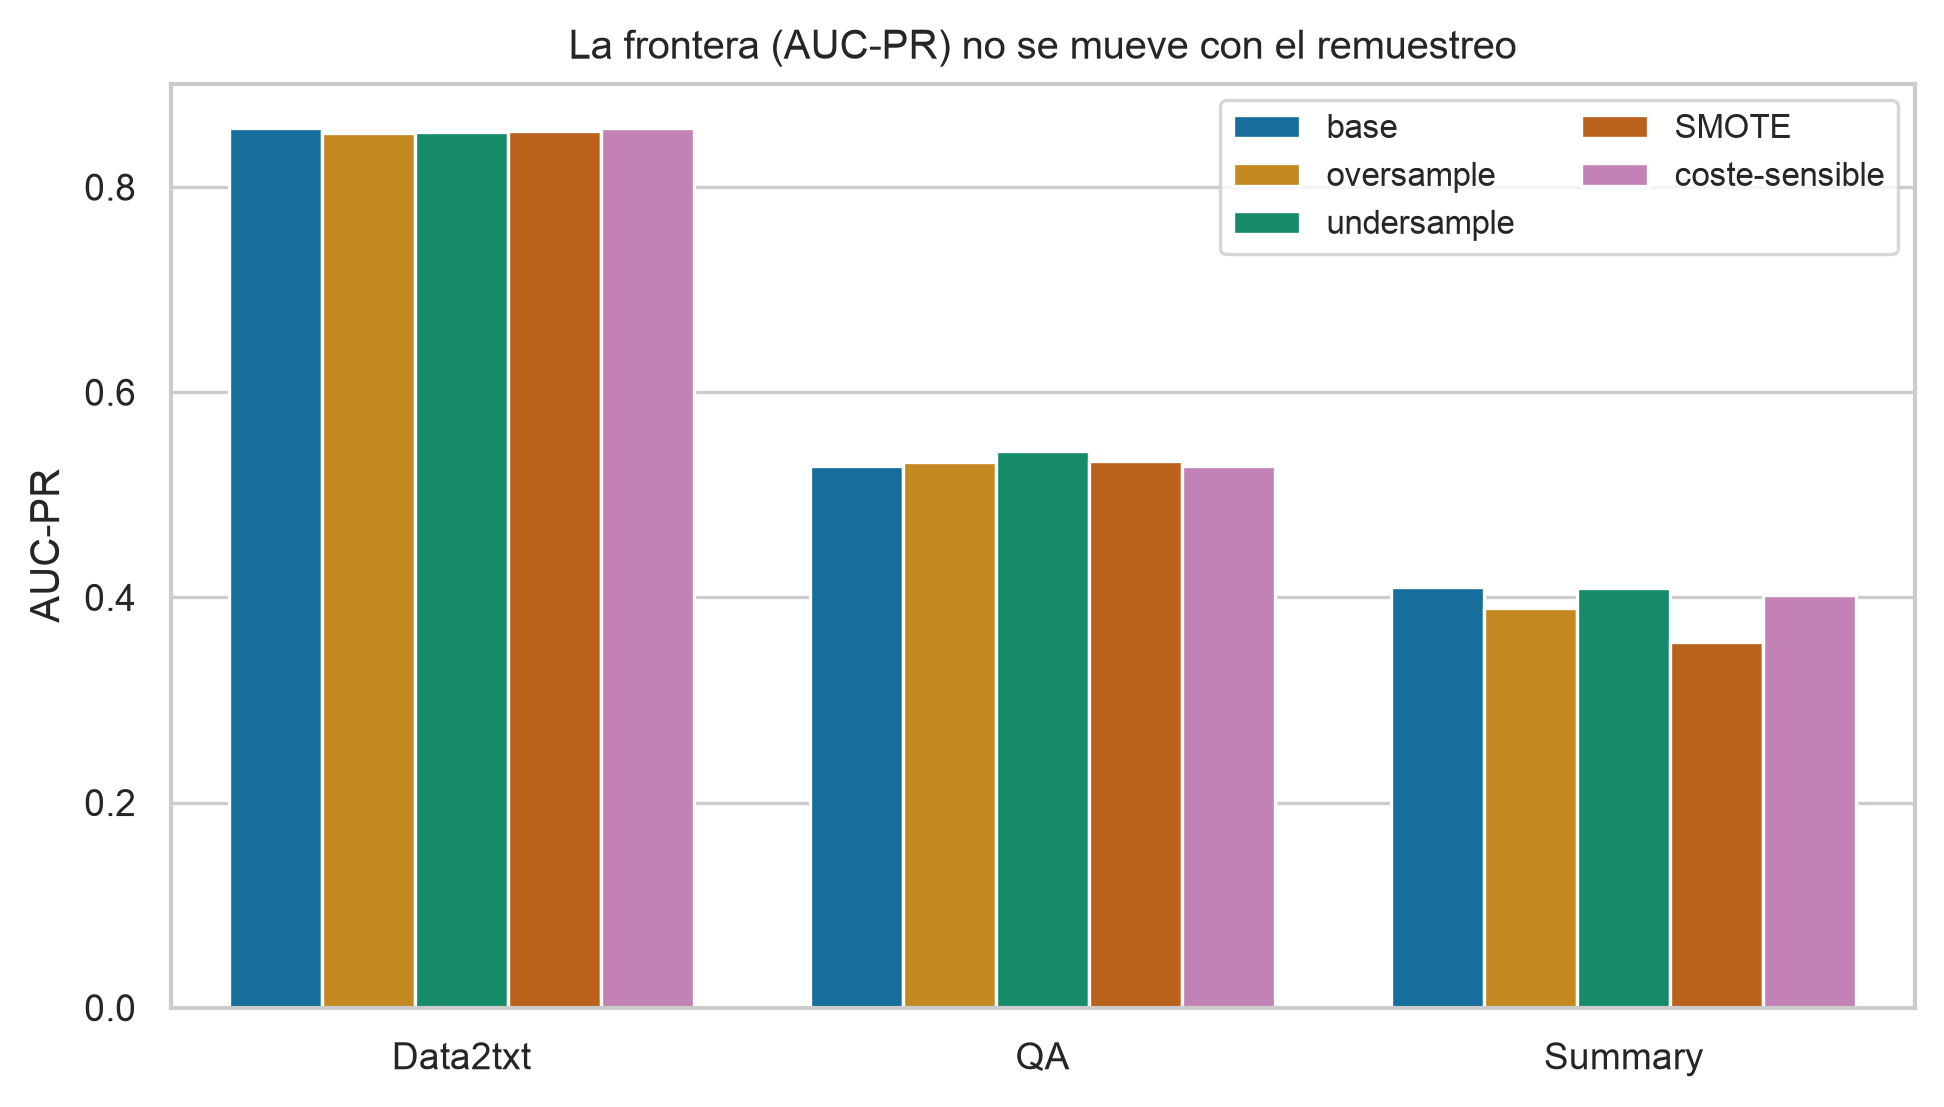
\includegraphics[width=\textwidth]{desb_frontera_remuestreo}
\caption{Frontera (AUC-PR) por estrategia.}
\label{fig:frontera}
\end{subfigure}\hfill
\begin{subfigure}{0.42\textwidth}
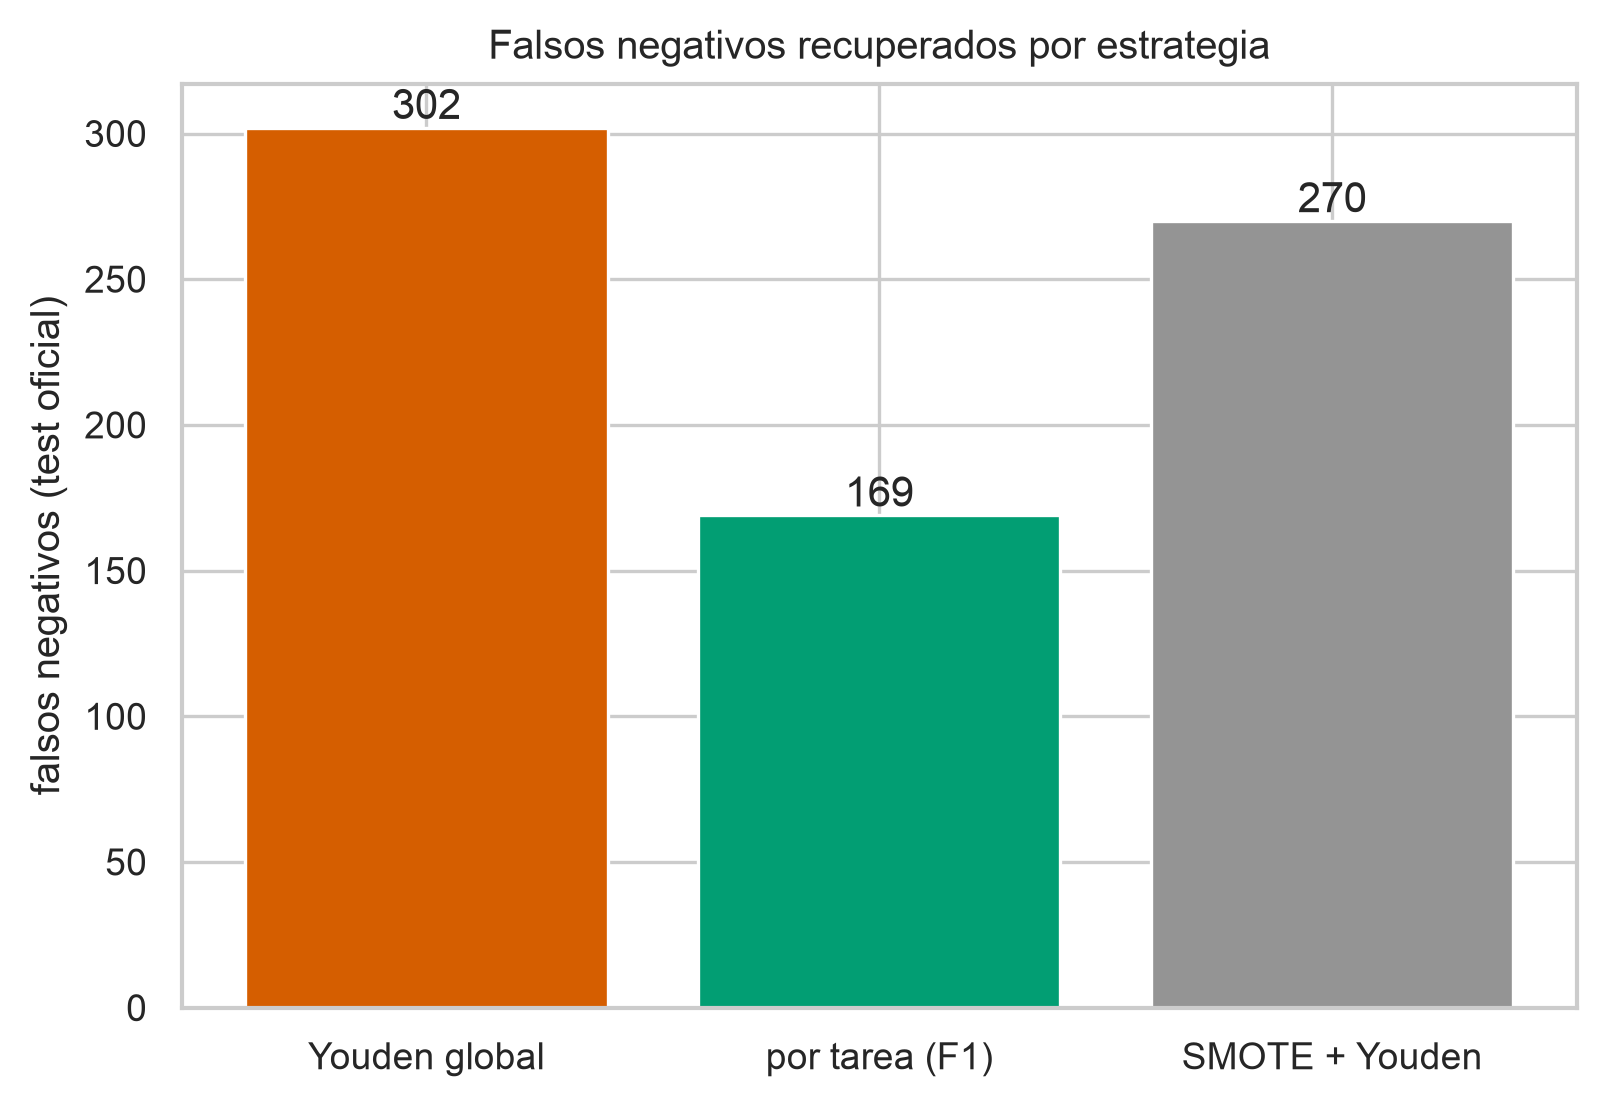
\includegraphics[width=\textwidth]{desb_fn_recuperados}
\caption{Falsos negativos totales.}
\label{fig:fn}
\end{subfigure}
\caption{El remuestreo no mueve la frontera. El umbral por tarea recupera más falsos
negativos que SMOTE, sobre una frontera mejor.}
\end{figure}

Las matrices de confusión por tarea (Figura~\ref{fig:conf}) cierran el argumento
visualmente: al pasar del umbral global al umbral por tarea, los falsos negativos de QA
bajan de 73 a 33 y los de Summary de 162 a 69, a cambio de más falsos positivos.

\begin{figure}[H]
\centering
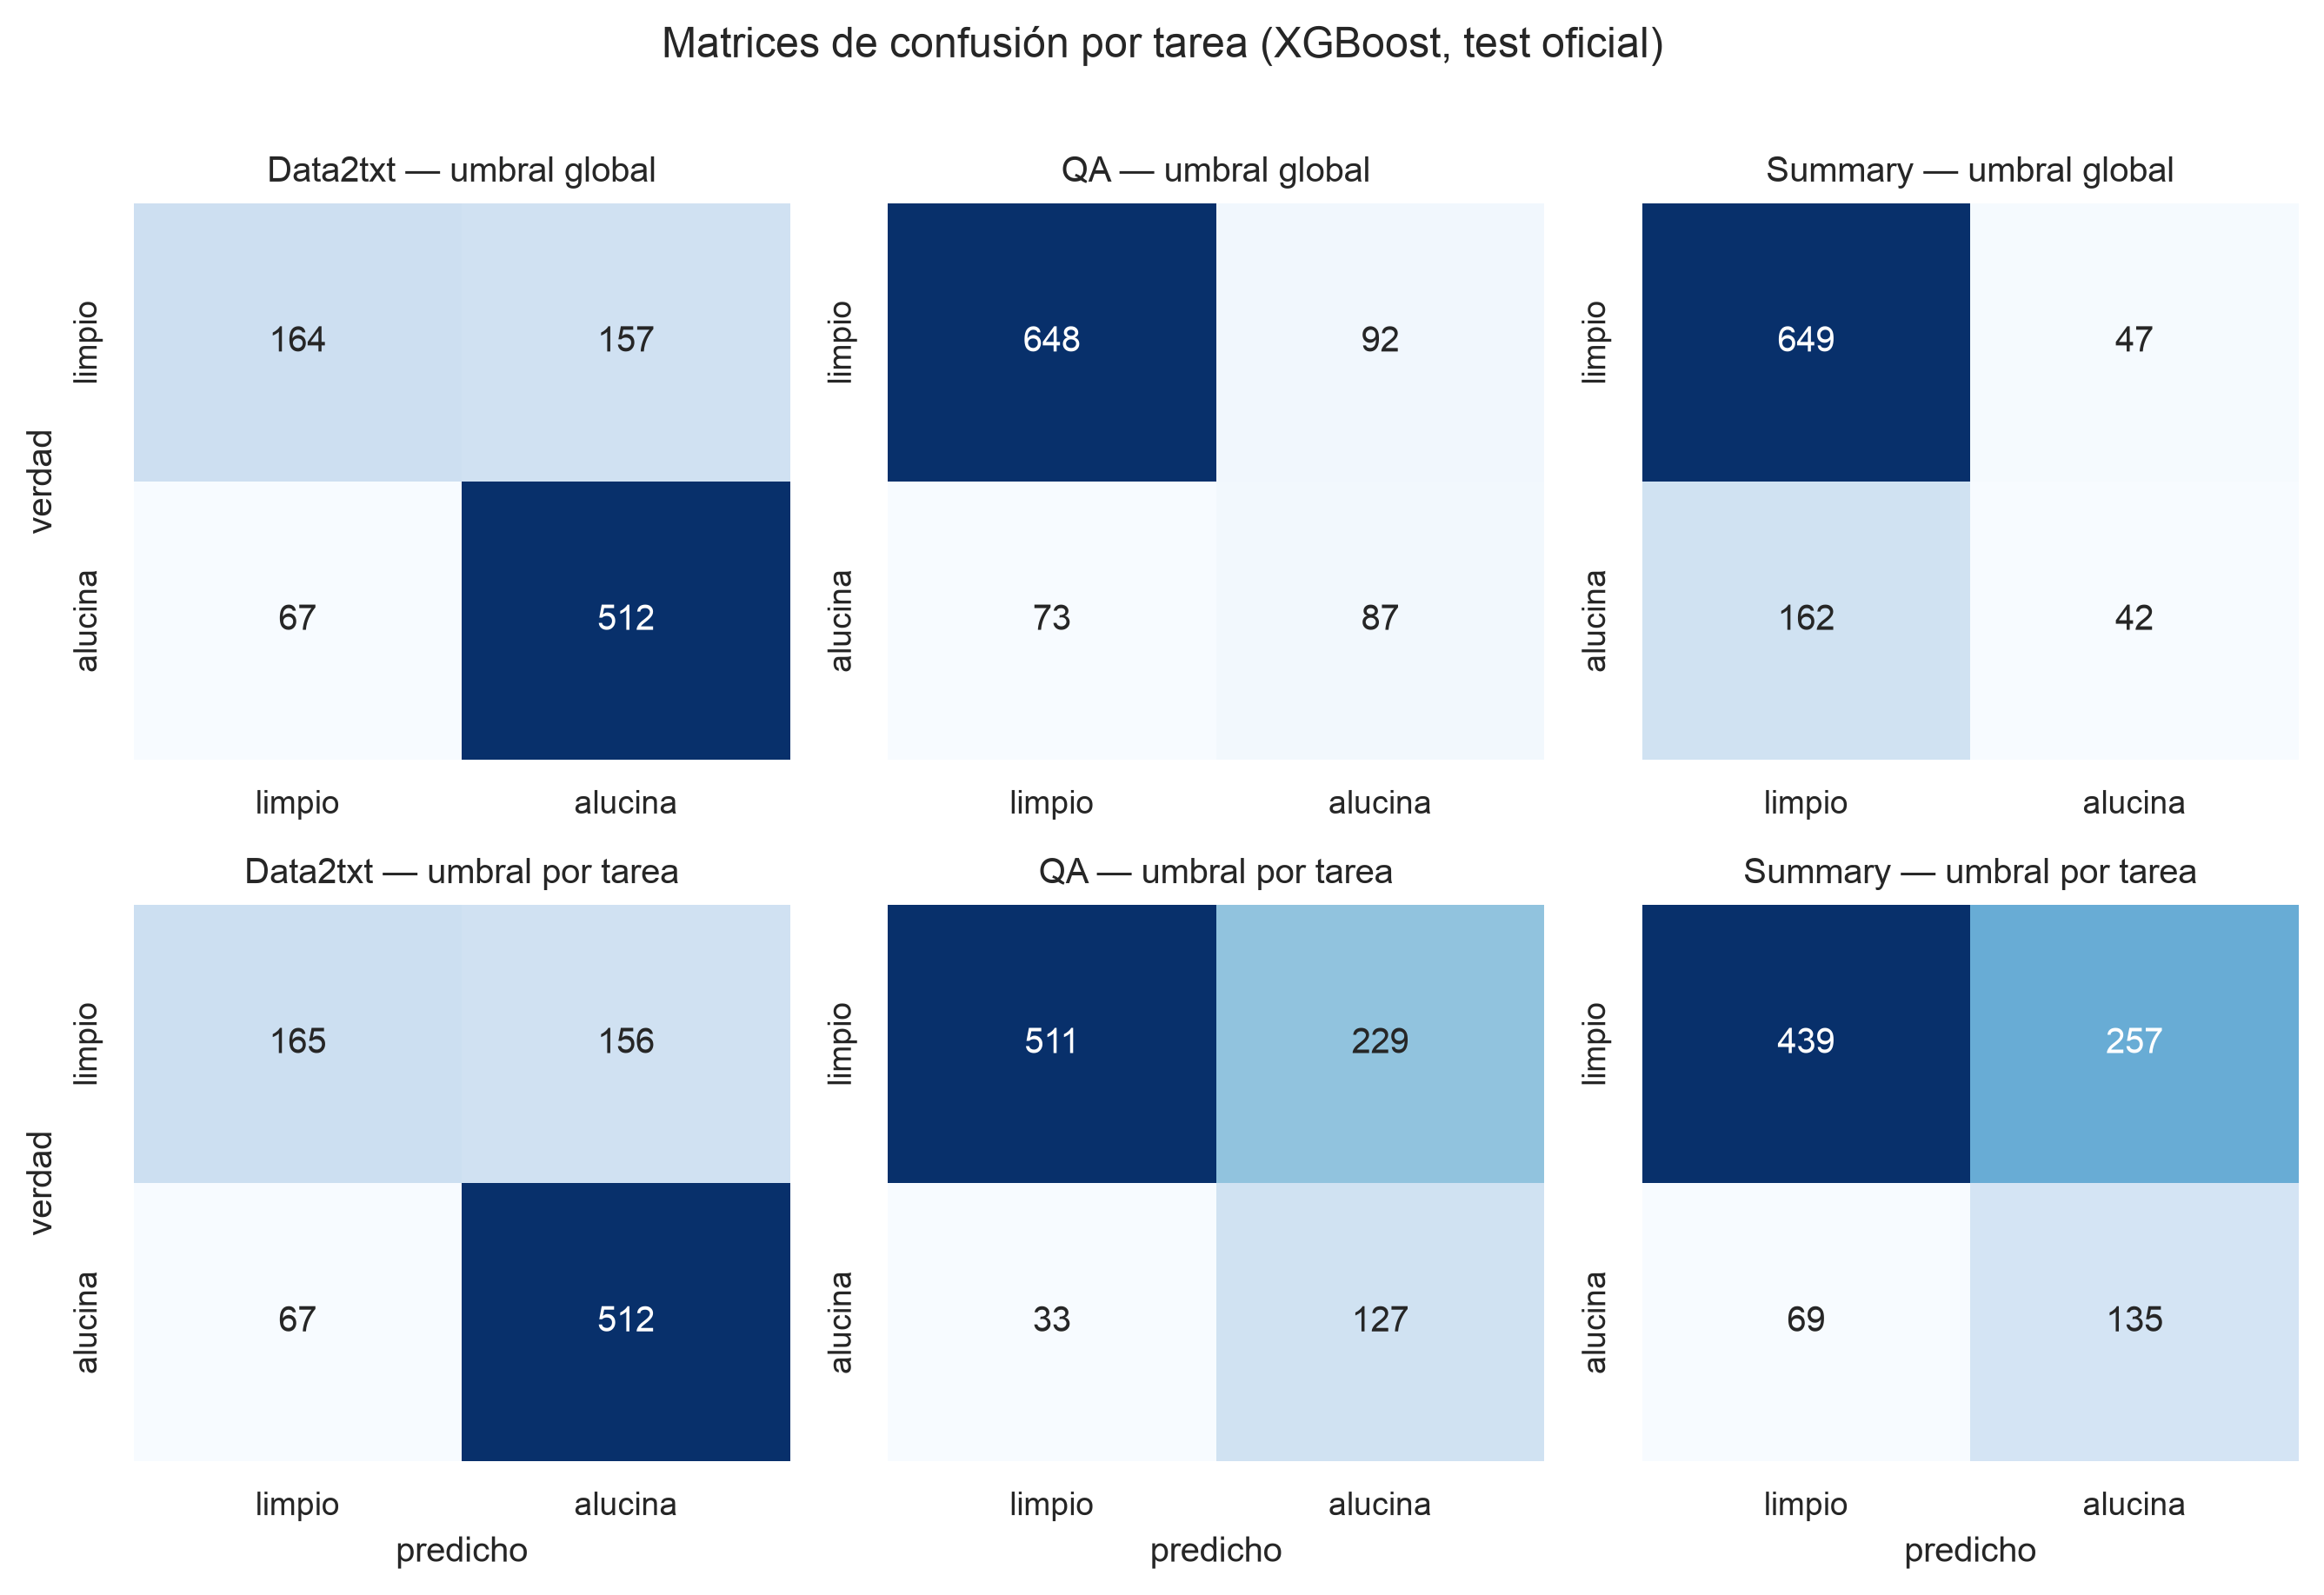
\includegraphics[width=\textwidth]{eval_confusion_por_tarea}
\caption{Matrices de confusión por tarea (XGBoost, test oficial). La fila superior usa
umbral global; la inferior, umbral por tarea. La diagonal de aciertos de alucinación
crece en QA y Summary.}
\label{fig:conf}
\end{figure}

\paragraph{Decisión.} Adoptamos como punto de operación el umbral por tarea que maximiza
F1, fijado en el entrenamiento. Es la única palanca honesta contra los falsos negativos:
recupera el 44\,\% de ellos y hace competitivo el F1 de Summary sin tocar las
características ni el modelo. Descartamos, con prueba, la corrección de prior de Saerens,
el remuestreo en sus tres variantes y el aprendizaje sensible al coste, porque no mueven
la frontera.

\section{Modelos y evaluación honesta}

Evaluamos cinco clasificadores clásicos: regresión logística \cite{cox1958logreg},
$k$ vecinos más cercanos \cite{cover1967knn}, máquina de vectores de soporte
\cite{cortes1995svm}, bosque aleatorio \cite{breiman2001rf} y gradient boosting sobre
árboles \cite{friedman2001gbm,chen2016xgboost}. Cada uno se ajusta por búsqueda en
rejilla con \texttt{GroupKFold}, y se evalúa sobre el test oficial. El
Cuadro~\ref{tab:modelos} recoge las métricas por secciones, con el umbral por Youden y el
intervalo de confianza del AUC por bootstrap \cite{efron1979bootstrap}.

\begin{table}[H]
\centering
\small
\begin{tabular}{lccccccc}
\toprule
Modelo & AUC-ROC & IC 95\,\% & AUC-PR & F1 & precisión & recall & ECE \\
\midrule
Random Forest & \textbf{0,836} & [0,820, 0,851] & 0,745 & 0,680 & 0,651 & 0,710 & 0,069 \\
XGBoost & 0,835 & [0,819, 0,849] & 0,748 & 0,684 & 0,698 & 0,671 & \textbf{0,063} \\
KNN & 0,826 & [0,810, 0,841] & 0,735 & 0,678 & 0,628 & 0,737 & 0,065 \\
SVM & 0,819 & [0,801, 0,837] & 0,732 & \textbf{0,692} & 0,700 & 0,685 & 0,068 \\
Regresión logística & 0,816 & [0,800, 0,832] & 0,711 & 0,670 & 0,643 & 0,700 & 0,111 \\
\bottomrule
\end{tabular}
\caption{Comparativa de los cinco modelos en el test oficial (umbral por Youden). El AUC
supera el umbral 0,80 de la hipótesis. XGBoost combina buen AUC con la mejor calibración.}
\label{tab:modelos}
\end{table}

Los cinco modelos superan el umbral 0,80 de la hipótesis falsable. Las diferencias entre
ellos son pequeñas y sus intervalos de confianza se solapan. Elegimos XGBoost como
modelo de referencia porque combina un AUC entre los mejores con la mejor calibración,
medida por el error de calibración esperado. Las curvas ROC y precisión-recall, tanto en
validación cruzada como en el test oficial, aparecen en la Figura~\ref{fig:roc}.

\begin{figure}[H]
\centering
\begin{subfigure}{0.48\textwidth}
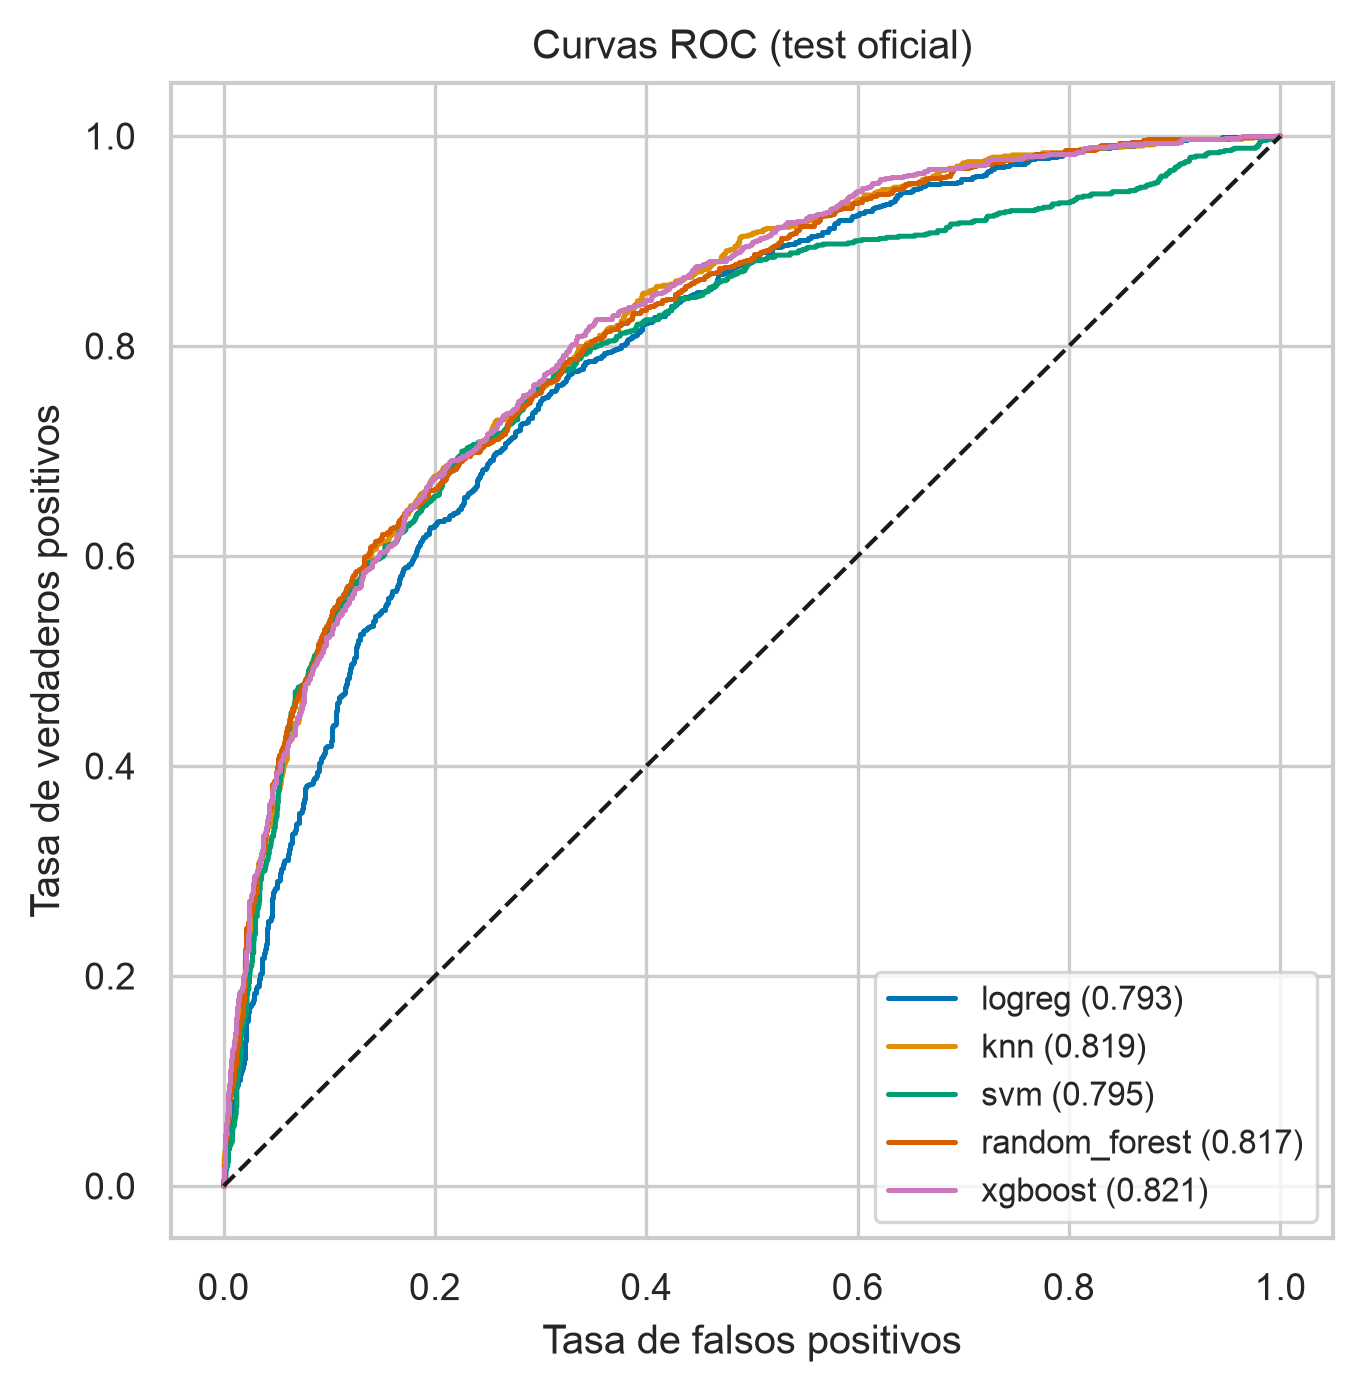
\includegraphics[width=\textwidth]{roc_test}
\caption{Curvas ROC (test oficial).}
\end{subfigure}\hfill
\begin{subfigure}{0.48\textwidth}
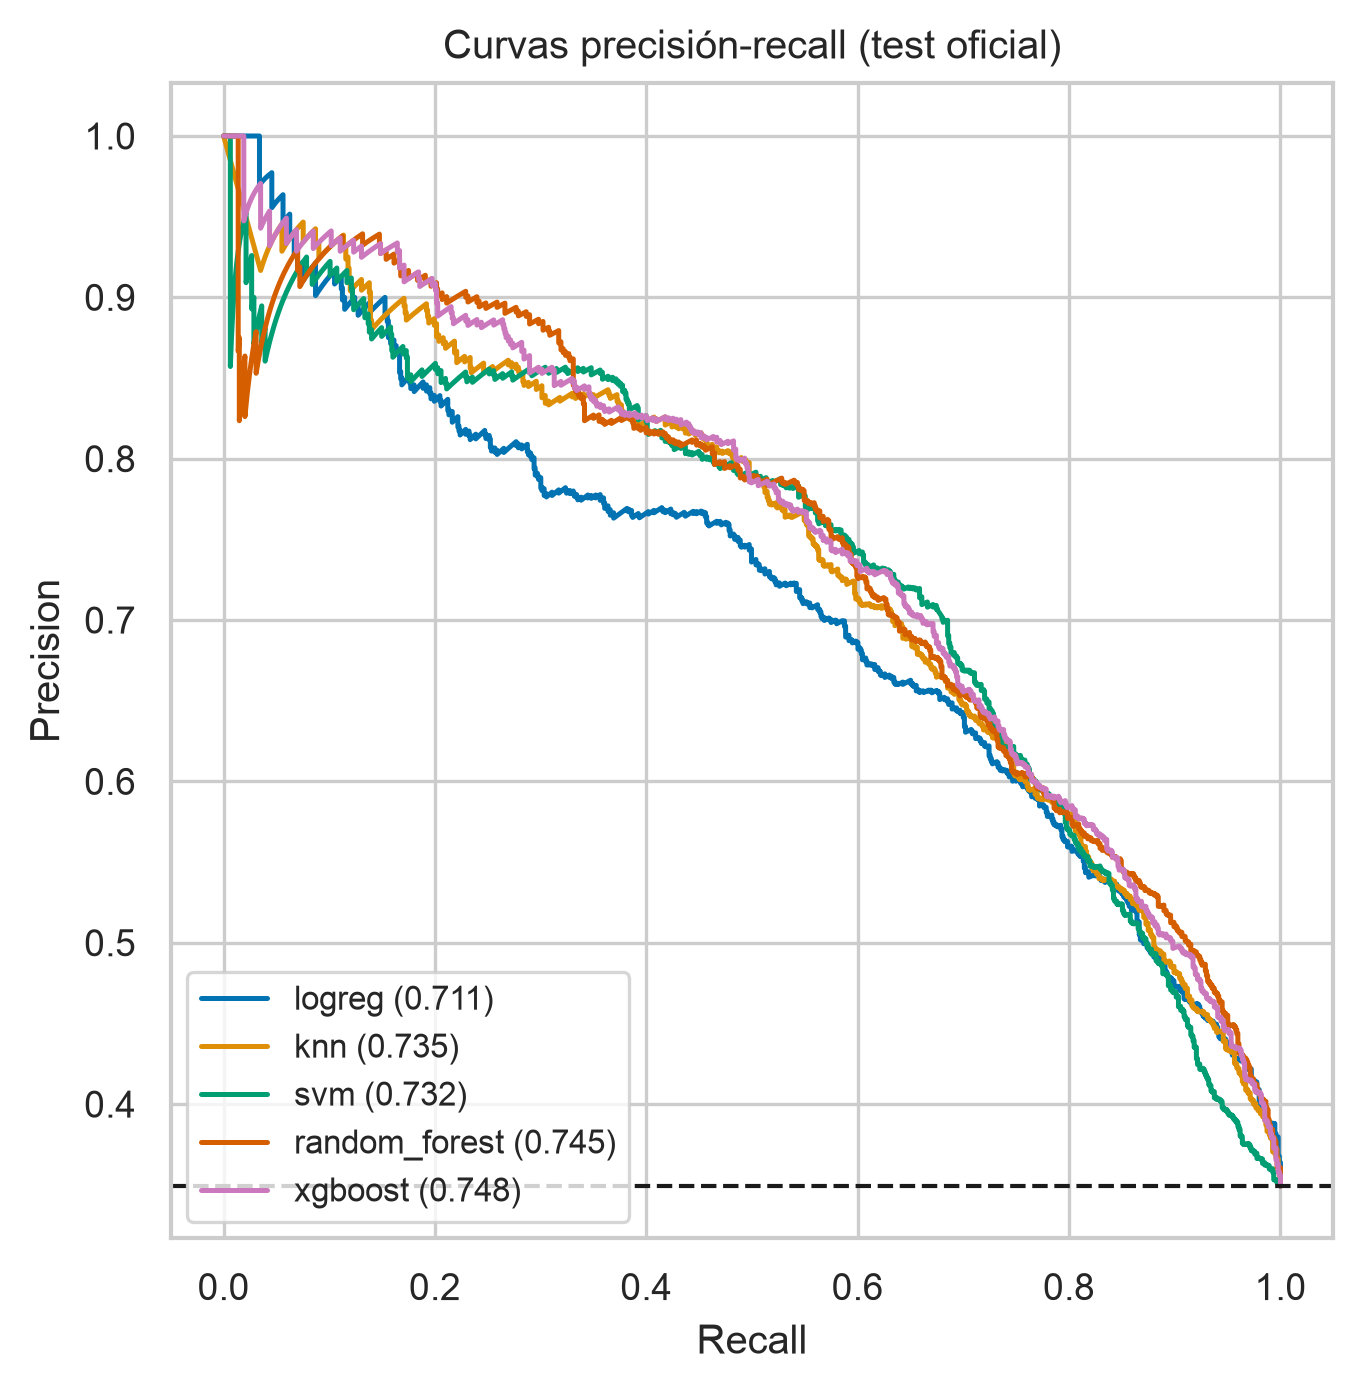
\includegraphics[width=\textwidth]{pr_test}
\caption{Curvas precisión-recall (test oficial).}
\end{subfigure}
\caption{Discriminación de los cinco modelos sobre el test oficial.}
\label{fig:roc}
\end{figure}

El desglose por tarea (Figura~\ref{fig:roctask}) confirma el diagnóstico: Data2txt y QA
se separan bien, con AUC en torno a 0,78 y 0,82, mientras Summary se queda en 0,70. La
paradoja de que QA tenga el mejor AUC y a la vez un F1 modesto se explica por la
prevalencia, no por la separación. La calibración
(Figura~\ref{fig:calib}) es razonable en crudo y mejora con regresión isotónica
\cite{platt1999}, lo que da probabilidades fiables para fijar el umbral.

\begin{figure}[H]
\centering
\begin{subfigure}{0.48\textwidth}
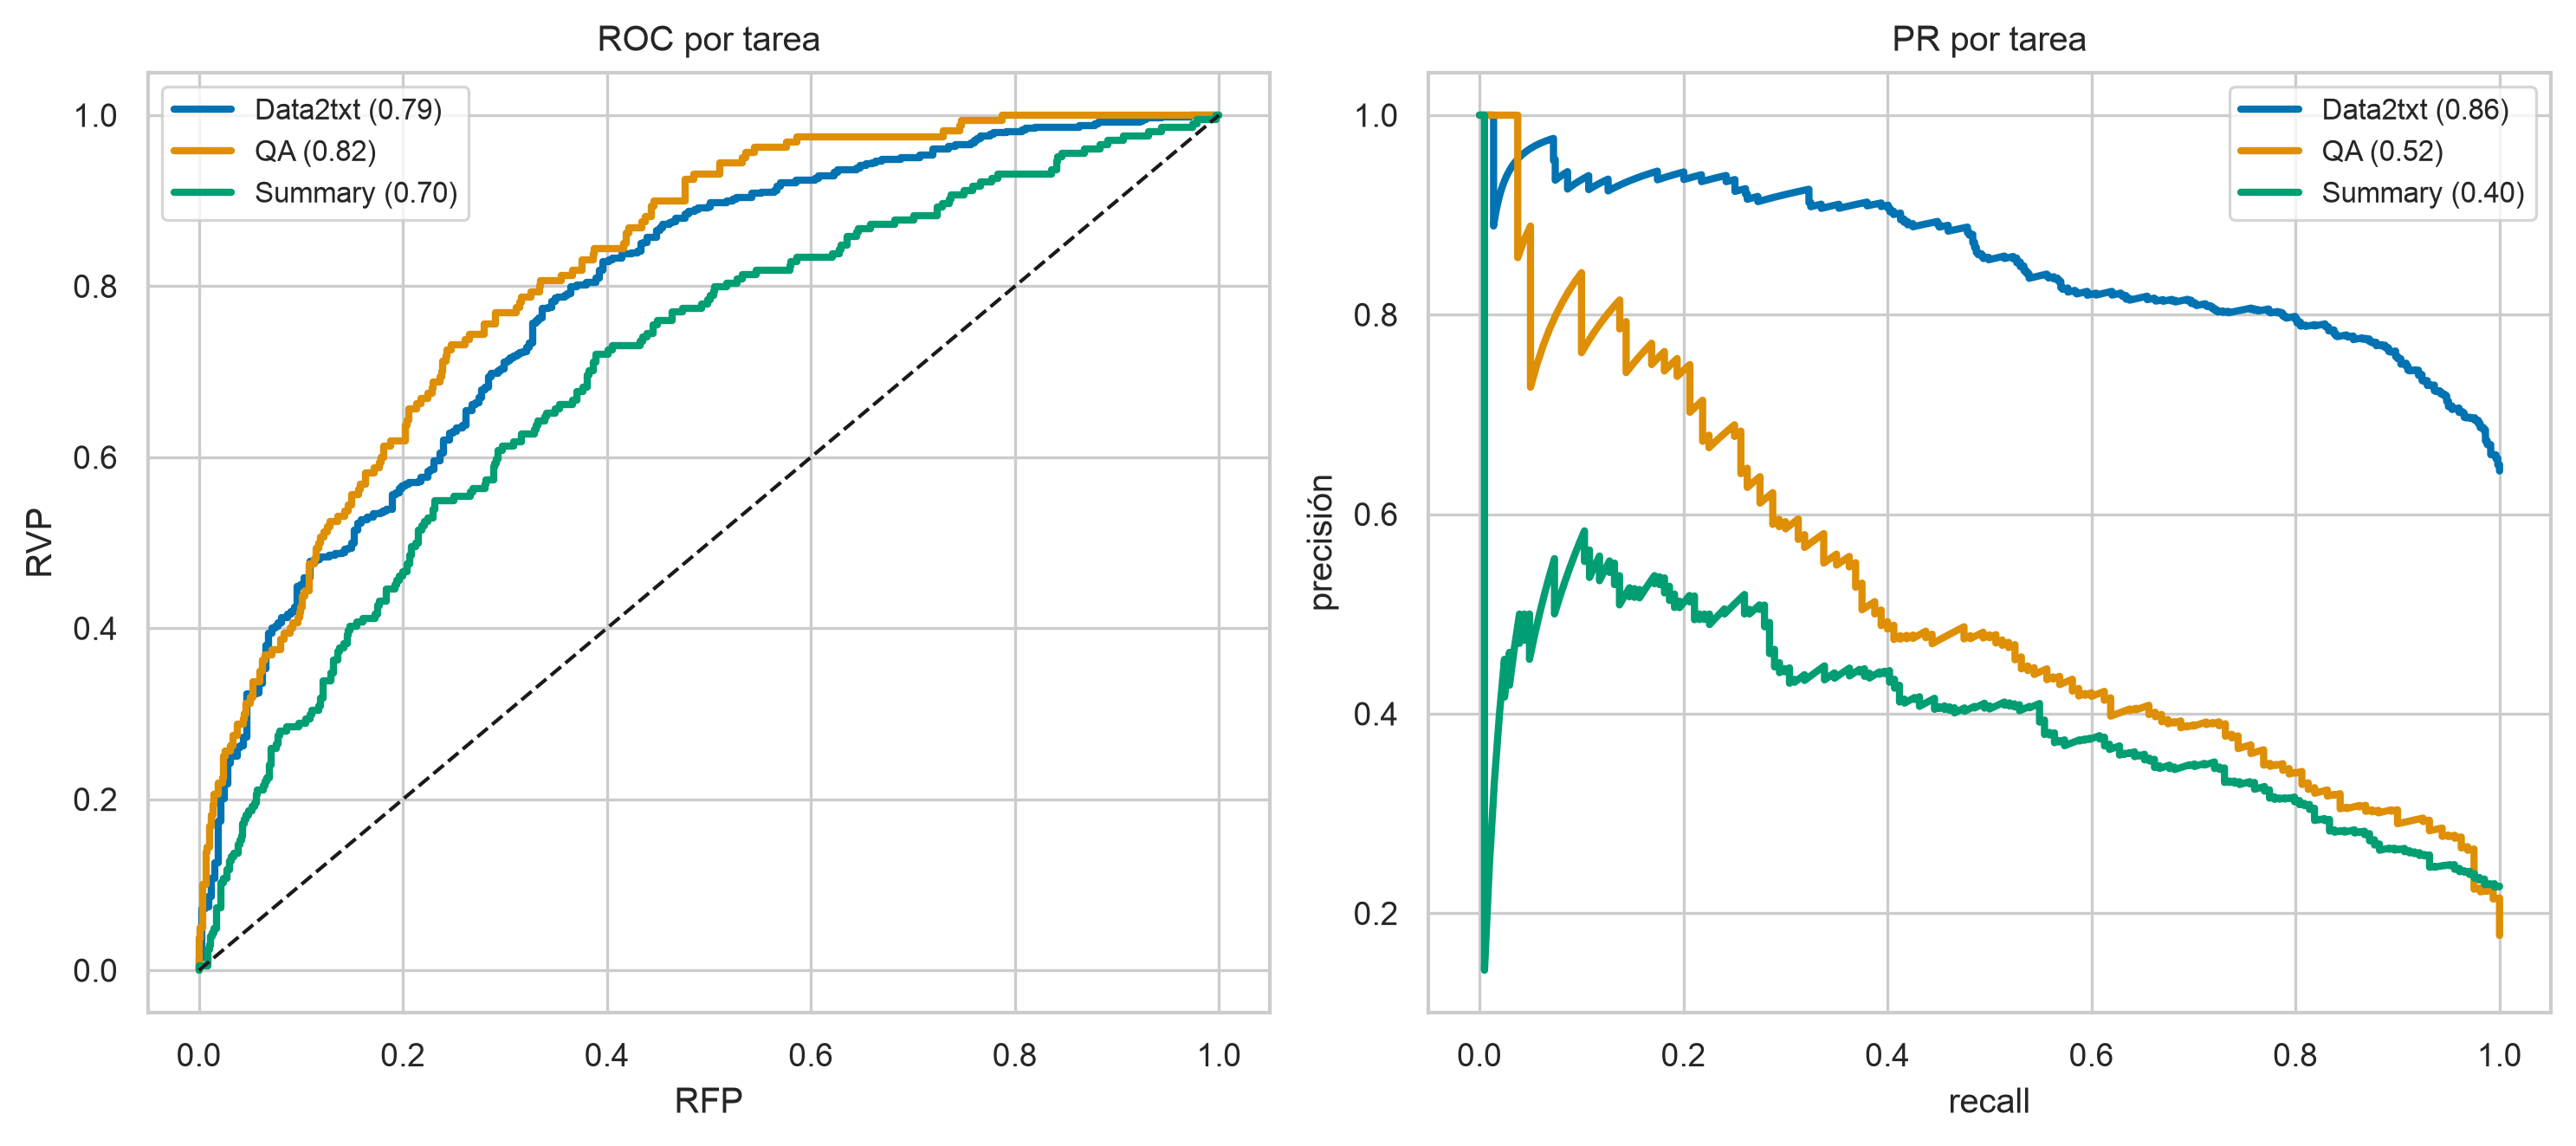
\includegraphics[width=\textwidth]{eval_roc_pr_por_tarea}
\caption{ROC y precisión-recall por tarea.}
\label{fig:roctask}
\end{subfigure}\hfill
\begin{subfigure}{0.48\textwidth}
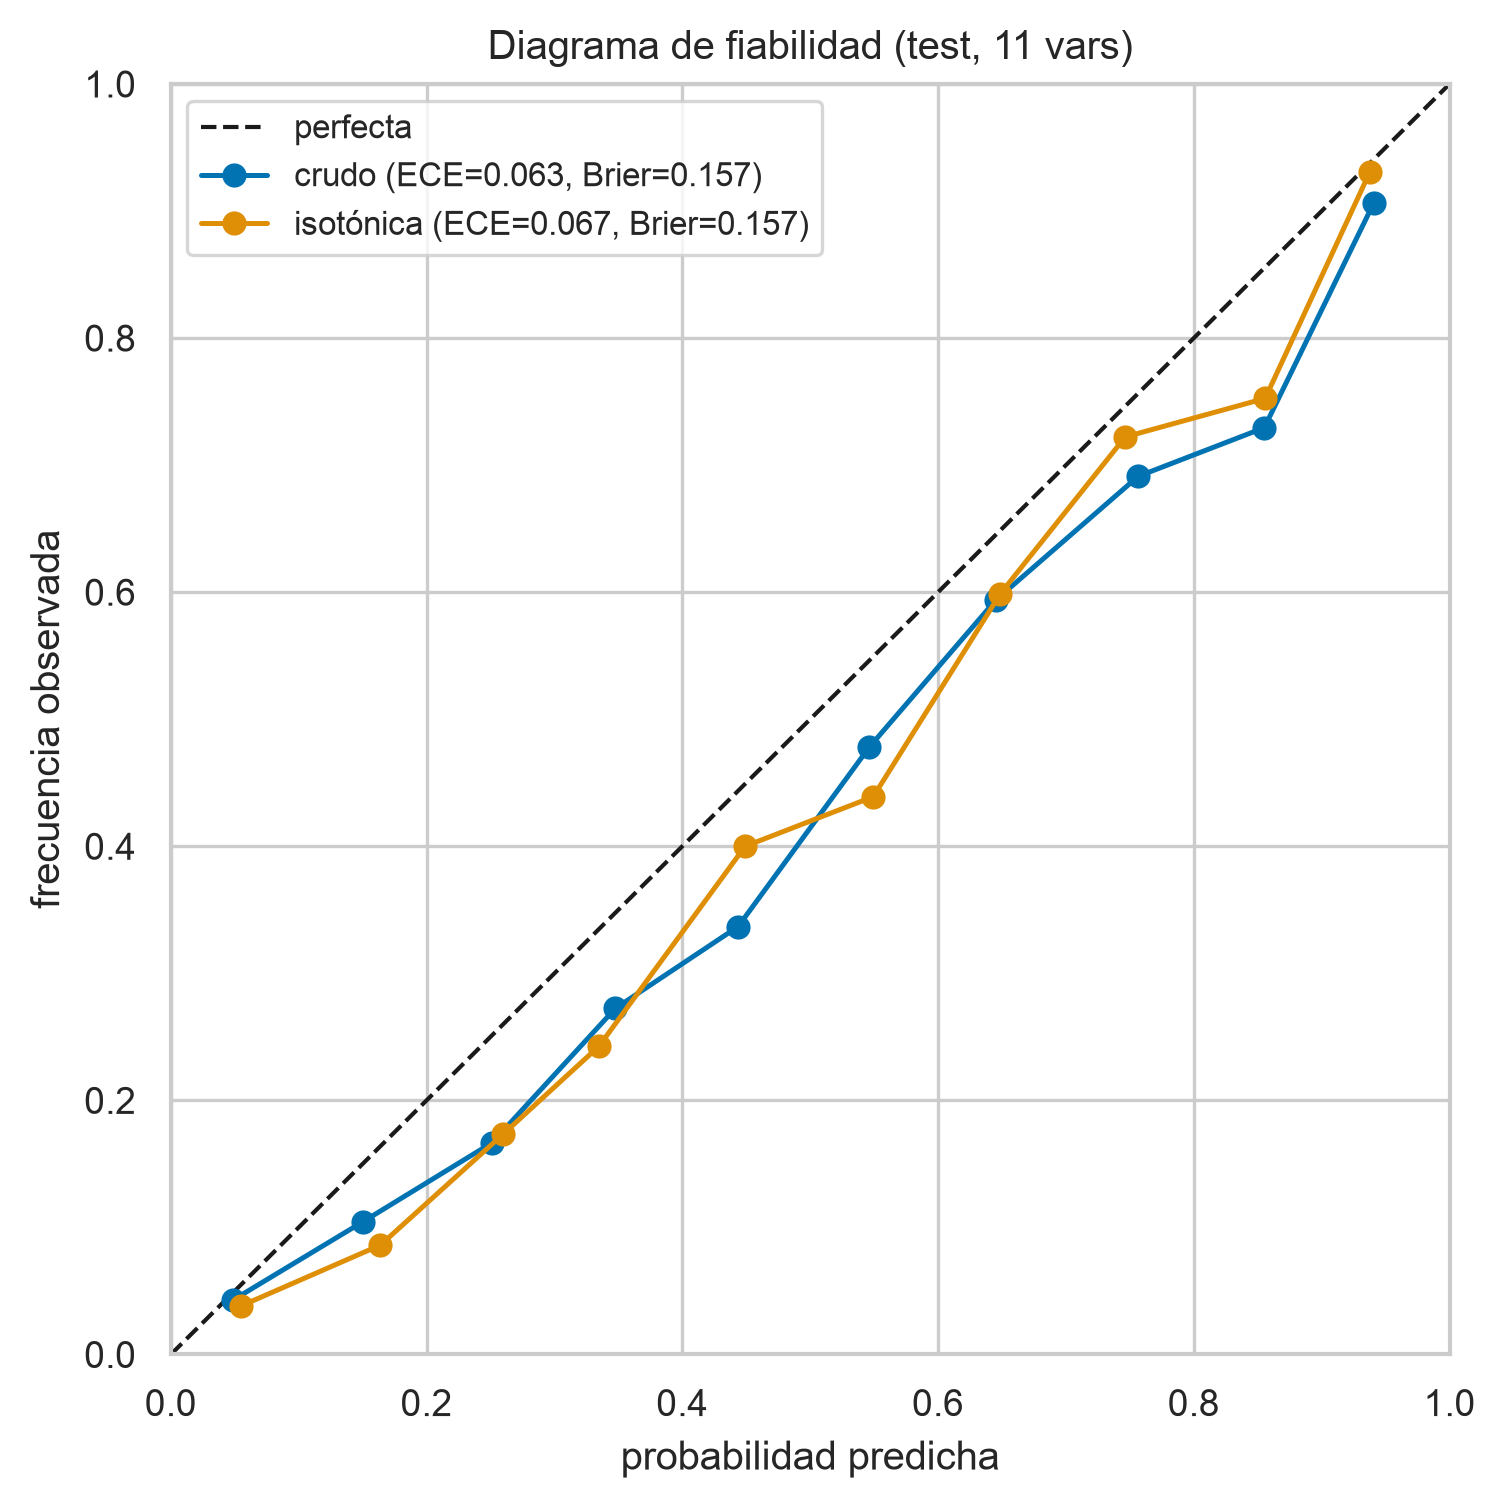
\includegraphics[width=\textwidth]{eval_calibracion}
\caption{Diagrama de fiabilidad.}
\label{fig:calib}
\end{subfigure}
\caption{Evaluación desagregada y calibración de XGBoost sobre el test oficial.}
\end{figure}

\section{Comparación con el estado del arte}

Situamos por fin el detector frente a la literatura sobre RAGTruth, que se mide en F1 a
nivel de respuesta y en accuracy, no en AUC. El Cuadro~\ref{tab:lit} y la
Figura~\ref{fig:lit} recogen la comparación por tarea. Nuestras cifras son las del punto
de operación por tarea sobre el test oficial.

\begin{table}[H]
\centering
\small
\begin{tabular}{lcccc}
\toprule
Método & QA & Data2txt & Summary & Global \\
\midrule
GPT-4-turbo (juez) & 45,6 & 78,3 & 47,6 & 63,4 \\
Luna (encoder ligero) & 51,3 & 75,9 & 52,5 & 65,4 \\
LettuceDetect-large (396M) & 70,2 & 88,5 & 59,7 & 79,2 \\
Fine-tuned Llama-2-13B & 68,2 & 88,1 & 59,1 & 78,7 \\
RAG-HAT (mejor) & 74,8 & 91,6 & 67,6 & \textbf{83,9} \\
\midrule
\textbf{Este trabajo (clásico)} & 49,2 & 82,1 & 45,3 & 65,6 / 68,4 \\
\bottomrule
\end{tabular}
\caption{F1 a nivel de respuesta (\%) sobre RAGTruth, recopilado por Kovács et al.
\cite{kovacs2025lettucedetect}, con RAG-HAT \cite{song2024raghat} como cota alta.
Nuestra columna global da el F1 macro por tarea (65,6) y el F1 pooled con umbral de
Youden (68,4). El patrón universal se repite: Data2txt fácil, QA y Summary difíciles.}
\label{tab:lit}
\end{table}

\begin{figure}[H]
\centering
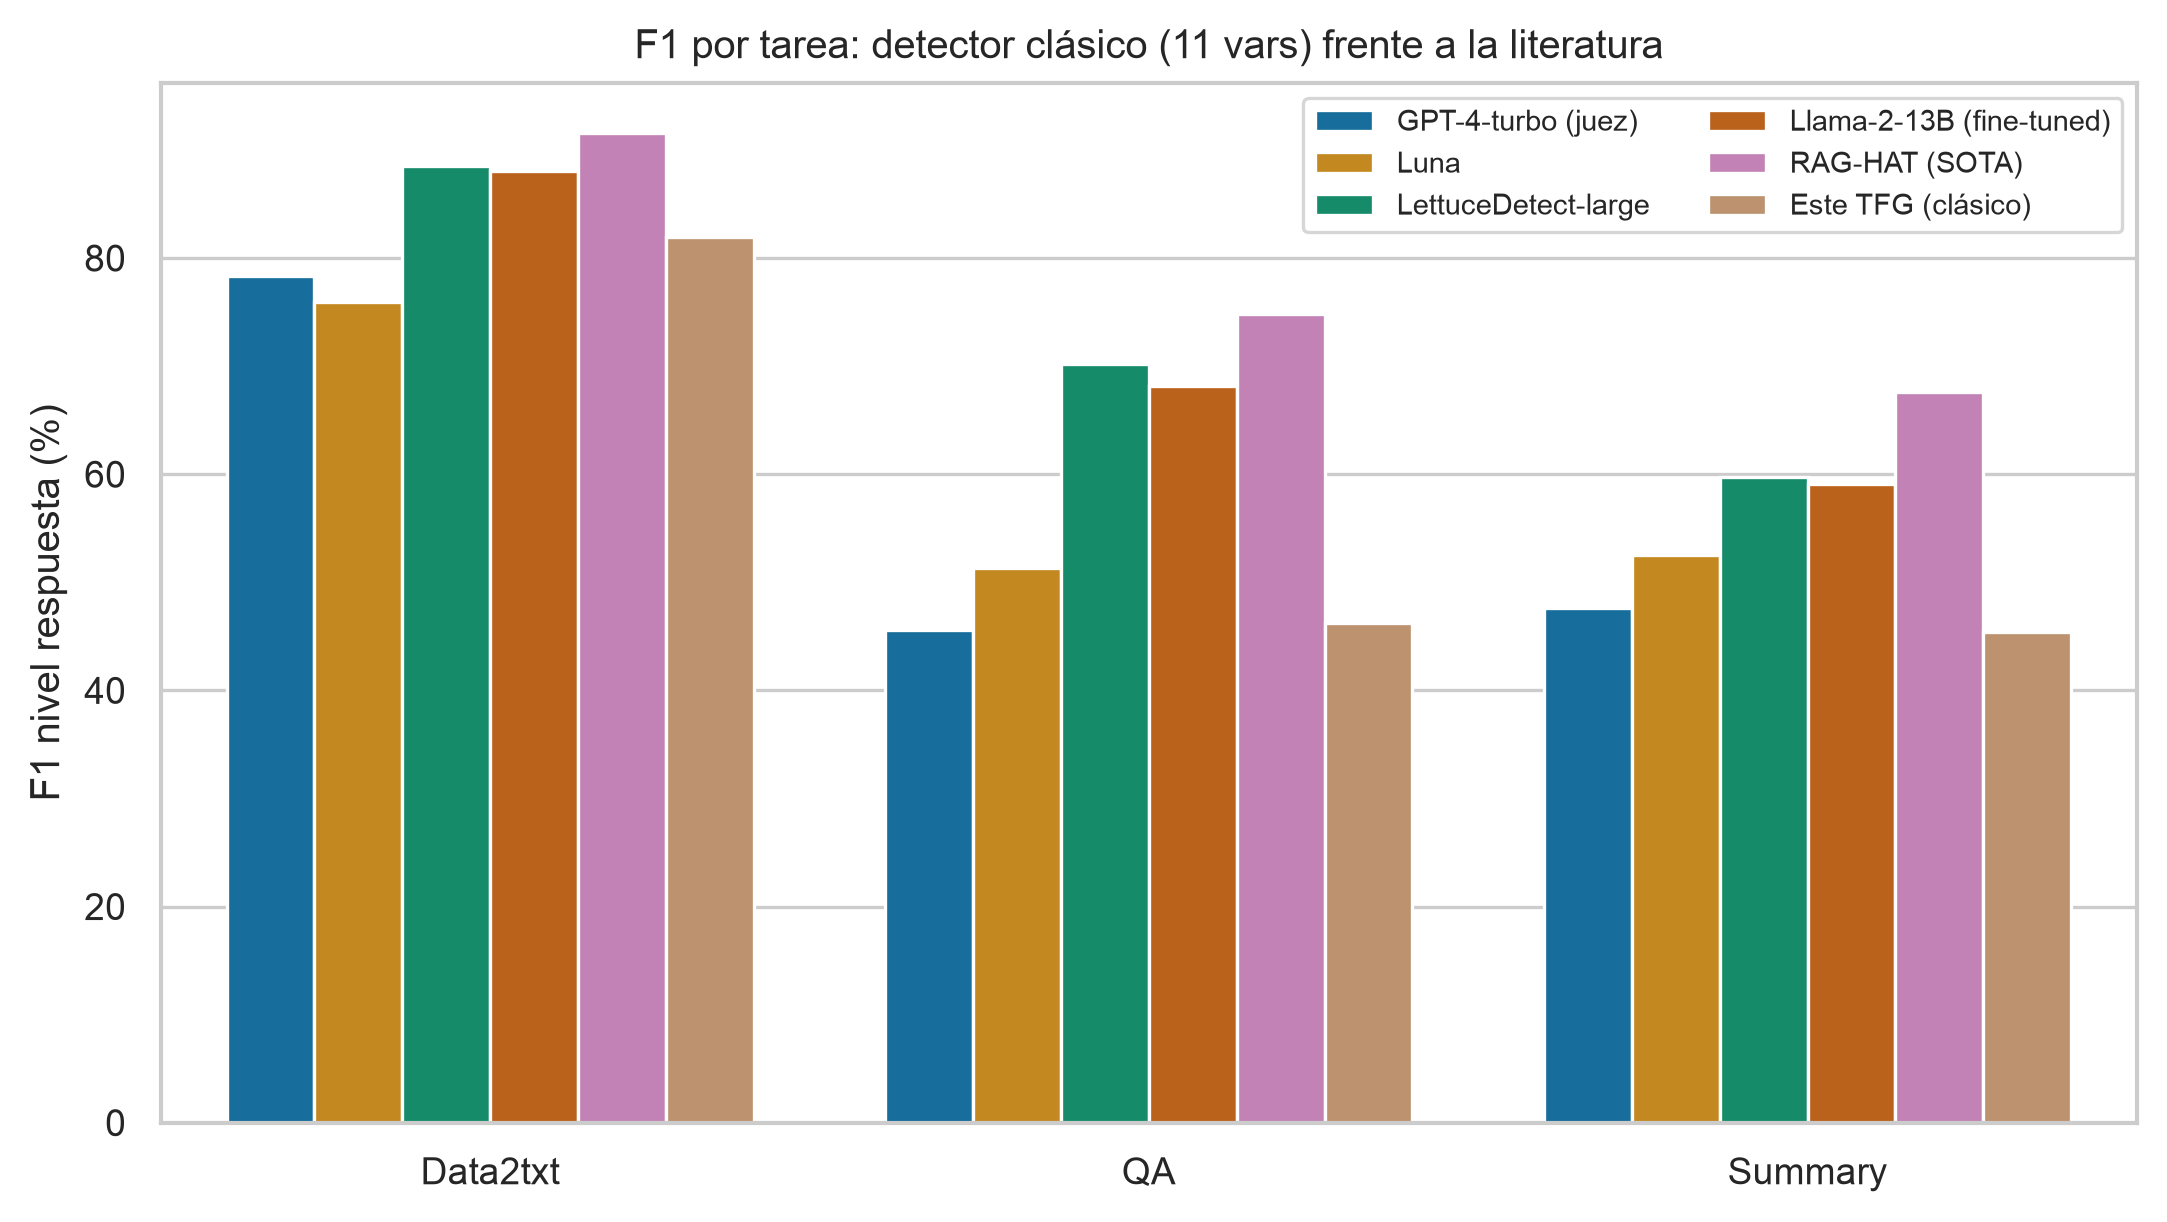
\includegraphics[width=\textwidth]{lit_comparacion_f1}
\caption{F1 por tarea, nuestro detector clásico frente a la literatura. La brecha se
concentra en Summary, la tarea que nadie resuelve con solvencia.}
\label{fig:lit}
\end{figure}

La lectura honesta es doble. En F1 global superamos al juez GPT-4-turbo (63,4) y a Luna
(65,4), y quedamos unos diez puntos por debajo de los modelos ajustados, LettuceDetect
(79,2), Llama-2-13B (78,7) y RAG-HAT (83,9). En accuracy sobre el subset RAGTruth, la
referencia es Lynx \cite{ravi2024lynx}, con Lynx-8B en 80,0 y GPT-4o en 84,3, mientras
nuestra accuracy ronda 0,74–0,78. El patrón por tarea es el mismo para todos: Data2txt
alrededor del 88--92\,\%, QA y Summary mucho más bajos. Chocamos contra el mismo muro
que modelos de miles de millones de parámetros, solo un poco antes. Un detalle refuerza
el valor del resultado: trabajos que analizan RAGTruth por activaciones sostienen que la
etiqueta apenas se correlaciona con diferencias de texto de superficie, de modo que
alcanzar 0,82--0,84 de AUC con características léxicas no es trivial.

\section{Conclusiones}

Recogemos las conclusiones objetivo por objetivo, como cierre del caso de estudio.

\paragraph{Hipótesis falsable.} Se cumple. Los cinco clasificadores clásicos superan el
AUC-ROC de 0,80 sobre el test oficial de RAGTruth con evaluación honesta, y el mejor
alcanza 0,836. Un clasificador clásico sobre características léxicas separa alucinación
de texto fiel con solvencia.

\paragraph{Falsos negativos y desbalance.} El déficit de recall no se debía a las
características ni al balance de clases, sino al punto de decisión bajo un desbalance
heterogéneo y con desplazamiento de prior. Un umbral por tarea recupera el 44\,\% de los
falsos negativos y hace competitivo el F1 de Summary. La corrección de prior de Saerens,
el remuestreo y el aprendizaje sensible al coste se descartaron con evidencia por no
mover la frontera.

\paragraph{El techo de Summary.} Está caracterizado, no supuesto. Cuatro familias de
características fracasan en Summary por la misma razón: resumir es recombinar, y el texto
fiel comparte la firma léxica con el alucinado. Es la frontera entre la minería clásica
de superficie y la semántica profunda, y el estado del arte, con modelos mucho mayores,
tropieza con el mismo muro.

\paragraph{Posicionamiento.} El detector rinde por encima del juez GPT-4-turbo y de Luna,
y a unos diez puntos de los detectores ajustados, a coste cero, en CPU, de forma
interpretable y determinista. Reproduce a bajo coste lo que hoy hace un evaluador basado
en modelos de lenguaje, y acota con precisión hasta dónde llega lo léxico.

\bibliographystyle{plain}
\bibliography{referencias}

\end{document}
